%% Copyright Notice: The United States Government retains, a nonexclusive, paid-up, irrevocable, worldwide license to publish or reproduce the published form of this work, or allow others to do so, for United States government purposes. This material is declared a work of the U.S. Government and is not subject to copyright protection in the United States. Approved for public release; distribution is unlimited.
%%
%% Contact lead author, Alex Kaszynski if you have any questions regarding this paper at the email below.

\documentclass[colorlinks,upint,subscriptcorrection,varvw,hyphenate,balance,govt]{asmeconf}

\usepackage{float}
\usepackage{siunitx}
\DeclareSIUnit{\inch}{in}
\DeclareSIUnit{\mil}{mil}
\DeclareSIUnit{\foot}{ft}

\hypersetup{%
	pdfauthor={Alex Kaszynski, Lucas Smith, Justin Warner, Jeffrey M. Brown},
	pdftitle={Experimental Investigation of As-manufactured Modeling for Integrally Bladed Rotor Frequencies and Mode Shapes},
	pdfkeywords={mistuning, integrally bladed rotors, mode shapes, manufacturing deviations, vibration testing, finite element modeling, mesh morphing, modal analysis, traveling wave excitation, structured light scanning, optical metrology, experimental validation, turbomachinery},
	pdfsubject={Experimental Investigation of As-manufactured Modeling for Integrally Bladed Rotor Frequencies and Mode Shapes},
}

\allowdisplaybreaks

\begin{document}

\ConfName{Proceedings of the ASME 2026\linebreak Turbomachinery Technical Congress and Exposition}
\ConfAcronym{TURBO2026}
\ConfDate{June 15--19, 2026}
\ConfCity{Milan, Italy}
\PaperNo{TURBO2026-179212}

\title{Experimental Investigation of As-manufactured Modeling for Integrally Bladed Rotor Frequencies and Mode Shapes}

\SetAuthors{%
    Alex Kaszynski\affil{2}\CorrespondingAuthor{alex.kaszynski@advanced-engineering-analysis.com},
    Lucas Smith\affil{1},
    Justin Warner\affil{1},
    Jeffrey M. Brown\affil{1},
}

\SetAffiliation{1}{Air Force Research Laboratory, Wright-Patterson Air Force Base, OH 45433}
\SetAffiliation{2}{Advanced Engineering Analysis LLC, Lafayette, CO 80026}

\maketitle

\begin{abstract}

    This work experimentally measures an academic rotor's mistuned system and blade-alone vibration behavior while validating an as-manufactured finite element modeling process. The model is created using blade geometry deviations captured with a structured light measurement system and a target-surface mesh morphing process. Geometry measurement uncertainty is established through repeated scans, and an uncertainty metric is used to ensure accuracy. Experimental vibration data for the academic rotor are acquired using a traveling-wave excitation system and a scanning laser vibrometer. A dense measurement grid provides a detailed characterization of blade mode shapes up to 10~kHz. Isolated blade-alone vibration data is collected to validate the mistuned system identification of the traveling wave data and for comparison with the as-manufactured model. The results show excellent correlation between the analytical model predictions and experimentally obtained measurements for modes in the wide frequency range, while also discovering significant blade mode shape variations at closely spaced mode families. The models' validity in this sensitive nonlinear region gives additional confidence in their use for mistuning analysis and experimental planning in turbomachinery applications.

\end{abstract}

\begin{nomenclature}[5.5em]

    \entry{EO}{Engine Order}
    \entry{FMM}{Fundamental Mistuning Model}
    \entry{FRAC}{Frequency Response Assurance Criteria}
    \entry{FRF}{Frequency Response Function}
    \entry{GMM}{Geometrically Mistuned Model}
    \entry{IBR}{Integrally Bladed Rotor}
    \entry{ICP}{Iterative Closest Point}
    \entry{MAC}{Modal Assurance Criterion, see Eq.~\ref{eq:mac} }
    \entry{OMA}{Operational Modal Analysis}
    \entry{TWE}{Traveling Wave Excitation}
    \entry{pLSRA}{Polyreference Least Squares Rational Approximation}
    \entry{$\mathrm{MSE}$}{Mean squared error}
    \entry{$\phi_{ik}$}{Mode shape at measurement point $i$ for mode $k$ }
    \entry{$\omega_{n,k}$}{Natural frequency of mode $k$ [Hz]}
    \entry{$\zeta_k$}{Damping ratio of mode $k$ }
    \entry{$\Delta_\omega$}{Normalized sector mistuning deviation }
    \entry{$H_i(\omega)$}{Complex frequency response function (FRF) at measurement point $i$ }
    \entry{$\mathbf{H}(\omega)$}{FRF measurement matrix, see Eq.~\ref{eq:frf_matrix} }
    \entry{$N_i(s)$}{Numerator polynomial of FRF at measurement point $i$ }
    \entry{$D(s)$}{Denominator polynomial of FRF }
    \entry{$s_k$}{Poles of the system [rad/s]}
    \entry{$\bar{x}, \bar{y}$}{Mean values of $x$ and $y$ for FRAC calculation }
    \entry{$\mathbf{Y}$}{Measured FRF data matrix }
    \entry{$\mathbf{P}$}{Frequency-dependent modal matrix }
    \entry{$\mathbf{O}$}{Modal constants and residuals matrix }
    \entry{$\overline{\mathrm{MAC}}_{i=j}$}{Mean diagonal blade MAC score}
    \entry{$\overline{\mathrm{MAC}}_{i<j}$}{Upper triangle mean of MAC between blade mode shapes, see Eq.~\ref{eq:mac_upper} }
    \entry{$r_{\Delta_{\omega}{\text{FMM},\text{GMM}}}$}{Correlation between the GMM and FMM sector mistuning deviations}

\end{nomenclature}

\section{Introduction}

Integrally bladed rotors (IBRs) have been widely adopted in military and commercial gas turbine engines due to their aerodynamic efficiency and structural simplicity. However, the absence of airfoil dovetail and fir-tree interfaces reduces structural damping and leads to increased vibratory stress. Mistuning from blade-to-blade variations in geometry and material properties further adds to response amplification. The ability to predict and experimentally validate mistuned vibratory response has been an ongoing research area, and the present work contributes new insights into as-manufactured modeling of IBRs and their ability to predict mistuned behavior across a wide frequency range, including closely spaced mode families that experience mode shape distortion.

Prior efforts to model mistuned response developed finite element–based reduced-order models (ROMs) that assumed nominal mode approximations and represented blade-to-blade mistuning as variations in blade-alone or mistuned system modal stiffness\cite{Castanier1997, Yang1999, Feiner2002, Lim2007}. Tools like these made a significant impact on design practices, but had two limitations. First, these tools did not provide a modeling approach to determine the modal stiffness variations. This capability is needed to predict the behavior of as-manufactured parts. Second, the models did not account for blade-specific mode shape variations. These mode shape variations can arise from either small geometric deviations inherent to manufacturing \cite{Beck2013}, or large geometric deviations from damage or blend repairs \cite{Madden2012}.

Researchers developed mistuned system identification algorithms and testing procedures to address the first limitation of these ROMs \cite{Feiner2004, Judge2009, Waldherr2020, Kelly2022}. The methods reformulate the ROMs to solve for blade-specific modal stiffnesses when given experimentally measured system modes and responses. The identified system can then be used in follow-on analysis across a wider range of operating conditions and support tailored management of manufactured parts and fielded components.

Others have focused on processes to create as-manufactured finite element models (FEMs) that predict geometric variation effects on blade modal stiffness and mode shapes. This solves both of the challenges of nominal mode mistuning ROMs and can leverage measurement data taken during manufacturing. As-manufactured FEMs can be created using cross-sectional data from coordinate measurement machines (CMMs) \cite{Brown2003, Sinha2008, Bouras2024} or dense point clouds from structured light scanning systems \cite{Schoenenborn2009, Kaszynski2014, Maywald2017}. These as-manufactured FEMs can predict the variations in modal behavior across the range of operational thermal and structural loads. The geometry measurement data can further be used to determine variations in unsteady aerodynamic loading caused by geometry \cite{Clark2018}. Multiple efforts have developed geometrically mistuned system ROMs that expand the capabilities of as-manufactured modeling for small and large deviations \cite{Sinha2009, Beck2014, Baek2017, Bouras2024}. As with the nominal mode models, these geometric ROMs have developed into geometric mistuning system identification capabilities \cite{Bhartiya2014, Beck2023}.

Experimental validation of these as-manufactured models has been an ongoing area of research. Several efforts have used techniques that isolate a single blade, collect vibration data with a laser Doppler velocimeter (LDV), and excite with impact hammers. For blade isolation, Schonenborn et al.\ used damping material \cite{Schoenenborn2009}, while Maywald et al.\ and Popig et al.\ used magnetic masses attached to blade edges \cite{Maywald2017, Popig2015}. Zhou et al.\ used the same isolation approach, but used an improved blade-alone frequency identification process with an analytical correction technique \cite{Zhou2022}. Nakos et al.\ performed similar testing and further modified the correction capability \cite{Nakos2025}. Additional improvement to blade isolation was shown by Langheinrich et al.\ who performed their blade detuning testing within a vacuum chamber to significantly reduce mode coupling \cite{Langheinrich2024}. Kaszynski et al.\ used traveling wave testing and mistuned system identification to validate their models, rather than physical blade isolation \cite{Kaszynski2015}. These works all showed that as-manufactured FEM can accurately predict blade-to-blade frequency variations in certain frequency ranges. Each effort used a single LDV measurement point per blade to measure response and therefore did not investigate the as-manufactured model's ability to predict mode shapes and their variation.

Several researchers, however, have shown that airfoil mode shapes can vary, particularly for closely spaced modes \cite{Brown2019, Bae2019}. Gillaugh et al.\ further demonstrated the impact of these mode shape variations on strain gauge and non-intrusive stress measurement system (NSMS) data processing \cite{Gillaugh2018, Gillaugh2019}. These efforts used predicted blade mode shape variations as part of their method developments, but they did not experimentally demonstrate their accuracy.

The present work contributes new processes and validation of as-manufactured modeling of mistuned rotors with an emphasis on blade mode shape variations. An accurate as-manufactured FEM is created through mesh morphing structured light measurement data generated from an iterative process, enabling measurement error reduction. The results from this model are compared to experimental data generated by a traveling wave excitation (TWE) system and LDV measurements of 185 measurement points per airfoil of the 20-bladed academic test rotor. The dense pattern of blade vibration measurements is used to validate the as-manufactured model's ability to predict interblade mode shape variations with a focus on extreme variation of a closely spaced mode pair. Experimental data is collected for the mistuned rotor and isolated blades testing that applied mass detuning and blade damping. Mistuned system identification based on the fundamental mistuning model (FMM)\cite{Feiner2002} is used to extract blade mistuning parameters, and polyreference least square rational approximation (pLSRA) is used to identify isolated blade test frequencies when mode coupling is not fully eliminated. Results are reported for a wide range of mode families, up to 10 kHz, highlighting both the accuracy of the as-manufactured model and the complex mode shape distortions of closely spaced blade resonances.

\section{Experimental Setup}

\subsection{Test Article}
The subject rotor of this work is the Parametric Blade Study (PBS) Rotor 5. It was one of eight rotors developed in the 1980s for design and testing purposes. Each rotor varied one geometry parameter to monitor its effect on the stage's performance. This rotor is a close relative of the PBS Rotor 4, which has been the subject of recent mistuning research \cite{Gillaugh2018, Gillaugh2019}. PBS Rotor 5 shares the 20 blade count and is similarly manufactured from Ti-6Al-4V, which has a reflective surface that can be a challenge for optical scanning systems. While anti-reflective coatings such as titanium dioxide can be applied in such cases, this was not done in this work in order to obtain geometry measurements with a minimum of processing steps.

\subsection{Optical Geometry Measurement}

\begin{figure}
    \centering
    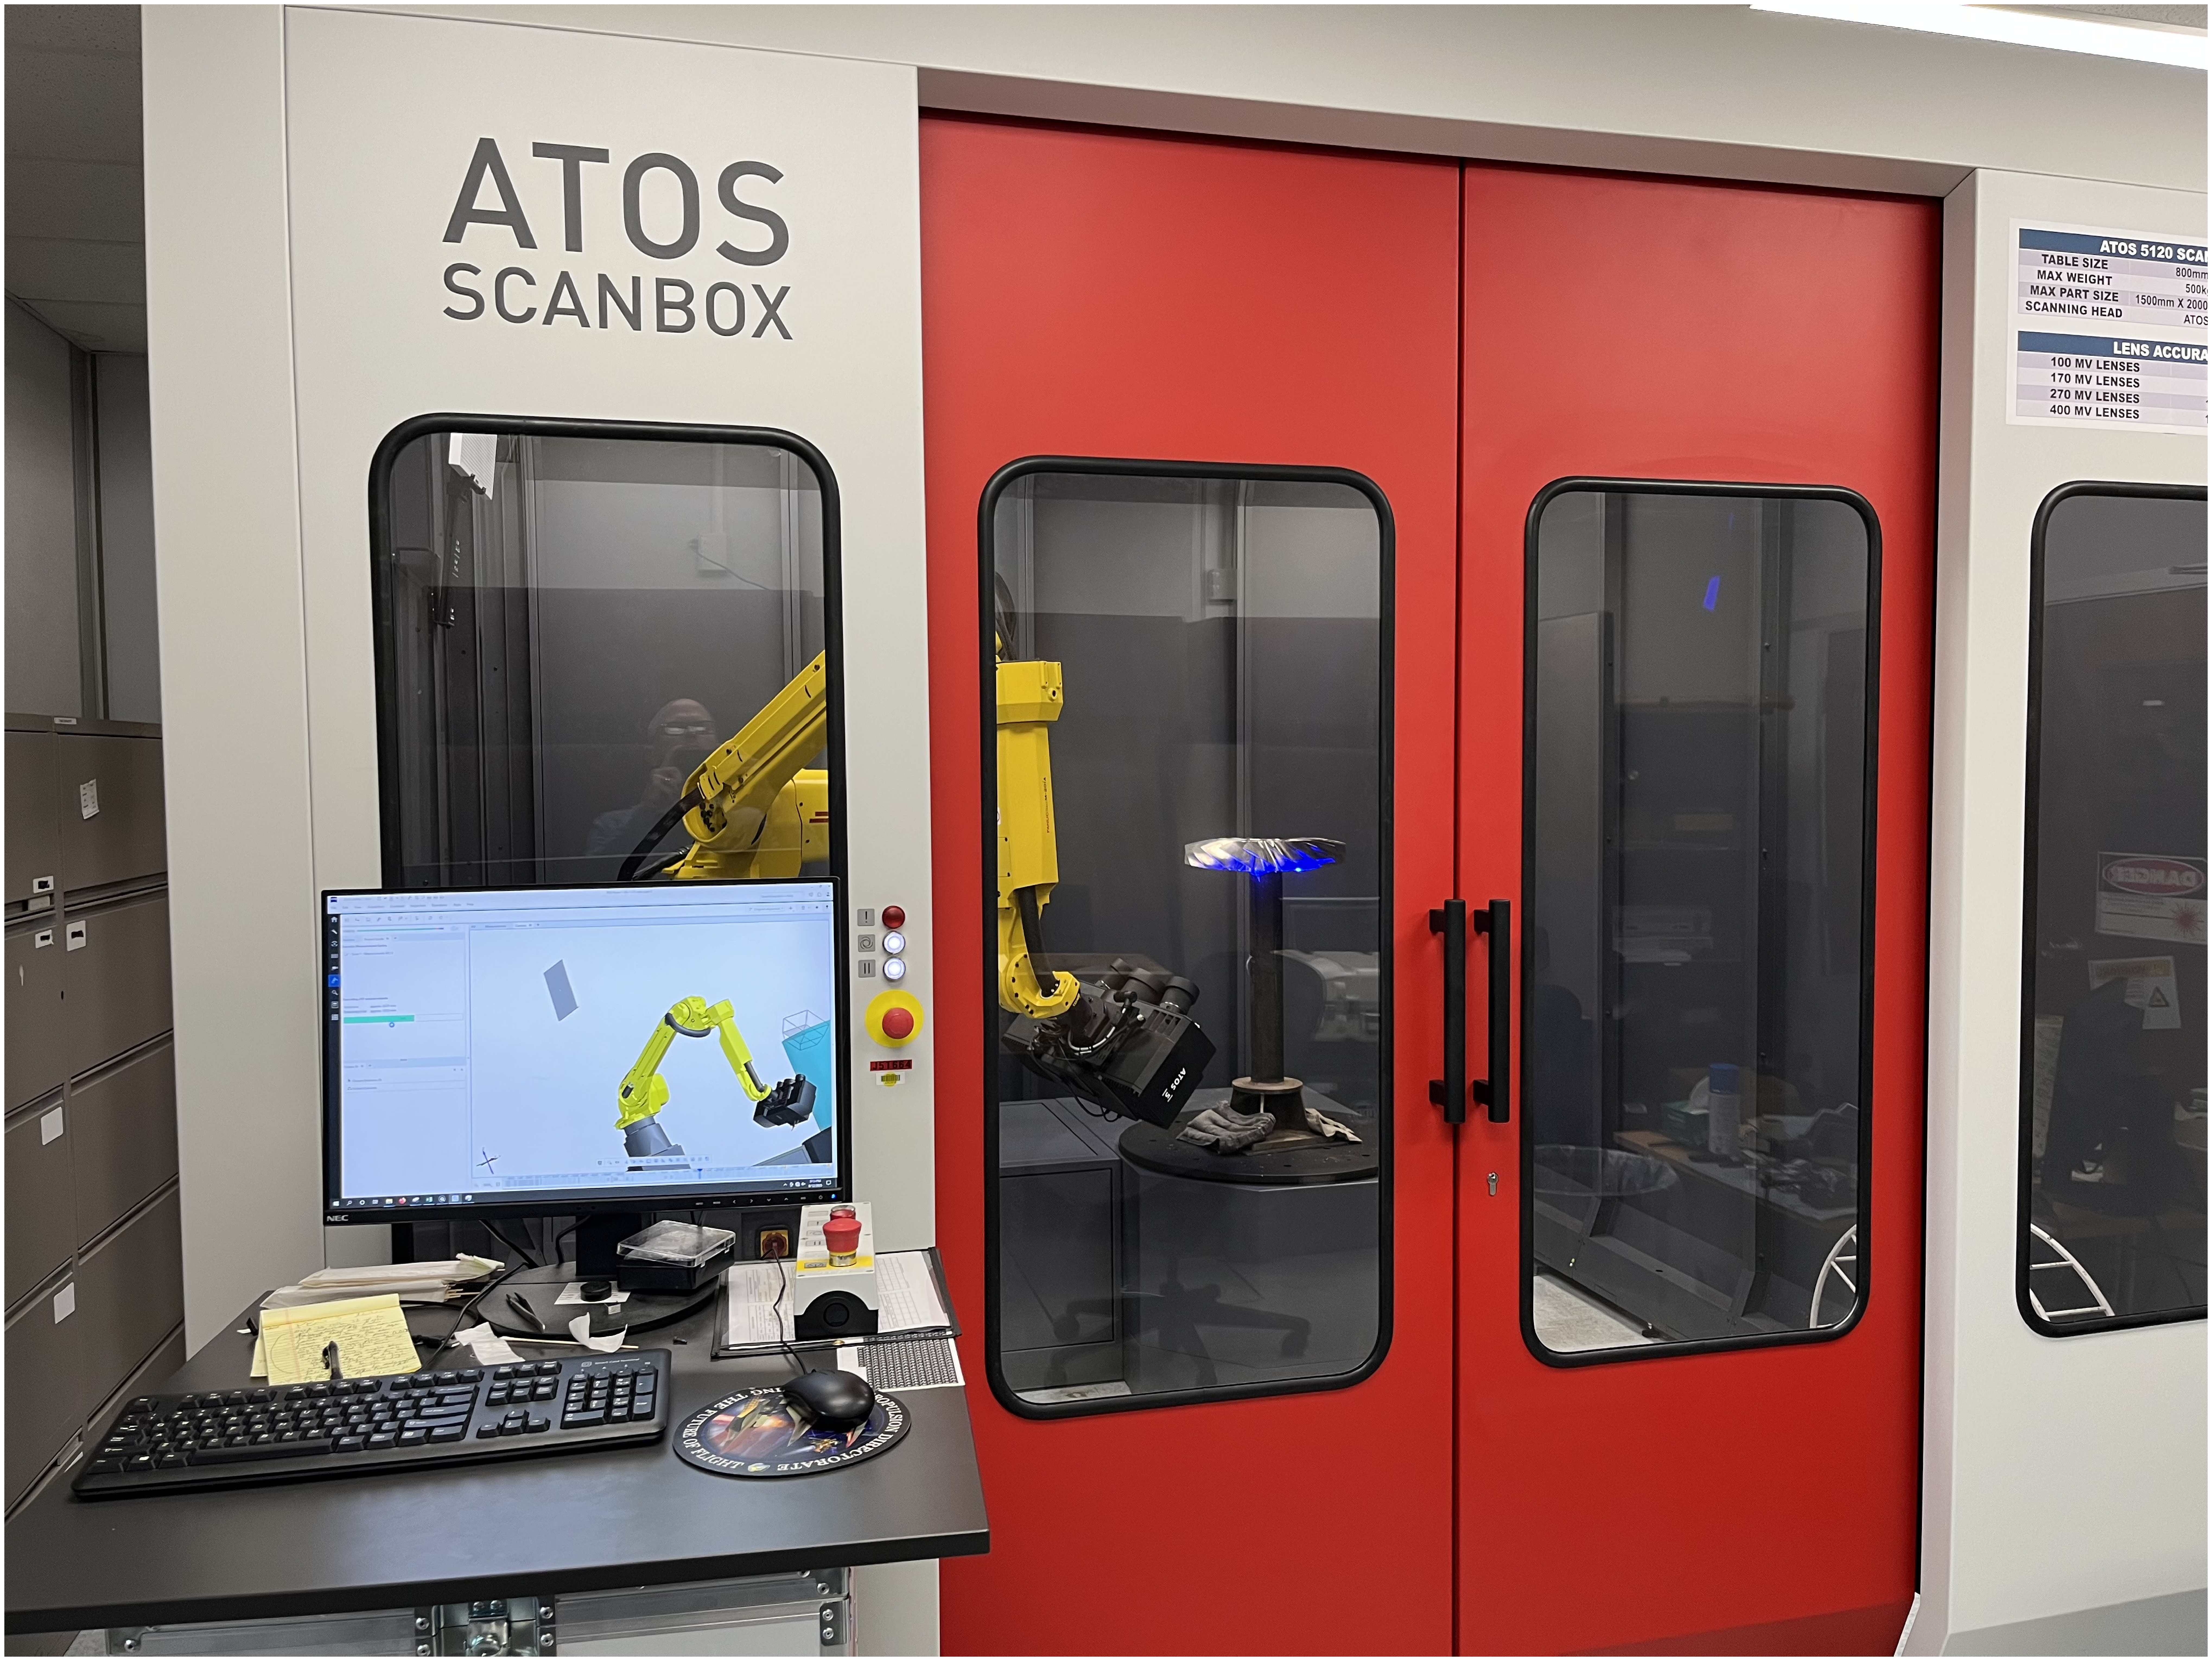
\includegraphics[width=\linewidth, alt = {ATOS Scanner Setup}]{figures/Figure1.eps}
    \caption{ATOS Scanbox 5120 measuring PBS rotor 5}
    \label{atos_scanner_setup}
\end{figure}

The test article was measured using a ZEISS ATOS 5 Airfoil structured light scanner within a ZEISS ScanBox 5120 for automation, as shown in Figure \ref{atos_scanner_setup}. The rotor geometry was collected using a \SI{270}{\milli\metre\cubed} lens scanning volume, with an expected accuracy of \SI{0.3937}{\mil} (\SI{10}{\micro\meter}) or better. The rotor was shaft-mounted approximately \SI{2}{\foot} (\SI{0.61}{\metre}) above the rotating measurement table to allow geometry capture below and above the part. At least 24 individual image captures were taken per rotor to ensure full rotor surface measurement.

The PBS rotor was scanned 6 times using an automated scanning procedure for consistency and aligned with MAGSAC \cite{barath2019magsac} and FEMORPH \cite{Kaszynski2014} to a nominal cyclically symmetric FEM using point feature histogram (PFH) global registration. Next, all 6 scans were locally registered to each other to minimize intra-surface distance using Anderson accelerated iterative closest point (ICP).

\begin{figure}[!b]
    \centering
    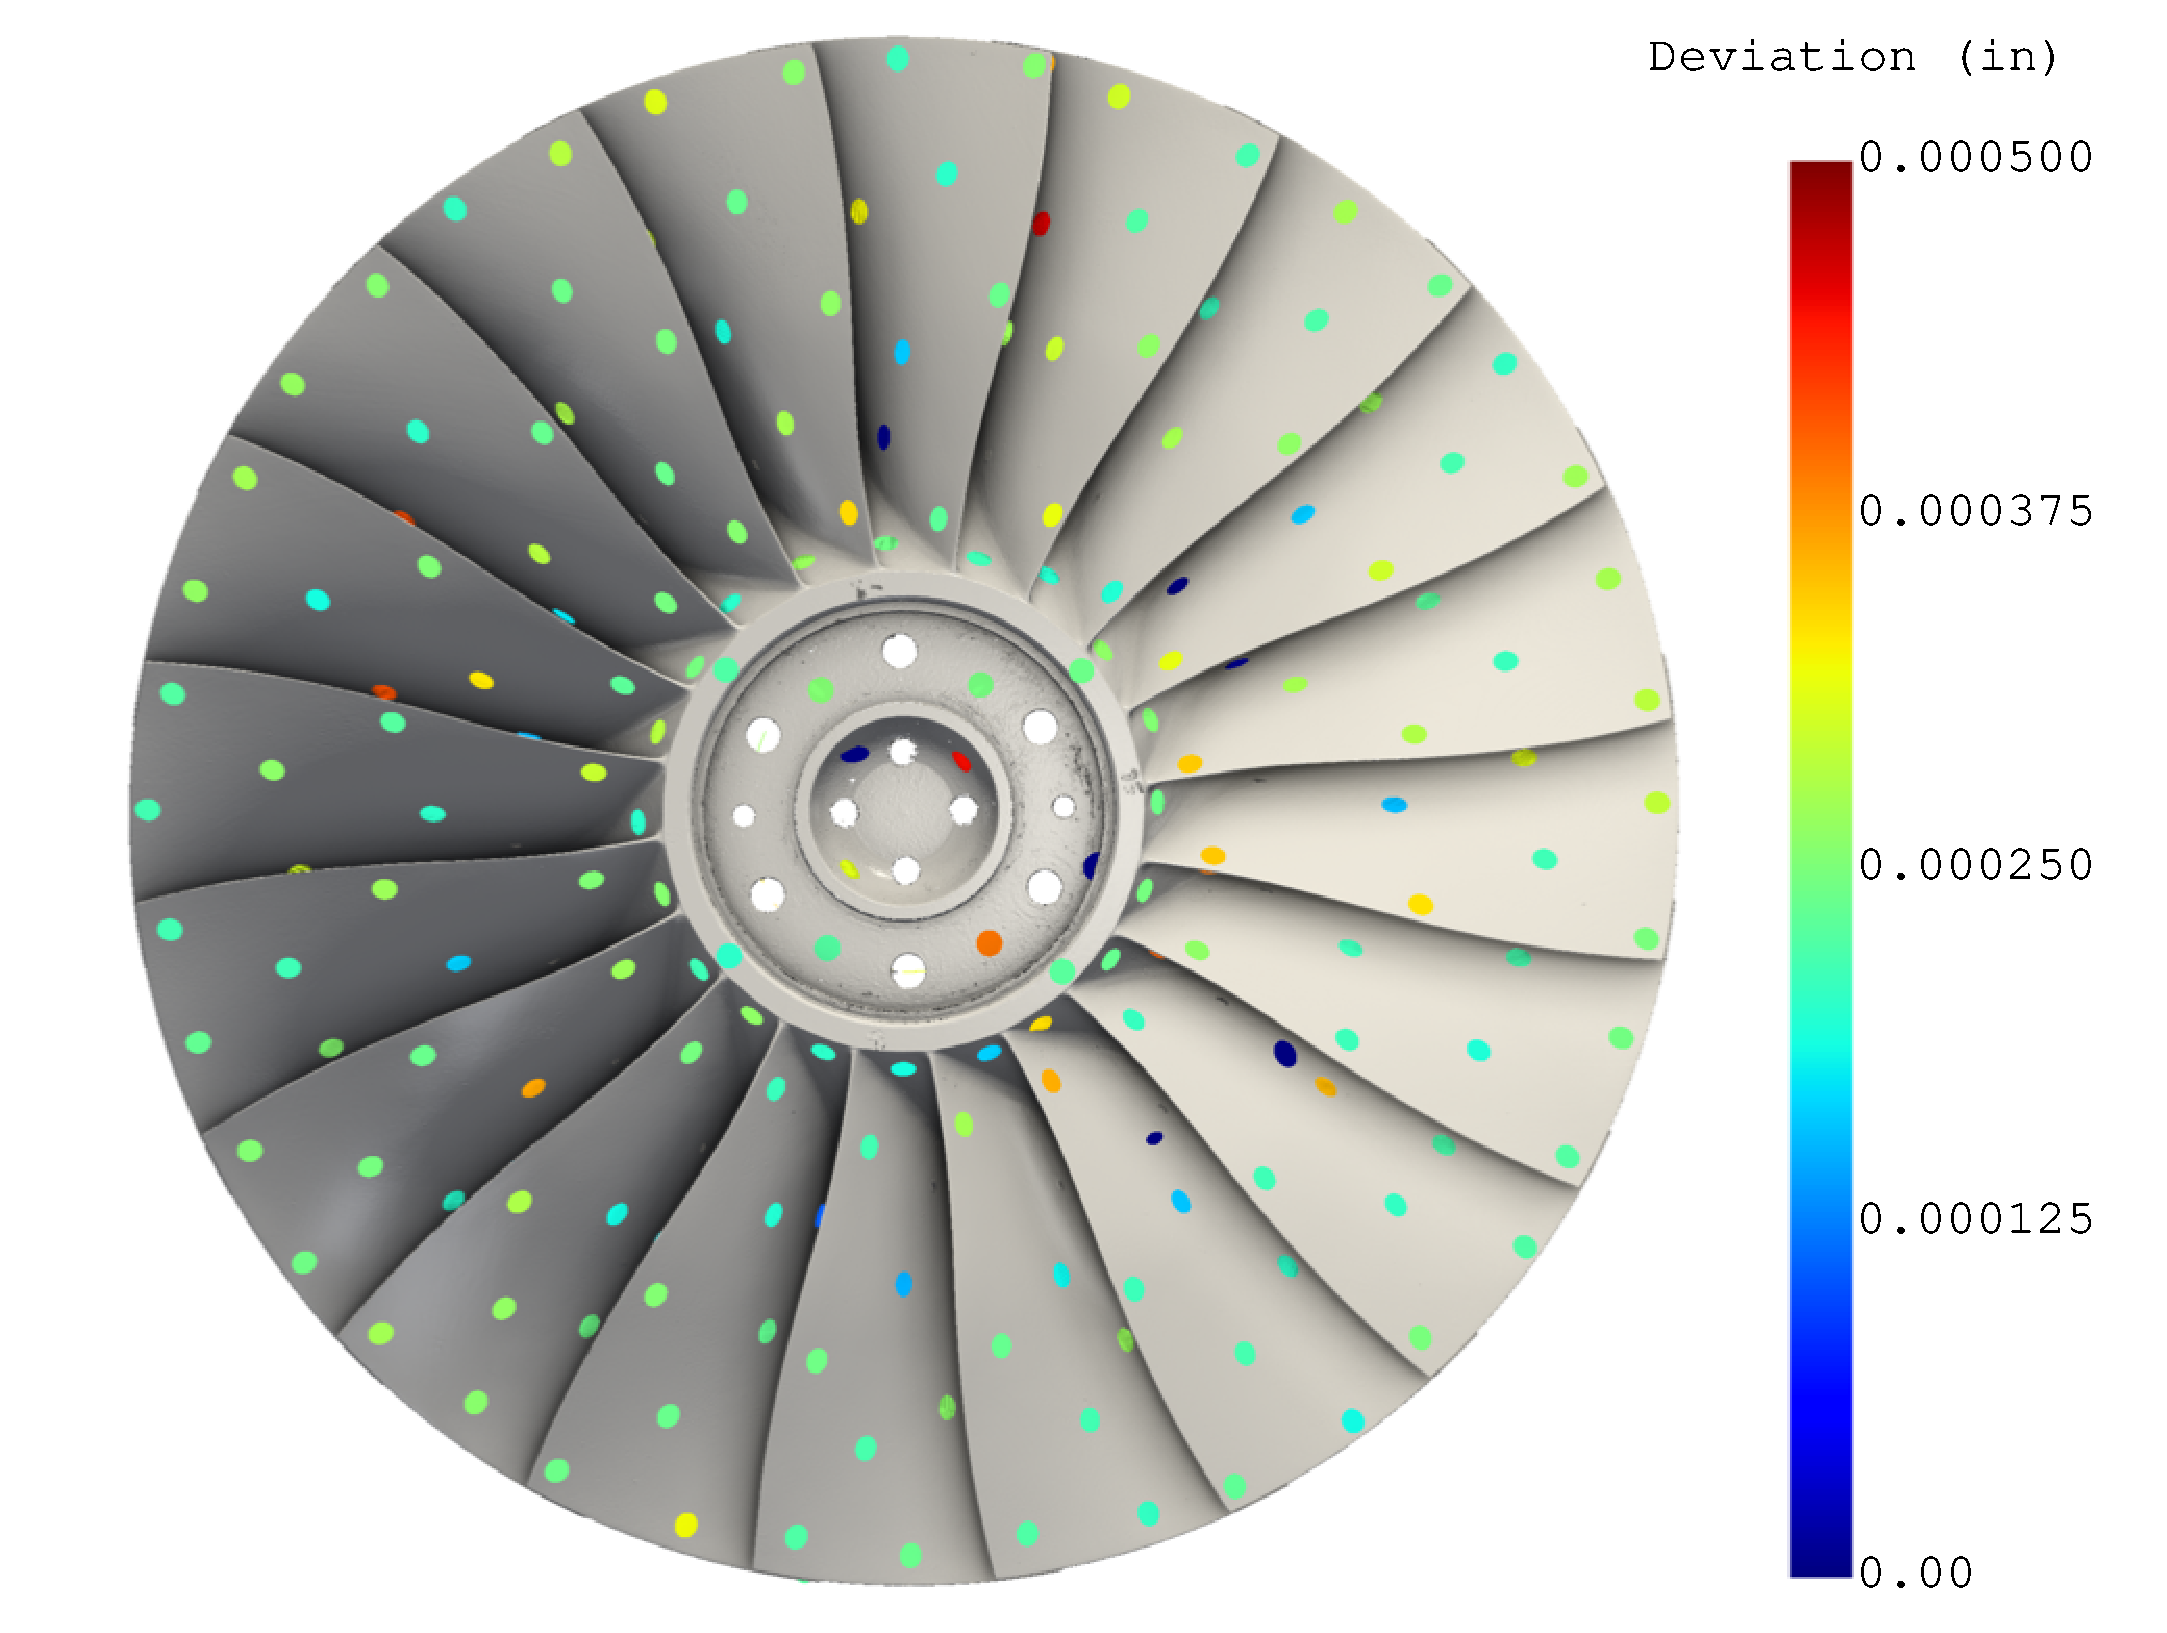
\includegraphics[width=\linewidth, alt = {Reference Point Deviation}]{figures/ref-point-deviation/Figure2.eps}
    \caption{Reference point deviation}
    \label{fig:reference_point_deviation}
\end{figure}

Scan accuracy was calculated by both comparing the reference point registration error from the ZEISS Inspect scanning software and the mean intra-scan surface distance between all six registered scans. On average, the reference point registration error was \SI{0.2556}{\mil} (\SI{6.492}{\micro\metre}) across all six scans, with scan 6 shown in Figure \ref{fig:reference_point_deviation}. The number of reference points was increased as the scanning progressed, and the reference point deviation varied from \SI{0.2876}{\mil} to \SI{0.2120}{\mil} (\SI{7.305}{\micro\metre} to \SI{5.385}{\micro\metre}), with the error falling as the number of reference points increased. The registration point error closely agreed with the mean intra-scan surface variation of \SI{0.3916}{\mil} (\SI{9.957}{\micro\metre}) between all six scans, demonstrating its effective use as a proxy for scan quality for quality control purposes. See Figure \ref{fig:scan_surface_deviation} for the surface-to-surface deviation between scans 5 and 6.

Each of the six scans was used to create an as-manufactured FEM. The deviation between scans 5 and 6 is within the expected measurement error range, and therefore, the sixth scan was used as the primary data set for which the finite element analysis (FEA) results are shown. The FEA results were not sensitive to the scan-to-scan variations, except for the mode shape variation of a closely spaced mode pair, which will be discussed further in an upcoming section. The as-manufactured model from scan 6 of the IBR, for conciseness and specificity, will be referred to for the remainder of the paper as a geometrically mistuned model (GMM).

\begin{figure}
    \centering
    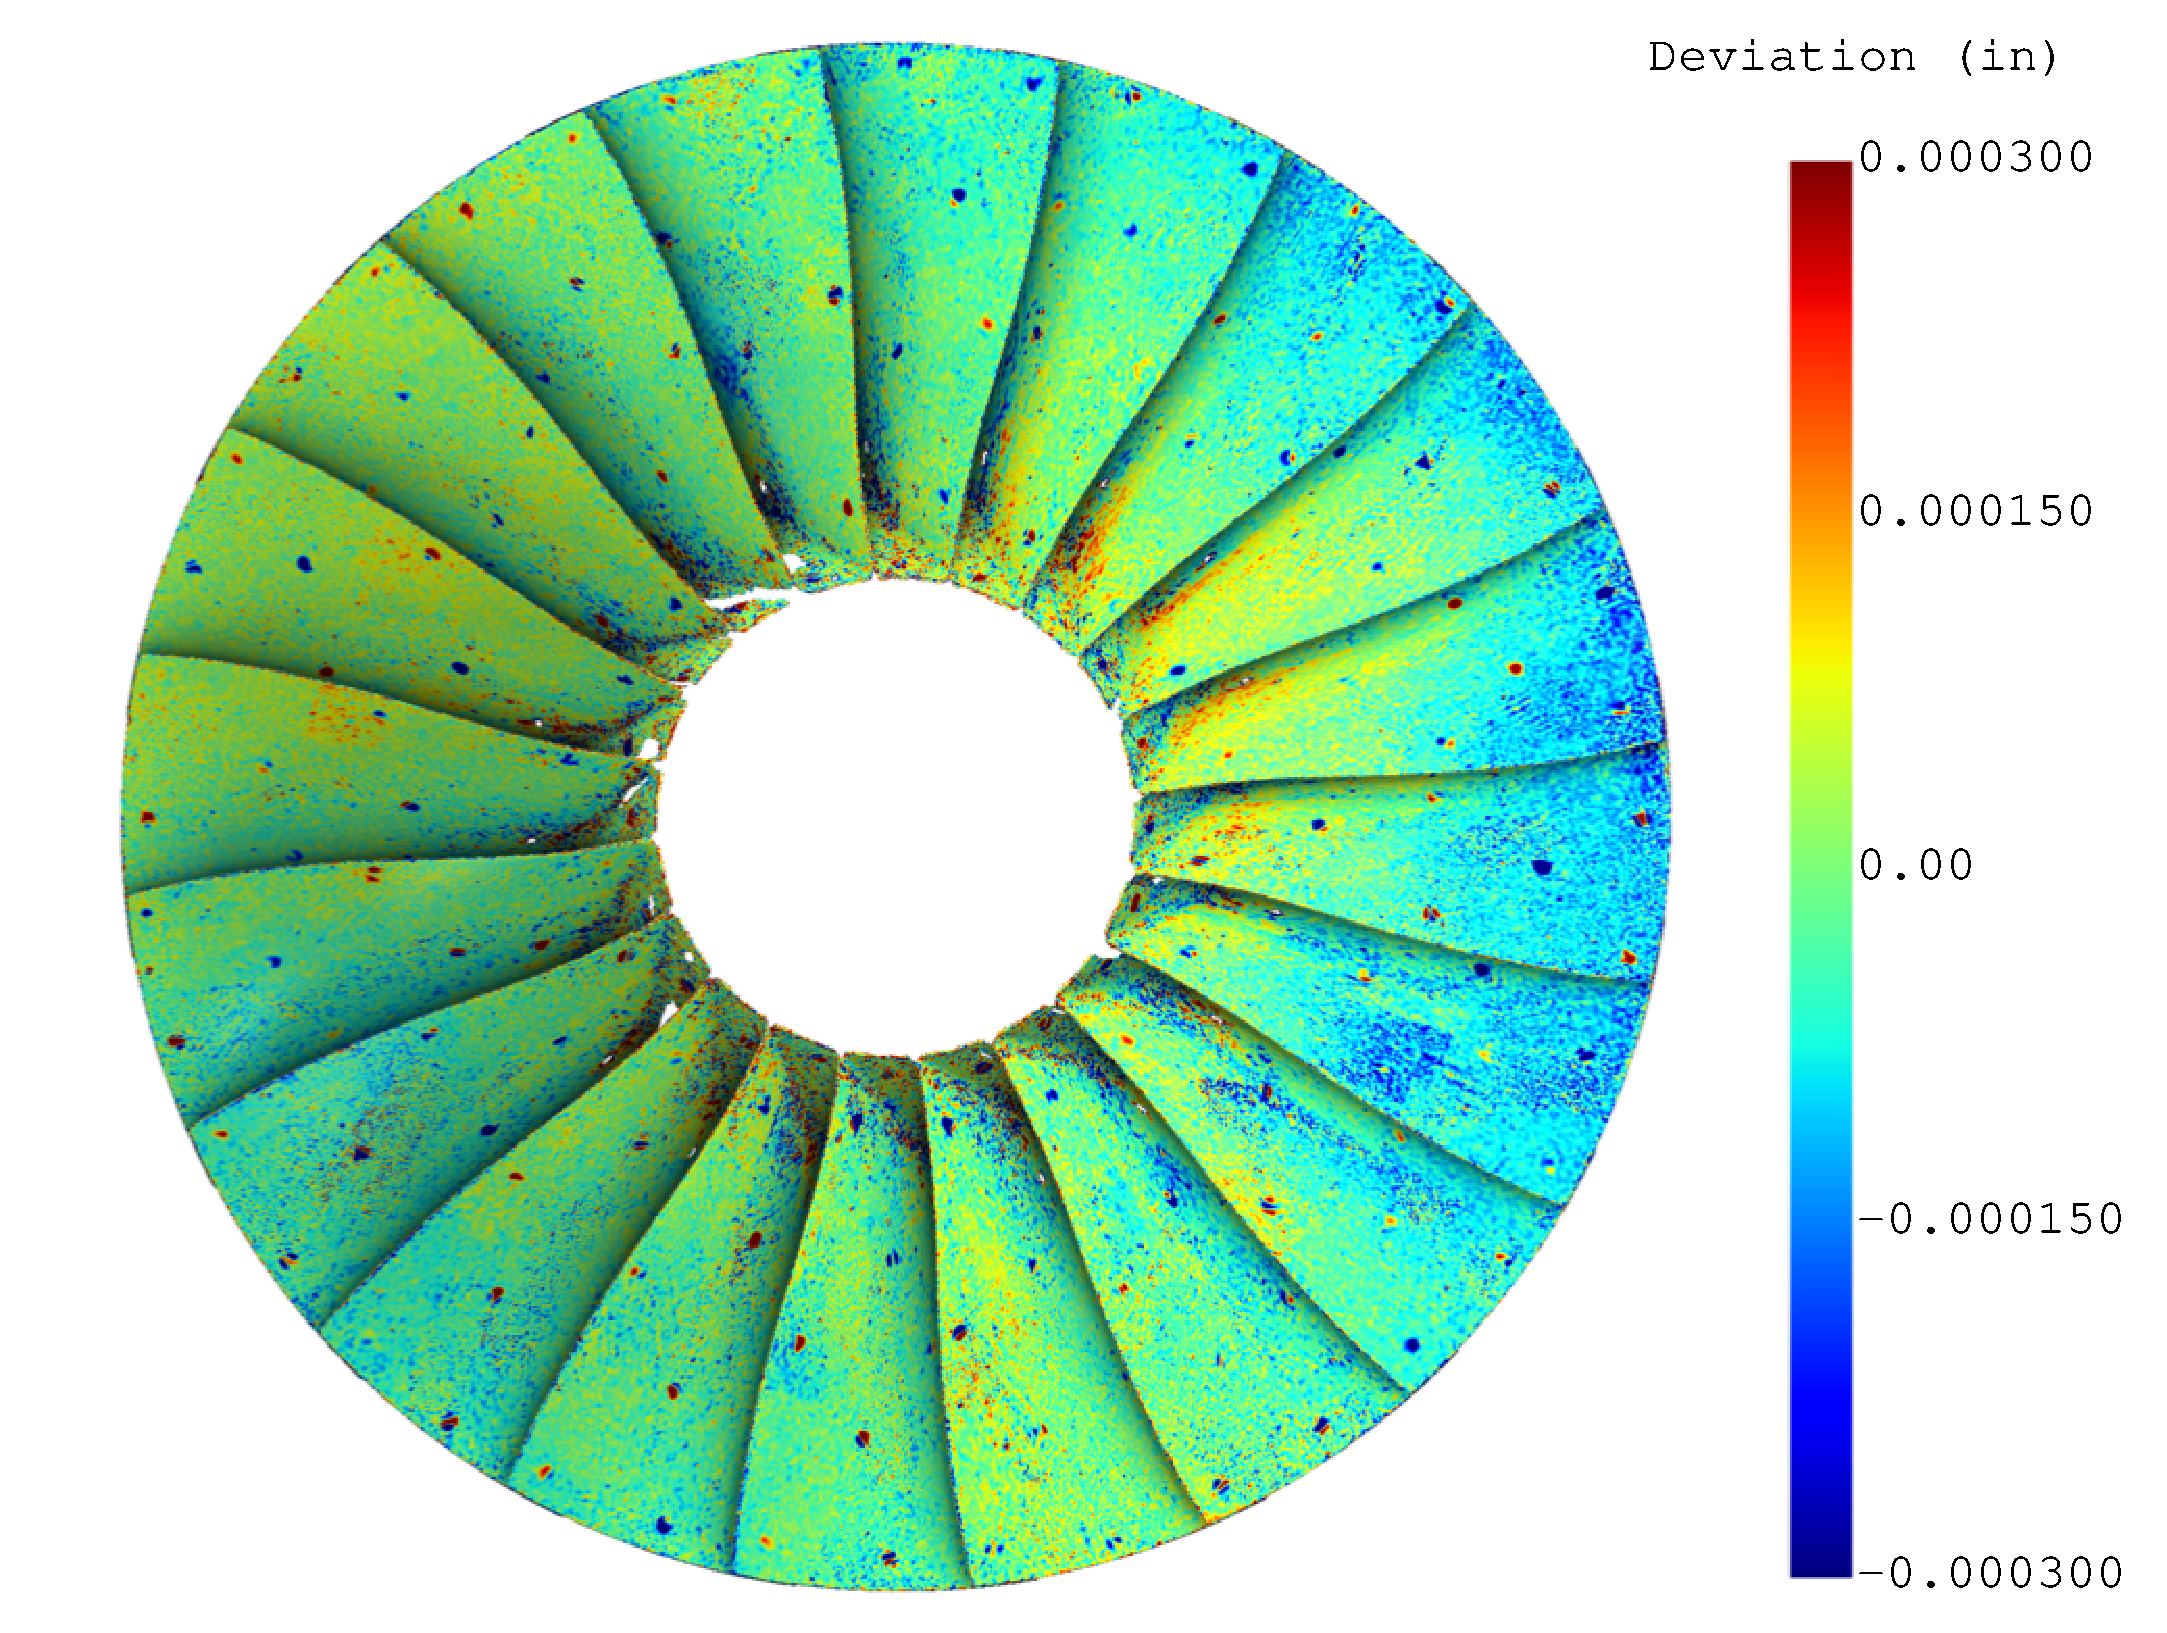
\includegraphics[width=\linewidth, alt = {Scan 5 and 6 Surface Variation}]{figures/scan-to-scan-variation/Figure3.eps}
    \caption{Scans 5 and 6 surface variation}
    \label{fig:scan_surface_deviation}
\end{figure}

\subsection{Traveling Wave Vibration Testing}

Validation of the analytical mode shapes and predicted frequency response requires both isolated blade and full rotor response operational modal analysis (OMA). The traveling wave experimental test setup was conducted to identify the mistuned mode families mode shapes, frequency ranges, and observed sector mistuning deviations calculated using FMM ID \cite{Feiner2004}. To perform TWE testing, high frequency speakers capable of up to 25 kHz excitation were placed at the tip of the leading edge of each of the 20 blades. The standard form of the TWE excitation applied circumferentially to an $N_b$-bladed rotor is

\begin{equation}\label{eq:tw_excitation}
    F_k(t) = F_0 \cos\Big(\omega t + \frac{2\pi m}{N_b} k \Big), \quad k = 0, \dots, N_b-1
\end{equation}

\noindent where \(F_0\) is the excitation amplitude, \(\omega = 2\pi f\) is the angular frequency [rad/s], \(m\) is the engine order (EO), \(N_b\) is the number of blades, and \(k\) the blade index. This signal was produced with National Instruments analog signal generators driving audio amplifiers via a chirp signal created by modulating the amplitude and phase for each blade according to Equation ~\eqref{eq:tw_excitation}.

\begin{figure}
    \centering
    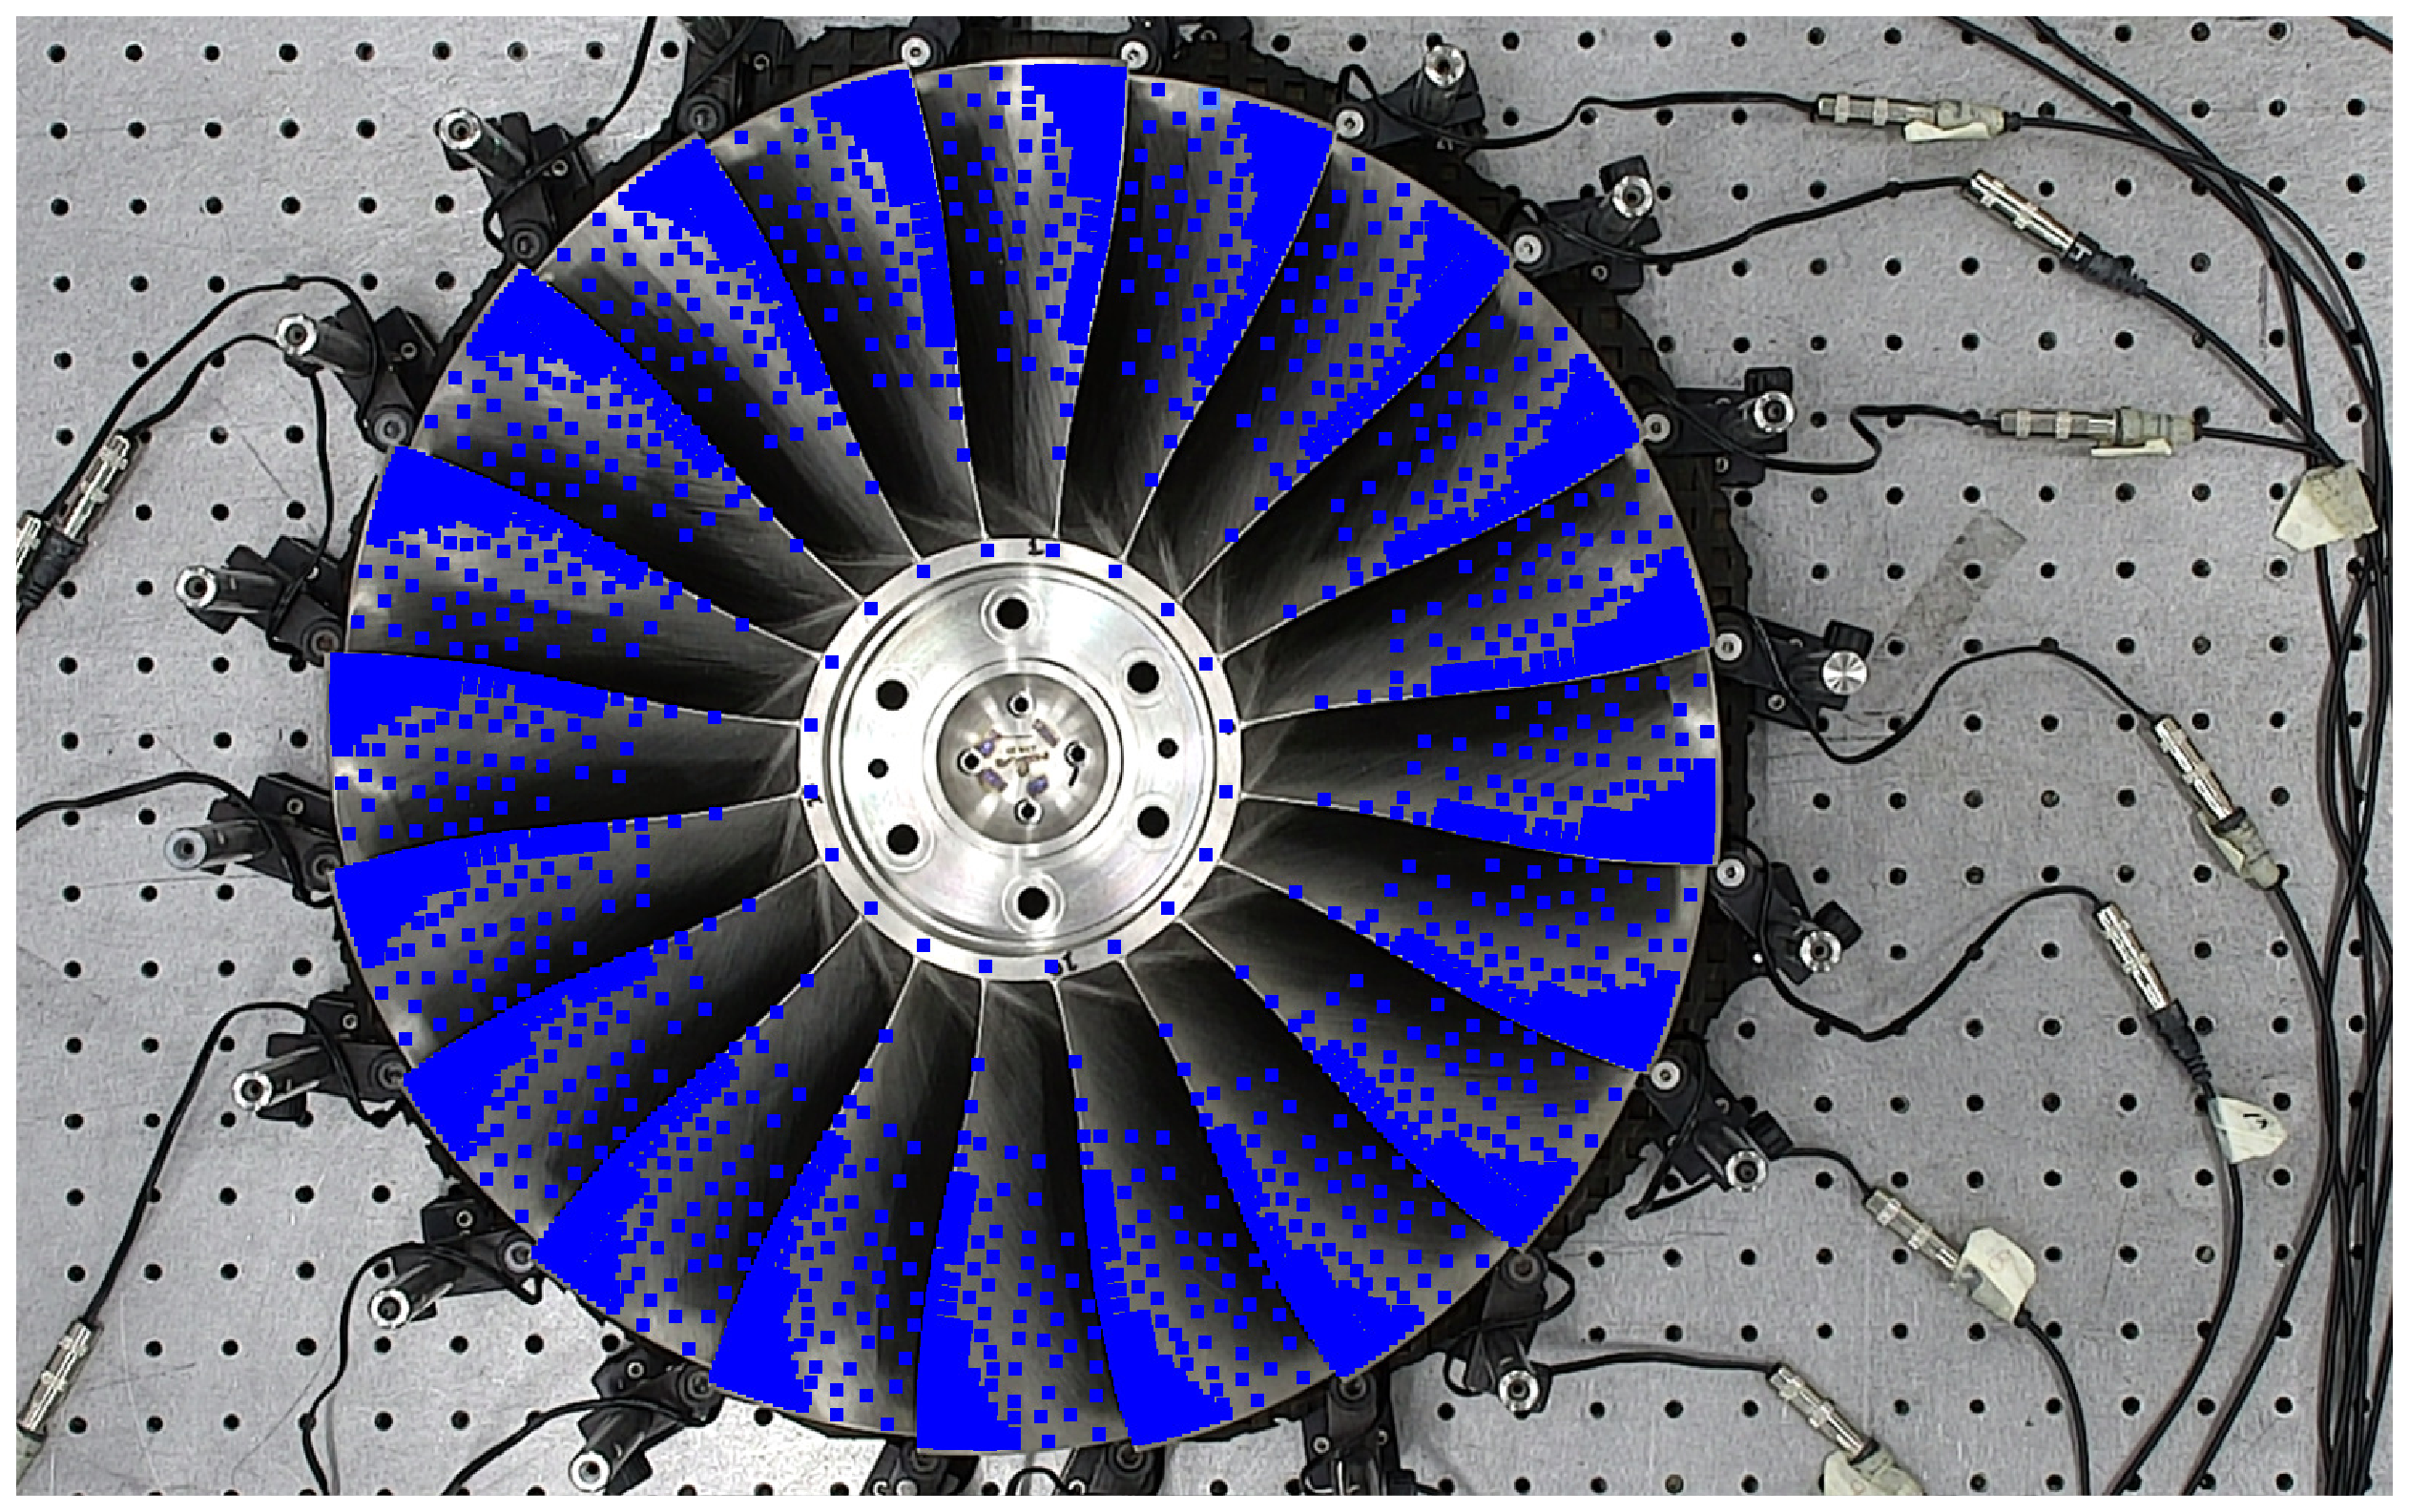
\includegraphics[width=\linewidth, alt = {TWE setup with scan points}]{figures/Figure4.eps}
    \caption{TWE setup with scan points}
    \label{fig:twe-setup}
\end{figure}

The rotor was excited at EOs 5 and 7 between 500~Hz and 10~kHz, targeting the first 17 mode families of the rotor. The experimental vibrational response was collected using a Polytec PSV QTec scanning vibrometer with a DV-03 decoder for maximal noise rejection. For the purpose of OMA, the vibrational response was collected at 185 points per blade, with Figure \ref{fig:twe-setup} showing the TWE setup with all 3700 points for the full rotor. The points were placed non-uniformly to maximize the collection of the mode shape near the blade edge and tip, where complex mode behavior was expected based on the FEA from the GMM. To reduce noise, three measurements per point were taken, and then complex-averaged at a frequency resolution of 0.38147 Hz. The full response of the rotor per EO resulted in a complex array sized $(24905, 185, 20)$, corresponding to 24,905 frequency samples, 185 points per blade, and 20 blades.

\subsection{Isolated Blade Vibration Testing}

While FMM ID is capable of accurately identifying sector mistuning deviations for blade-dominant mode families, modes with disk participation or non-isolated modes with frequency range overlap are more difficult to accurately characterize \cite{Feiner2004_2}. Furthermore, closely spaced mode families, with potential mode coupling and swapping as predicted by a preliminary modal analysis of the GMM, necessitate the collection of blade-alone responses for the validation of the GMM.

\begin{figure}
    \centering
    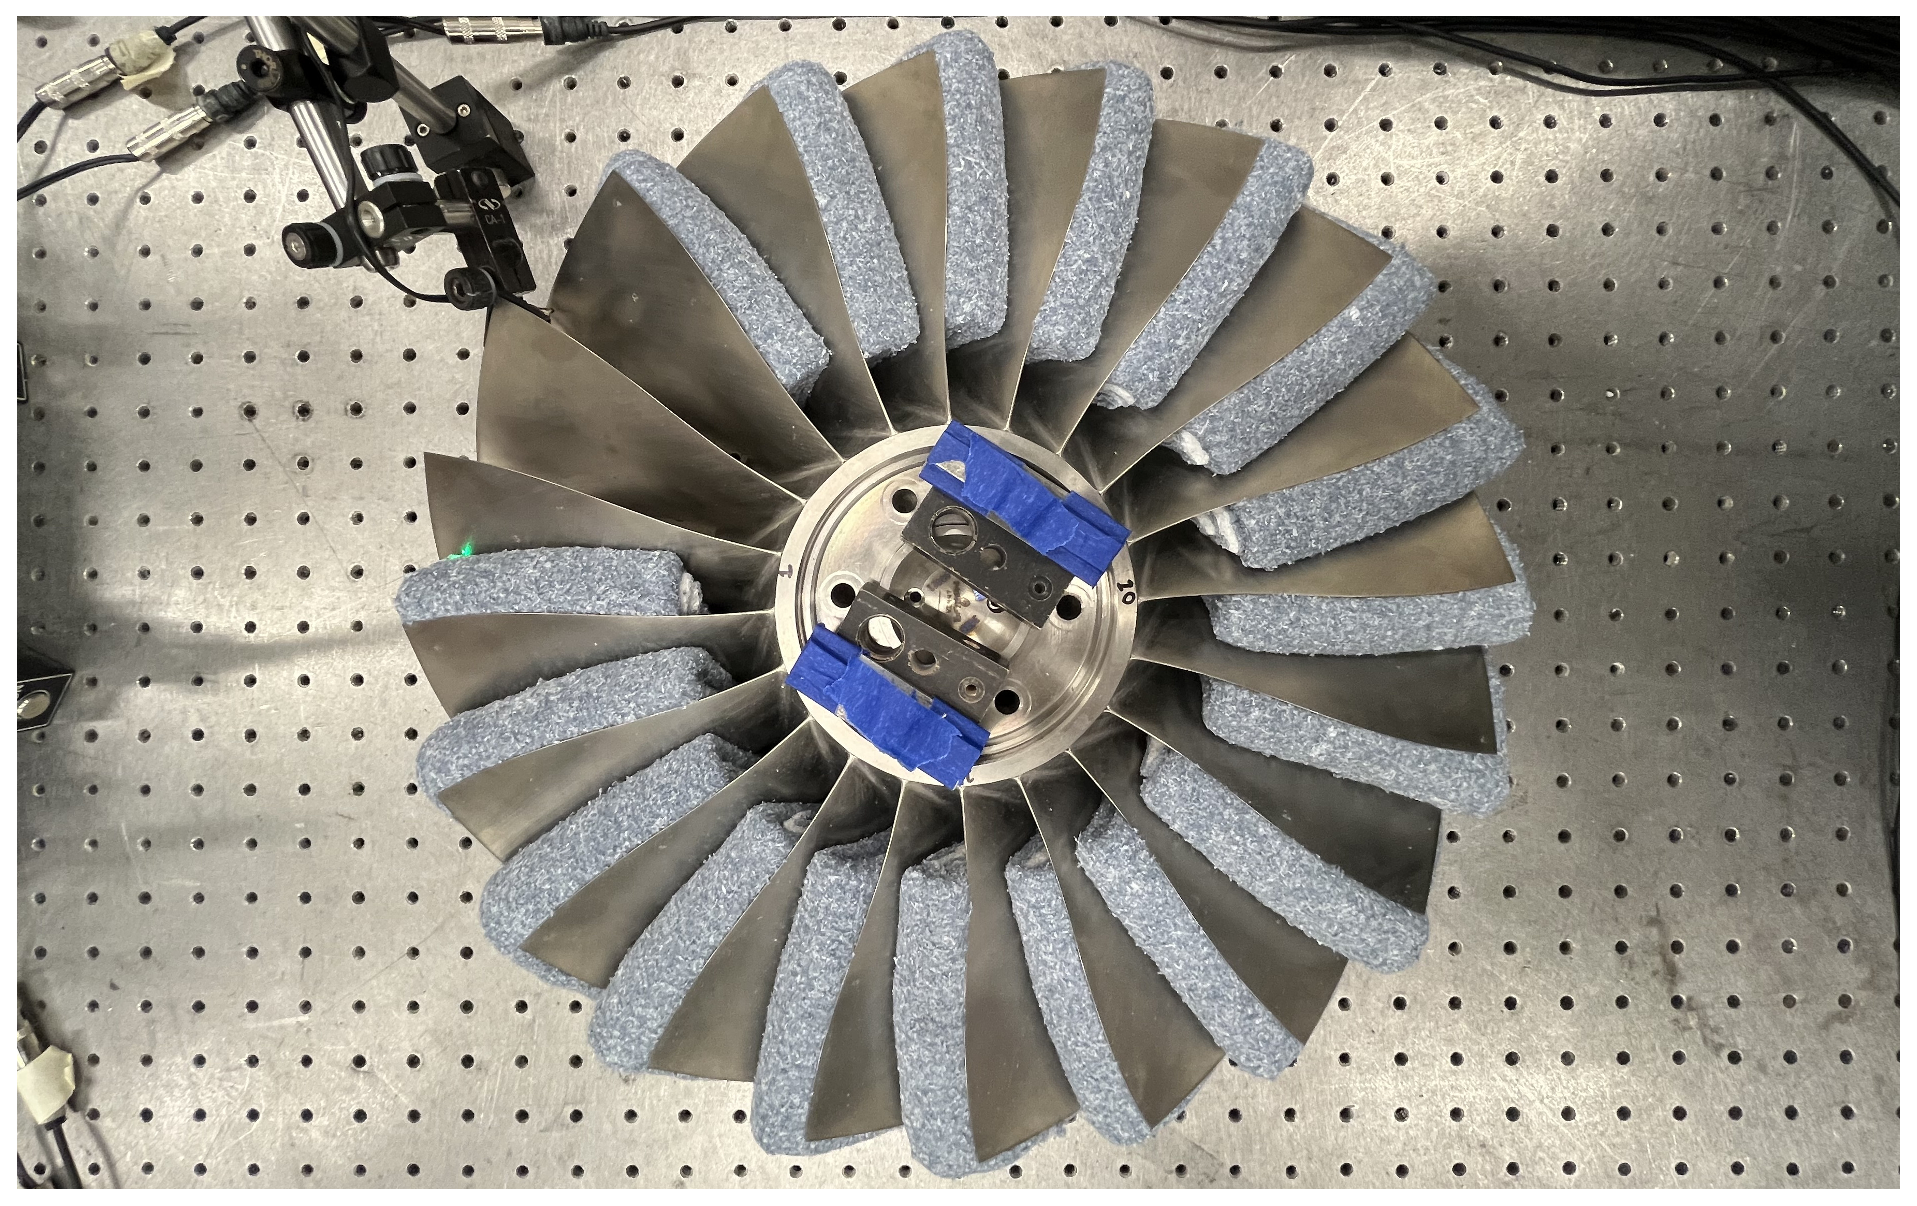
\includegraphics[width=\linewidth, alt = {Isolated blade response and pLSRA}]{figures/Figure5.eps}
    \caption{Isolated blade excitation setup}
    \label{fig:exp-isolated-setup}
\end{figure}

Figure \ref{fig:exp-isolated-setup} shows the isolated blade setup with single speaker excitation. During data collection, it was discovered that mass loading or blade damping alone was insufficient to fully isolate the blades. Additionally, the rotor was prone to shift when adjusting the unloaded and undamped blade. The most isolated and consistent response was achieved when the rotor was firmly clamped to the table, sound damping pads were placed between all but the excited blade, and the immediately adjacent blades were mass loaded. Mass loading was applied with two lead shot bags, which are not shown in Figure \ref{fig:exp-isolated-setup}. This approach proved robust enough to allow for the accurate and automated identification of closely spaced modes even with frequency separation between modes as small as 40~Hz. Figure \ref{fig:isolated-response} shows one such mode pair centered at 5.2~kHz, where mode swapping was expected to occur based on the GMM modal analysis. The figure shows both the actual and the predicted frequency response based on the automated mode identification via poly-reference least squares rational approximation (pLSRA) using pyFBS \cite{Bregar2022} and research from Guillaume et al.\ \cite{Guillaume2003}.

\begin{figure}[bp]
    \centering
    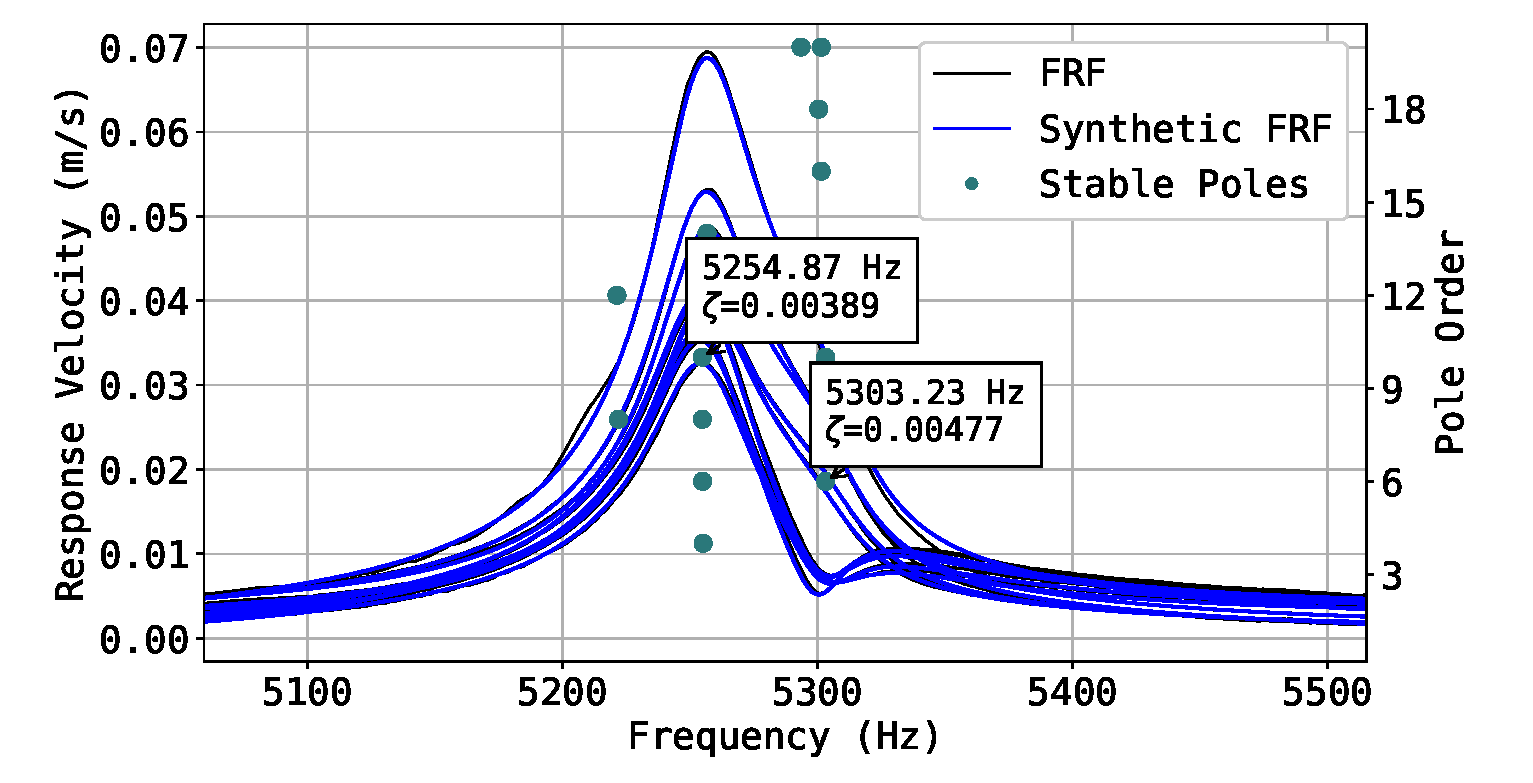
\includegraphics[width=\linewidth, alt = {Isolated Blade Response}]{figures/isolated-blade-response/Figure6.eps}
    \caption{Isolated blade response}
    \label{fig:isolated-response}
\end{figure}

pLSRA is used extensively in this research for modal parameter identification from the isolated blade complex frequency response. For a system with $n_i$ measurement points, the complex frequency response function (FRF) is denoted as

\begin{equation}\label{eq:frf_matrix}
    \mathbf{H}(\omega) =
    \begin{bmatrix}
        H_1(\omega_1)     & \dots  & H_1(\omega_{n_\omega})     \\
        \vdots            & \ddots & \vdots                     \\
        H_{n_i}(\omega_1) & \dots  & H_{n_i}(\omega_{n_\omega})
    \end{bmatrix},
\end{equation}

\noindent
where $\omega_k$ are the excitation frequencies. In the iterative pLSRA implementation used for this research, the FRFs for each point are approximated using a common denominator rational function:

\begin{equation}\label{eq:rat_approx}
    H_i(\omega) \approx \frac{N_i(j\omega)}{D(j\omega)}, \quad i=1,\dots,n_i,
\end{equation}

\noindent
with

\begin{equation}\label{eq:denominator}
    D(s) = s^{n_p} + a_{n_p-1} s^{n_p-1} + \dots + a_1 s + a_0, \quad s = j\omega,
\end{equation}

\begin{equation}\label{eq:numerator}
    N_i(s) = b_{i,n_p-1} s^{n_p-1} + \dots + b_{i,0}.
\end{equation}

\noindent
The poles of the system, $s_k$, are obtained from the roots of the denominator polynomial:

\begin{equation}\label{eq:poles}
    D(s_k) = 0, \quad k=1,\dots,n_p,
\end{equation}

\noindent
from which the natural frequencies $\omega_{n,k}$ and damping ratios $\zeta_k$ are calculated as

\begin{equation}\label{eq:freq_damp}
    \omega_{n,k} = |s_k|, \quad \zeta_k = -\frac{\Re(s_k)}{|s_k|}.
\end{equation}

\noindent
The mode shapes at each measurement point are proportional to the numerator evaluated at the poles:

\begin{equation}\label{eq:mode_shapes}
    \phi_{ik} = N_i(s_k),
\end{equation}

\noindent
and the mode participation factors are derived from the dominant singular vector of the numerator matrix evaluated at the poles, which for this research was assumed to be unity. The stability of the identified poles across multiple orders was determined from

\begin{equation}\label{eq:stab_criteria}
    \begin{aligned}
        |f_{n_p} - f_{n_{p+1}}|         & < \text{stab\_f}, \\
        |\zeta_{n_p} - \zeta_{n_{p+1}}| & < \text{stab\_d}, \\
    \end{aligned}
\end{equation}

\noindent
where only poles satisfying these conditions are considered stable, as their natural frequency and damping ratios do not change as the order of the polynomial increases. These stable poles were retained for OMA with the stability parameters tuned on a system-by-system basis. The iterative solver minimizes the frequency-domain least-squares error:

\begin{equation}\label{eq:lsq_error}
    \min_{a,b} \sum_{i=1}^{n_i} \sum_{k=1}^{n_\omega} \Big| H_i(j\omega_k) - \frac{N_i(j\omega_k)}{D(j\omega_k)} \Big|^2
\end{equation}

\noindent
to simultaneously identify the numerator and denominator polynomials across all measurement points.

Figure \ref{fig:isolated-response} shows the result of the automated application of pLSRA by selecting all of the identified stable poles and then iteratively removing duplicate poles based on mode shapes. The duplicate poles were identified and removed by selecting the pole with the highest modal assurance criteria (MAC) above a threshold of $0.9$ as calculated by:

\begin{equation}\label{eq:mac}
    \text{MAC}(\boldsymbol{\phi}_a, \boldsymbol{\phi}_b) = \frac{ \big| \boldsymbol{\phi}_a^\mathrm{H} \boldsymbol{\phi}_b \big|^2 }{ \big( \boldsymbol{\phi}_a^\mathrm{H} \boldsymbol{\phi}_a \big) \big( \boldsymbol{\phi}_b^\mathrm{H} \boldsymbol{\phi}_b \big) },
\end{equation}

\noindent
where $\boldsymbol{\phi}_a^\mathrm{H}$ denotes the conjugate transpose of $\boldsymbol{\phi}_a$. A MAC value of 1 indicates identical mode shapes, while 0 indicates orthogonal mode shapes.

The mode shapes used for the above comparison were calculated via the least-squares frequency domain (LSFD) method used by Guillaume et al.\ \cite{Guillaume2003}, which, for the sake of brevity, were calculated via

\begin{equation}\label{eq:lsfd}
    \mathbf{Y} = \mathbf{P} \, \mathbf{O},
\end{equation}

\noindent
where $\mathbf{Y}$ contains the real and imaginary parts of the measured FRFs, $\mathbf{P}$ is the frequency-dependent modal matrix constructed from the identified poles and participation factors, and $\mathbf{O}$ contains the complex modal constants corresponding to the mode shapes and residuals.

To automate the identification of modes in the isolated blade OMA, poles whose associated mode shapes yield $\text{MAC} > 0.9$ with a nearby pole are considered to be duplicates, and one of the poles is iteratively removed until only unique, stable poles remain. This proved robust, and the frequency response assurance criteria (FRAC) of the synthetic FRF generated via pLSRA exceeded 0.95 for the isolated blade response for all blades. The FRAC was calculated from the correlation between the magnitude of the measured FRF, $x = |\text{FRF}_\text{meas}|$, and the magnitude of the synthetic FRF, $y = |\text{FRF}_\text{syn}|$, defined as

\begin{equation}\label{eq:rac_pyfbs}
    \text{FRAC} = \frac{\sum (x - \bar{x})(y - \bar{y})}{\sqrt{\sum (x - \bar{x})^2} \, \sqrt{\sum (y - \bar{y})^2}},
\end{equation}

\noindent
where $\bar{x}$ and $\bar{y}$ are the mean values of $x$ and $y$, respectively. FRAC ranges from $0.0$ to $1.0$, with $1.0$ indicating perfect agreement between the synthetic and as-measured FRFs, and 0.0 indicating non-correlation. In practice, values above $0.7$ denote strong agreement with the FRF. Note that pLSRA proved to be robust for both isolated OMA as well as when applied to the full rotor, despite the closely spaced modes common in a full mistuned system. This will be discussed in detail in the results section, but the main finding is that a high number of observation points is critical when performing OMA on several closely spaced modes.

\section{As-manufactured Model Setup}

The parametric nature of the PBS rotors allows for a single common cyclic FEM to be used across the multiple rotor designs. An existing PBS Rotor 4 sector model from \cite{Gillaugh2018, Gillaugh2019} was modified by FEMORPH to match the as-measured geometry point cloud using the following procedure:

\begin{itemize}
    \item Load the FEM sector model and generate a full rotor from the single sector.
    \item Load the surface scan of the rotor.
    \item Globally register the scan to the FEM and align the rotor clocking.
    \item Perform Anderson accelerated ICP to align the scan to rotor geometry.
    \item Update the blade and disk geometry to match the surface geometry using FEMORPH.
    \item Make FEM cyclically symmetric.
    \item Repeat the ICP local surface registration and update the surface geometry again.
    \item Export updated node coordinates of the full rotor for downstream analysis.
\end{itemize}

\begin{figure}
    \centering
    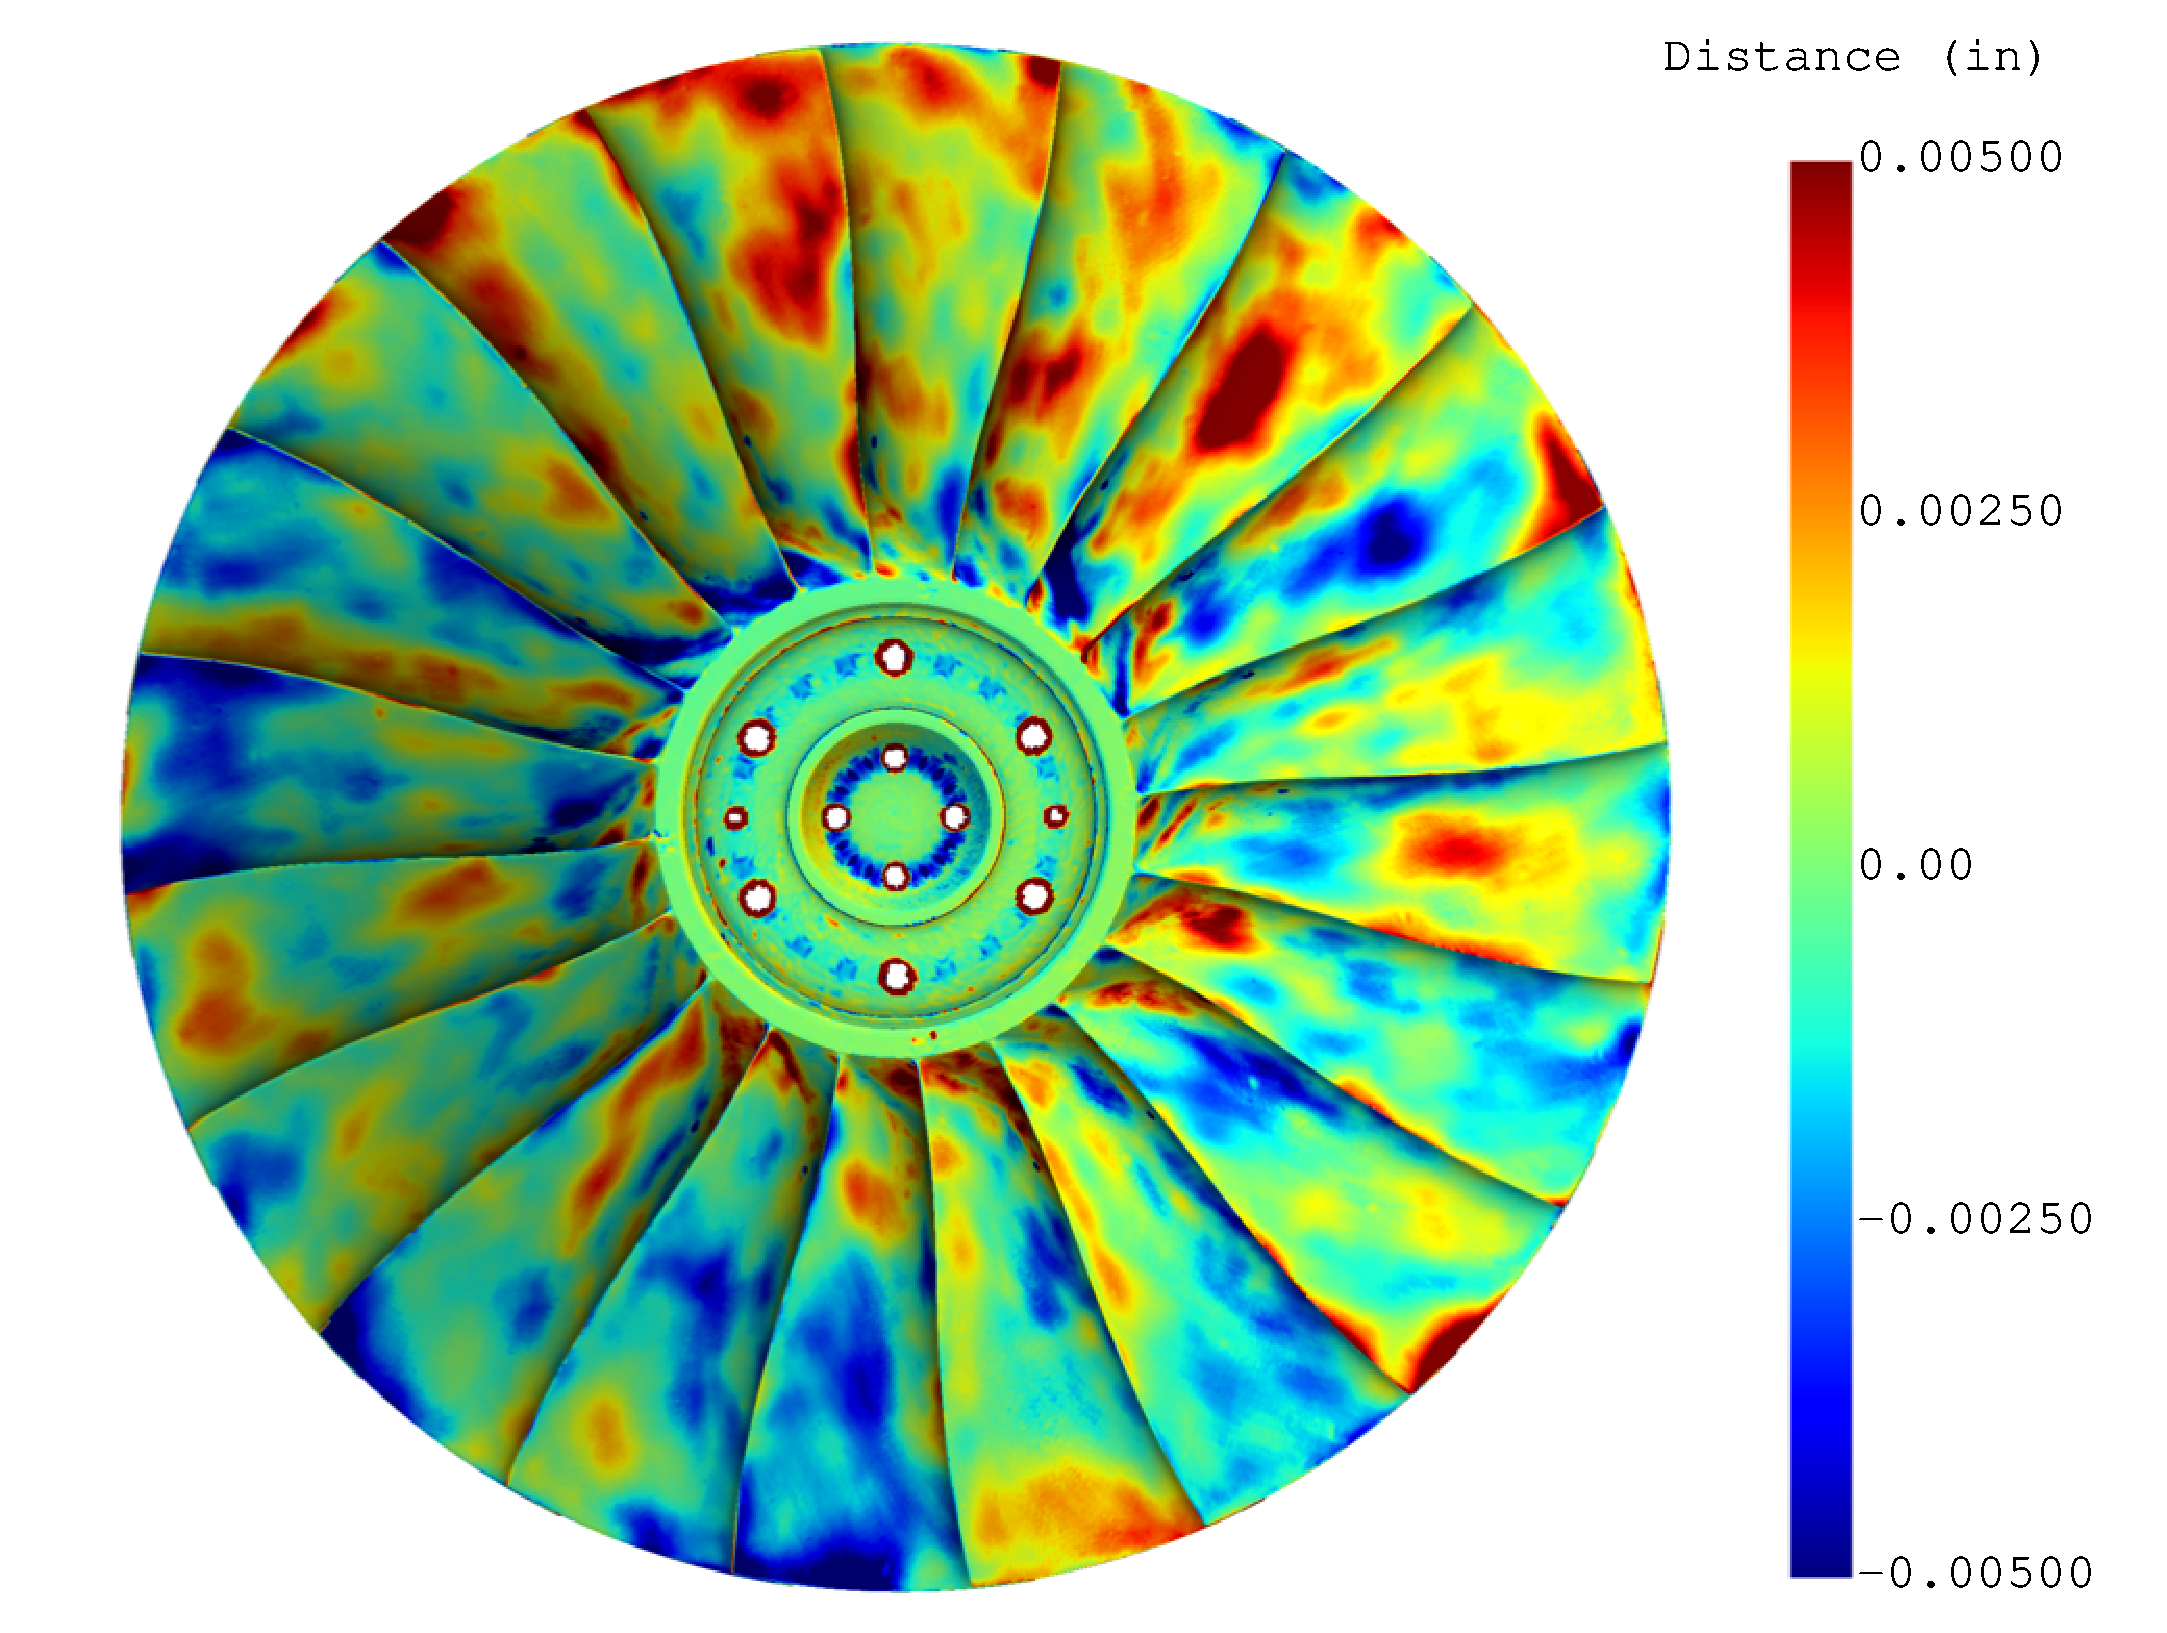
\includegraphics[width=\linewidth, trim=0 0 40 0, clip, alt = {Mean GMM to Surface Scan}]{figures/deviation-from-mean/Figure7.eps}
    \caption{Mean GMM to surface scan}
    \label{fig:gmm-to-surface}
\end{figure}

The distance between the cyclically symmetric GMM and the surface scan is shown in Figure \ref{fig:gmm-to-surface}. The cyclically symmetric GMM is created from an average of the scan 6 airfoil measurements. The magnitude and pattern of these deviations are considered typical of blade-to-blade geometry variations.

A mesh convergence assessment was performed, and it was determined that 396,085 nodes per sector were sufficient for the investigated frequency range. After updating the FEM's geometry to the measured point cloud data, each individual sector model and the mean sector model were exported and then analyzed using Ansys MAPDL. A cyclic modal analysis at EO 10 was performed for each of the individual sectors to match the experimental isolated blade setup, while a full cyclic modal analysis at all EOs (inclusive) between EO 0 and 10 was completed for the mean sector model to generate the expected tuned system frequencies and mode shapes.

\section{Results}

This results section determines the effect of manufacturing deviations on the full and isolated blade mode shapes, sector mistuning deviations, and full rotor physical response of the PBS Rotor 5. Validation of the GMM will be accomplished by comparing the predicted mode shapes from isolated blade GMM and full rotor GMM analyses to the experimental isolated and full rotor system mode shapes. Furthermore, using the FMM ID, the sector mistuning deviations will be extracted from the full rotor model and compared to both the isolated GMM and experimental results to validate both FMM assumptions and the GMM's ability to predict isolated sector deviations. These comparisons will be used to quantify the GMM's accuracy in capturing both global modal behavior as well as isolated blade mode shape variation.

The FMM was used to provide a common basis of comparison across all three methods of analysis and to establish a consistent framework for evaluating the effect of mistuning on the modal response of the rotor. However, FMM assumes no disk participation or variance of mode shapes between the blades of a mode family, and it will be shown that this assumption does not hold true for all modes of this rotor, given both the experimental and analytical isolated sector response.

\begin{figure}
    \centering
    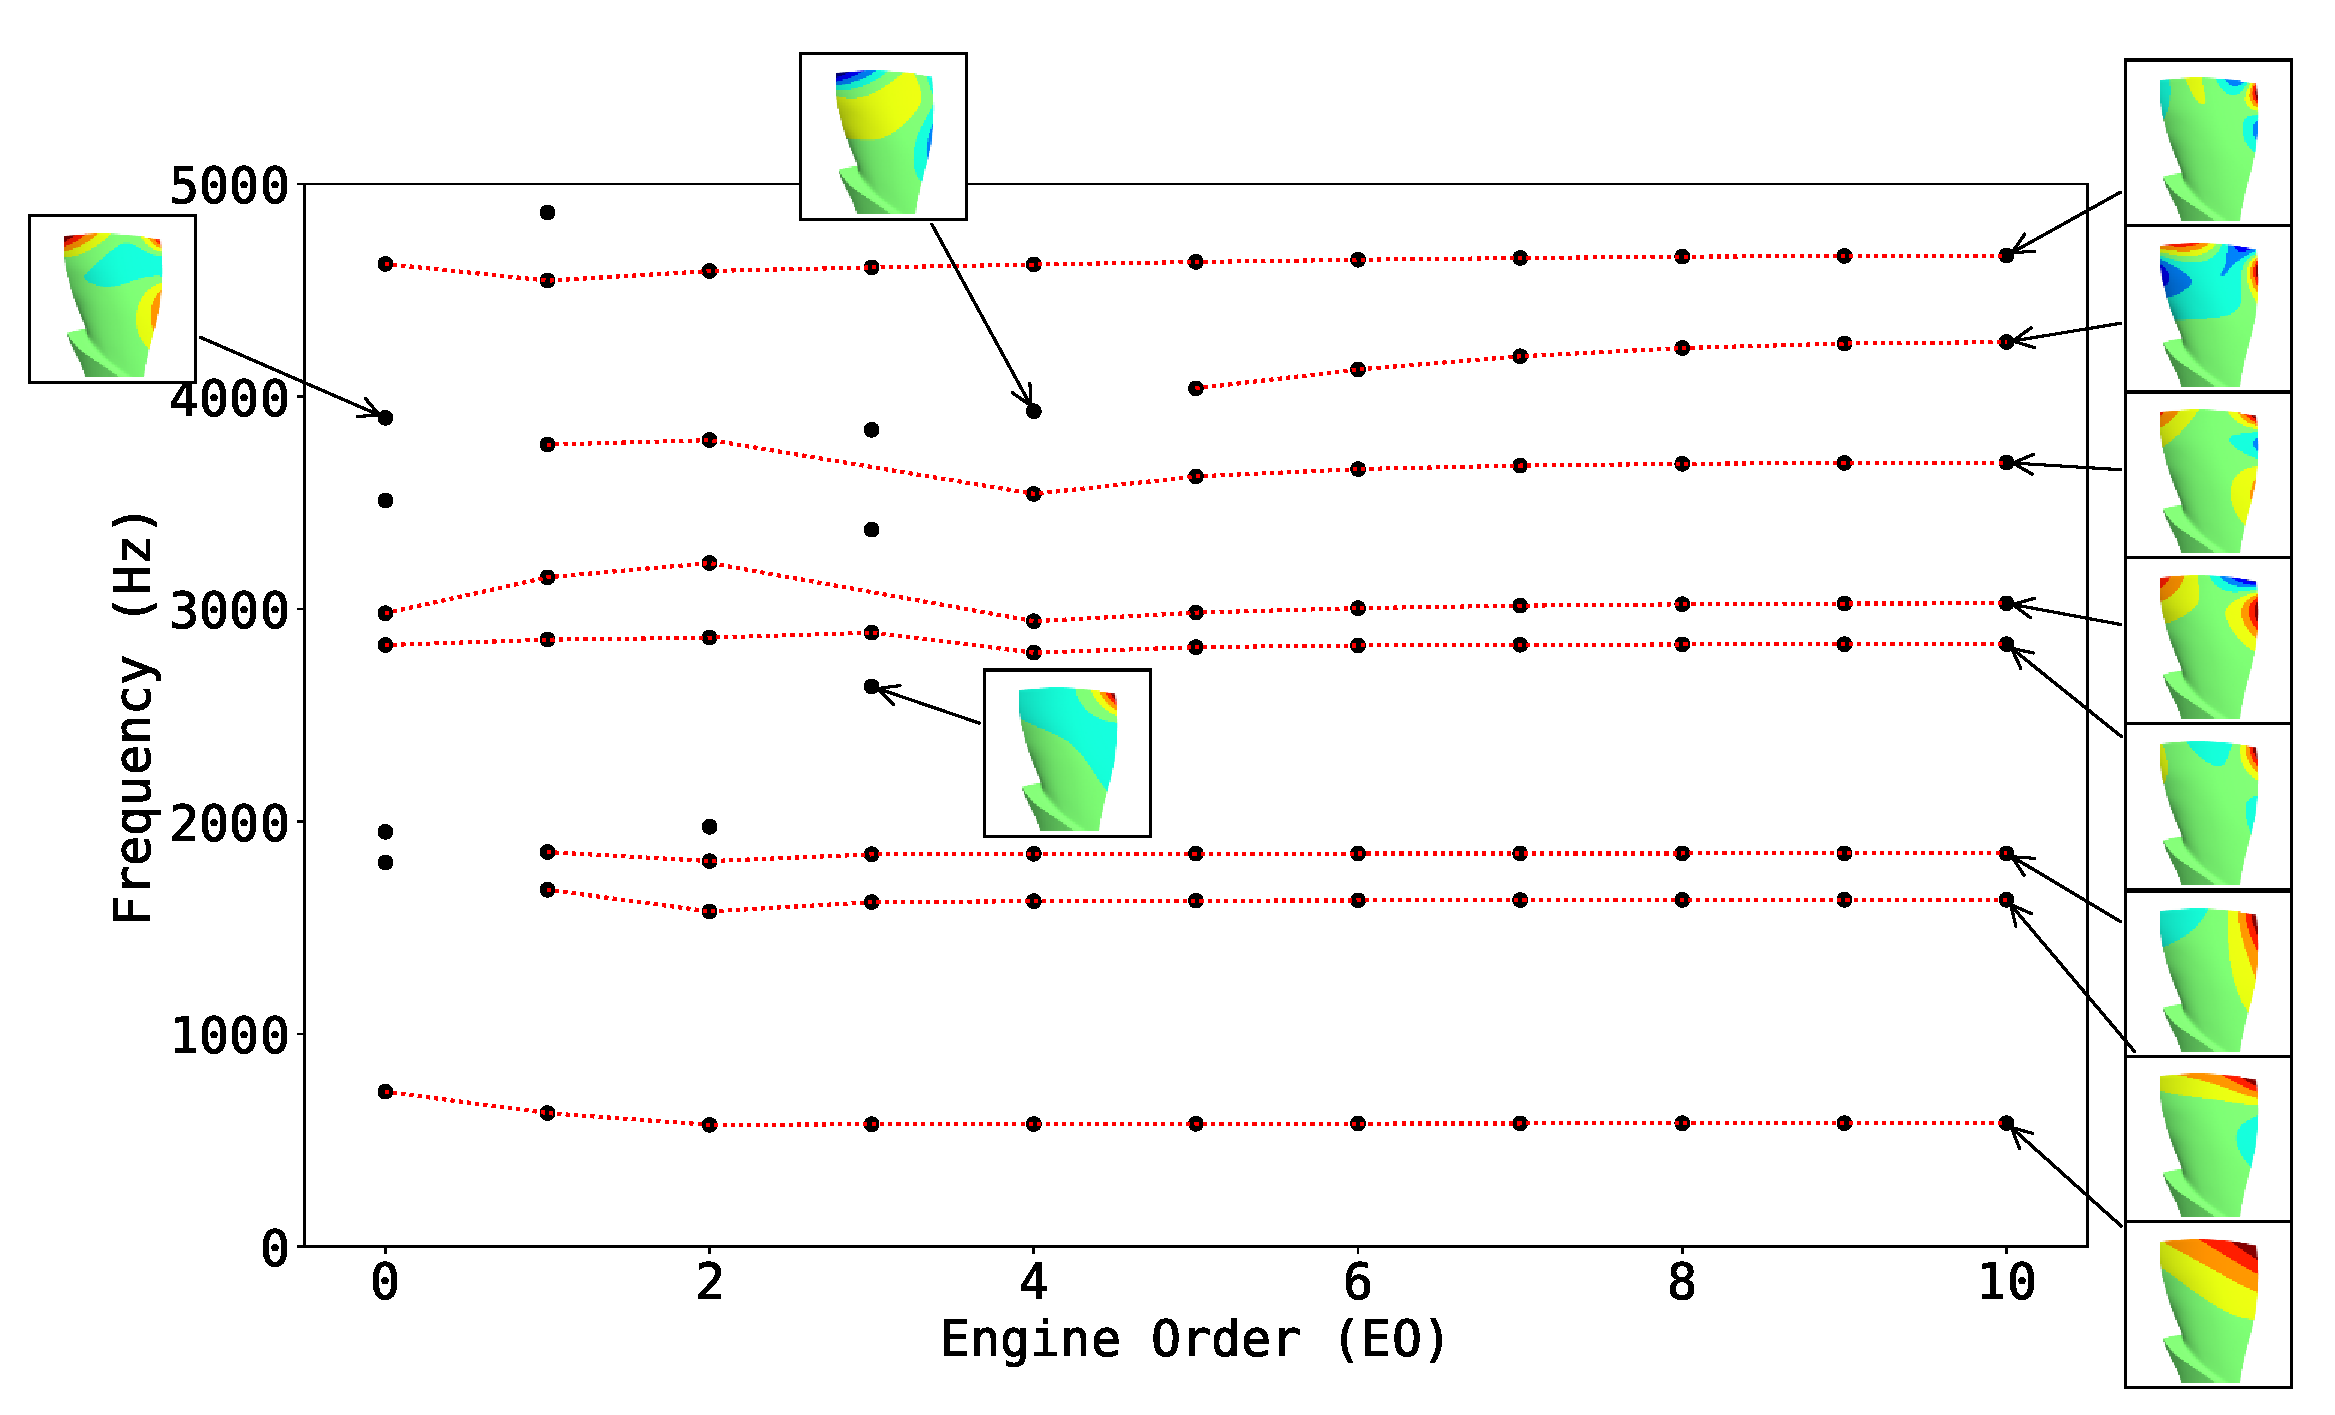
\includegraphics[width=\linewidth, alt = {GMM Nodal Diameter Plot (0.5--5 kHz)}]{figures/nd-plot-gmm/Figure8.eps}
    \caption{GMM nodal diameter plot (0.5--5~kHz)}
    \label{fig:nd-plot-0}
\end{figure}

Figures \ref{fig:nd-plot-0} and \ref{fig:nd-plot-1} show the nodal diameter plots generated from the tuned cyclic GMM. Each dot denotes a single tuned mode from the free-free cyclic analysis, while the dotted lines connect modes that share a mode shape with the highest EO based on a MAC of $0.7$. The highest EO mode was chosen as the ``anchor mode'', as this mode most closely resembles the isolated blade mode. Modes that fall outside this range are considered ``disk modes'' whose mode shapes are generally a mixture of two adjacent modes or a variation of a single adjacent mode. With the dual aim of this research to determine if mode shape variation and sector mistuning deviations can be predicted via a GMM due to blade-to-blade geometric variation, the first step is to validate the sector-to-sector mistuning deviations ($\Delta_\omega$) from a full rotor TWE test.

\begin{figure}[b]
    \centering
    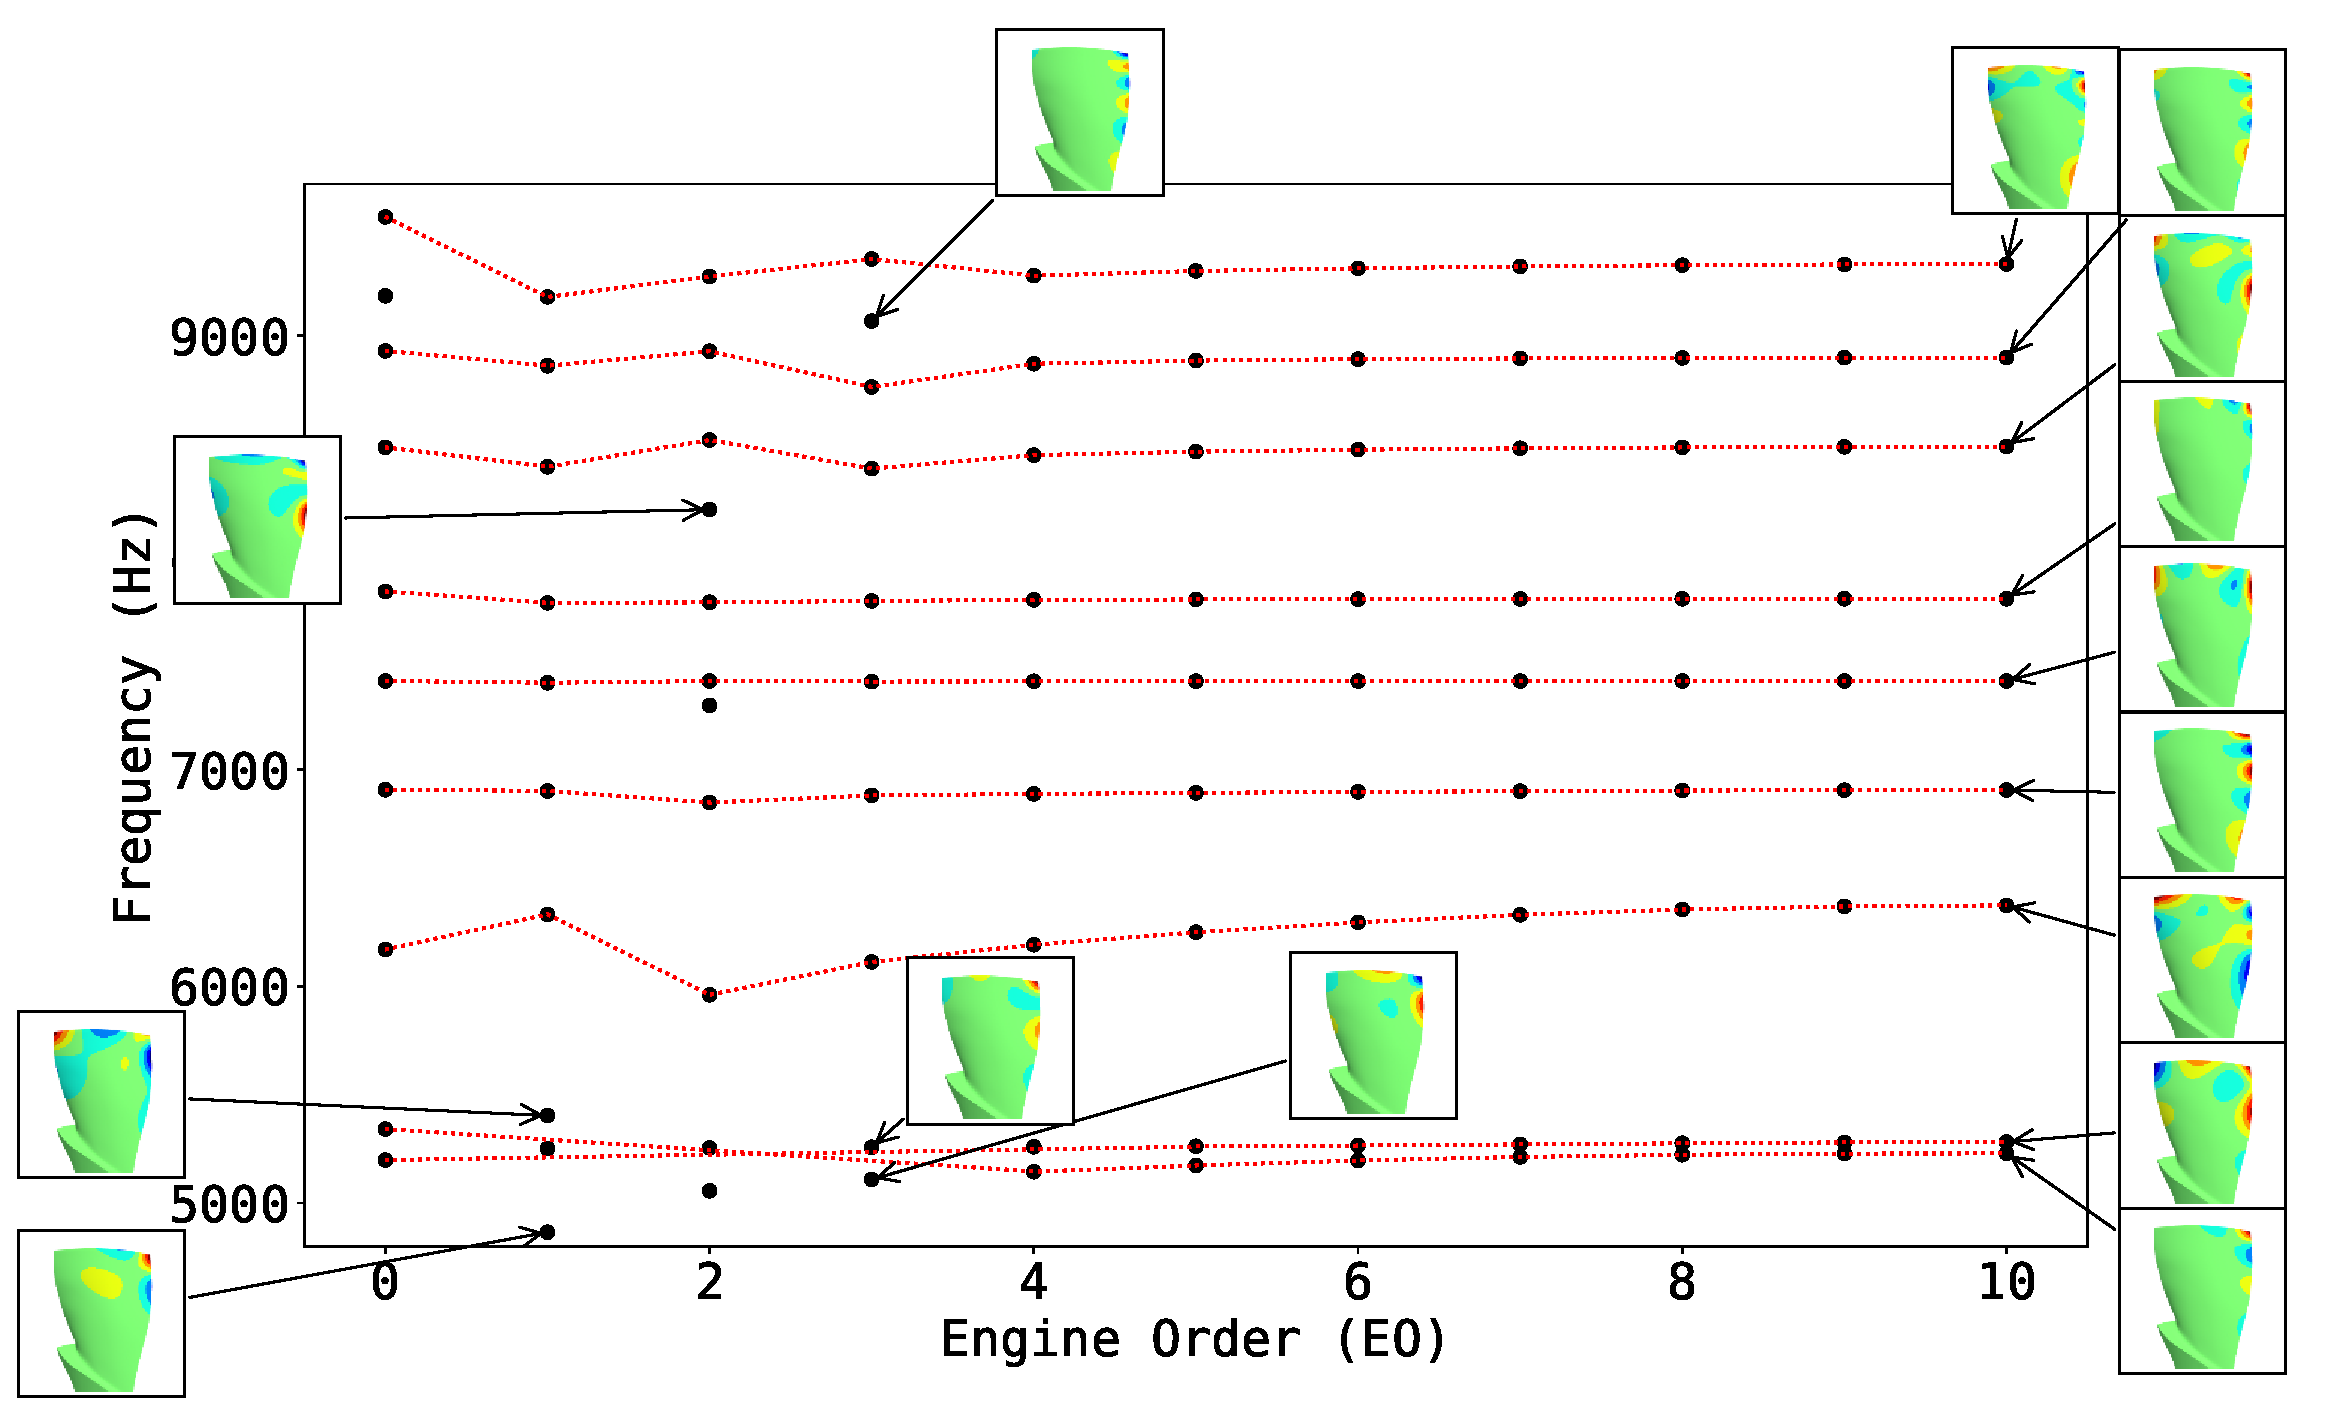
\includegraphics[width=\linewidth, alt = {GMM Nodal Diameter Plot (5--10~kHz)}]{figures/nd-plot-gmm/Figure9.eps}
    \caption{GMM nodal diameter plot (5--10~kHz)}
    \label{fig:nd-plot-1}
\end{figure}

The full rotor experimental results contained 17 modes within the 0.5--10 kHz frequency range, matching the GMM. These modes were automatically identified by isolating mode families based on their agreement with a synthetic FMM system while sweeping across the FRF and using FRAC as an agreement criterion. Next, FMM ID was run independently on each of the 185 points to determine the best point to apply FMM ID to. This ensured that even closely spaced modes could be identified despite their proximity or overlap with adjacent modes. This approach was then validated by comparing the FMM sector mistuning deviation $\Delta_\omega$ to the isolated GMM $\Delta_\omega$ as summarized in the appendix Tables~\ref{tab:appendix-mode-comparison} and \ref{tab:appendix-fmm-std}. The mean correlation in sector mistuning deviations between the GMM and full rotor FMM ID was $0.9697$, indicating excellent agreement between the GMM and the modes extracted via FMM in terms of sector mistuning deviations. More critical was the agreement between the sector mistuning deviations calculated through sectors isolation.

Table \ref{tab:iso-exp-table} (at the end of the paper) shows the GMM and FMM ID agreement with the isolated modes as identified using pLSRA from the isolated sector setup described by Figure \ref{fig:exp-isolated-setup}. Due to the placement of the exciter speaker at the blade tip (and typically using only one speaker per blade), only 13 out of the 17 modes could be identified from the isolated blade response. However, all of the sector deviations from the 13 identified isolated modes strongly agreed with both GMM and FMM ID. The mean correlation between the GMM and isolated experimental results was $0.9874$, and between the FMM ID identified modes from the full model was $0.9828$, showing that, at least for these modes, both approaches correctly calculate the sector mistuning deviations of the rotor. Before comparing those modes with significant disk participation, it is useful to first validate FMM and the GMM on a single blade-dominant mode.

\begin{figure}[!b]
    \centering
    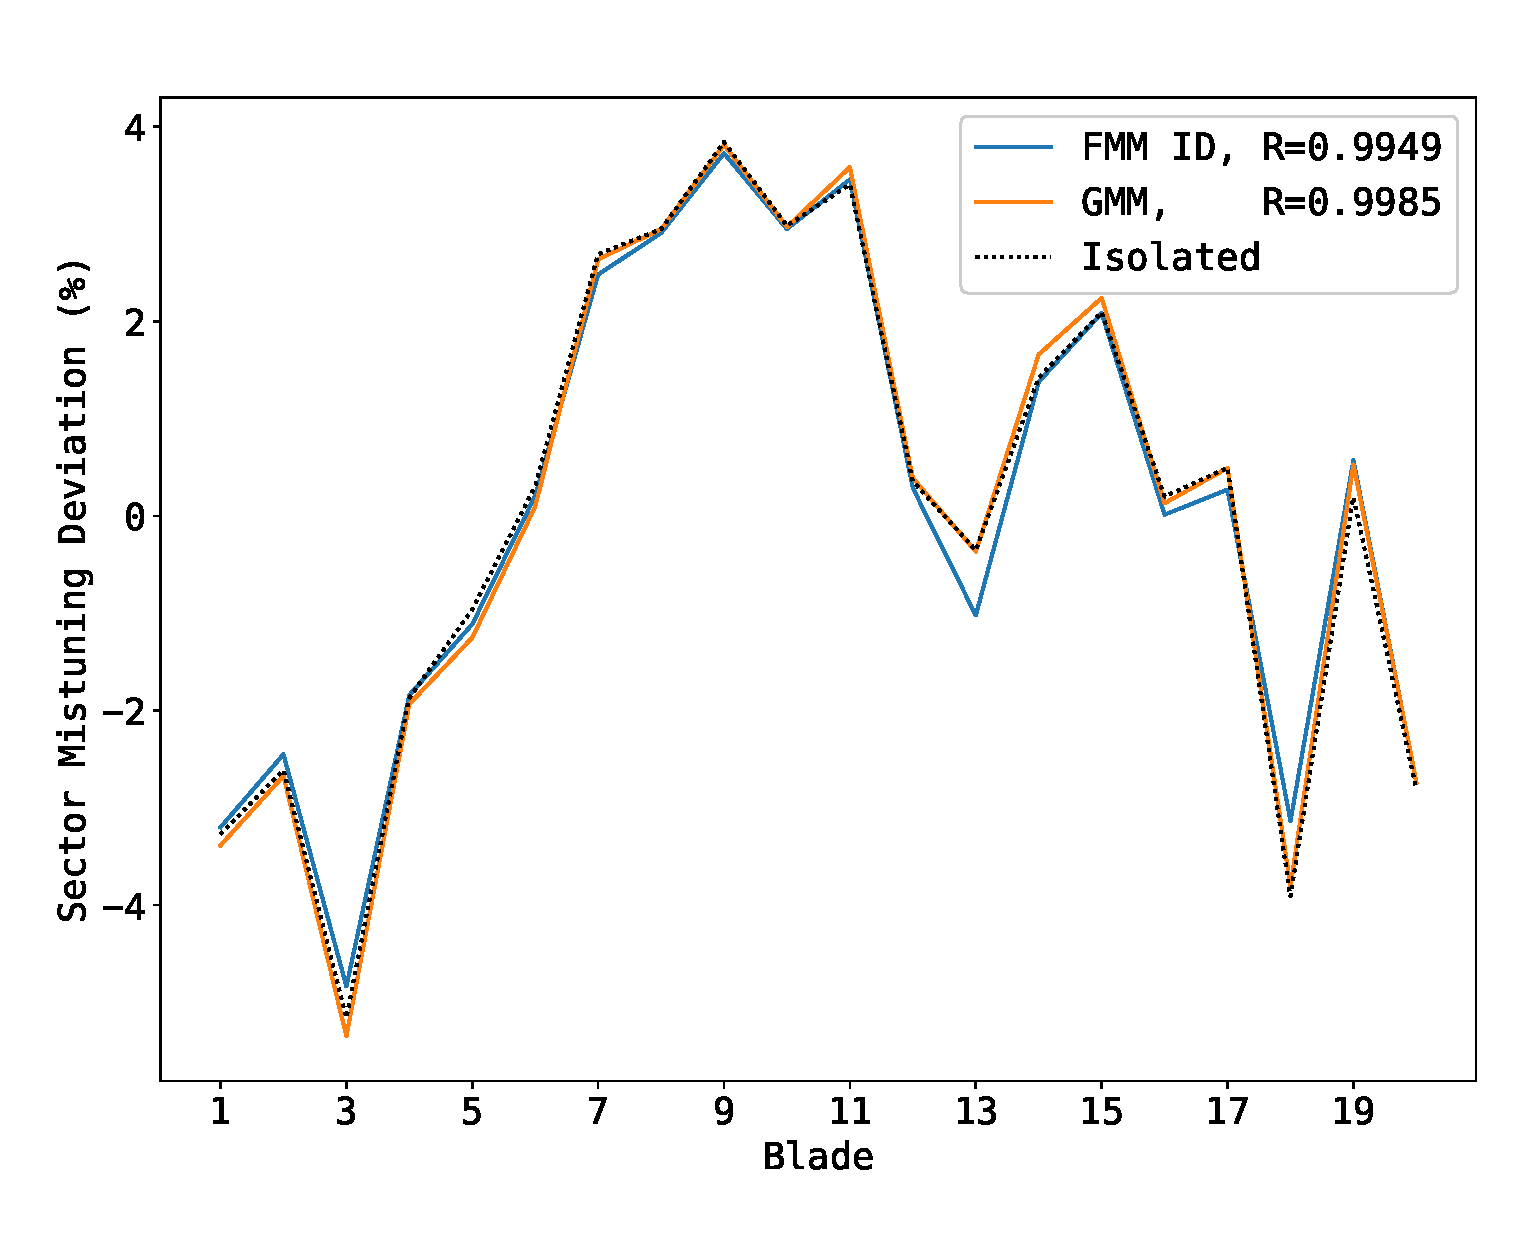
\includegraphics[width=\linewidth, trim=0 0 0 35, clip, alt = {Mode 14 Sector Mistuning Deviations}]{figures/auto-id-full/Figure10.eps}
    \caption{Sector mistuning deviations -- Mode 14}
    \label{fig:mode-14-dw}
\end{figure}

\begin{figure}
    \centering
    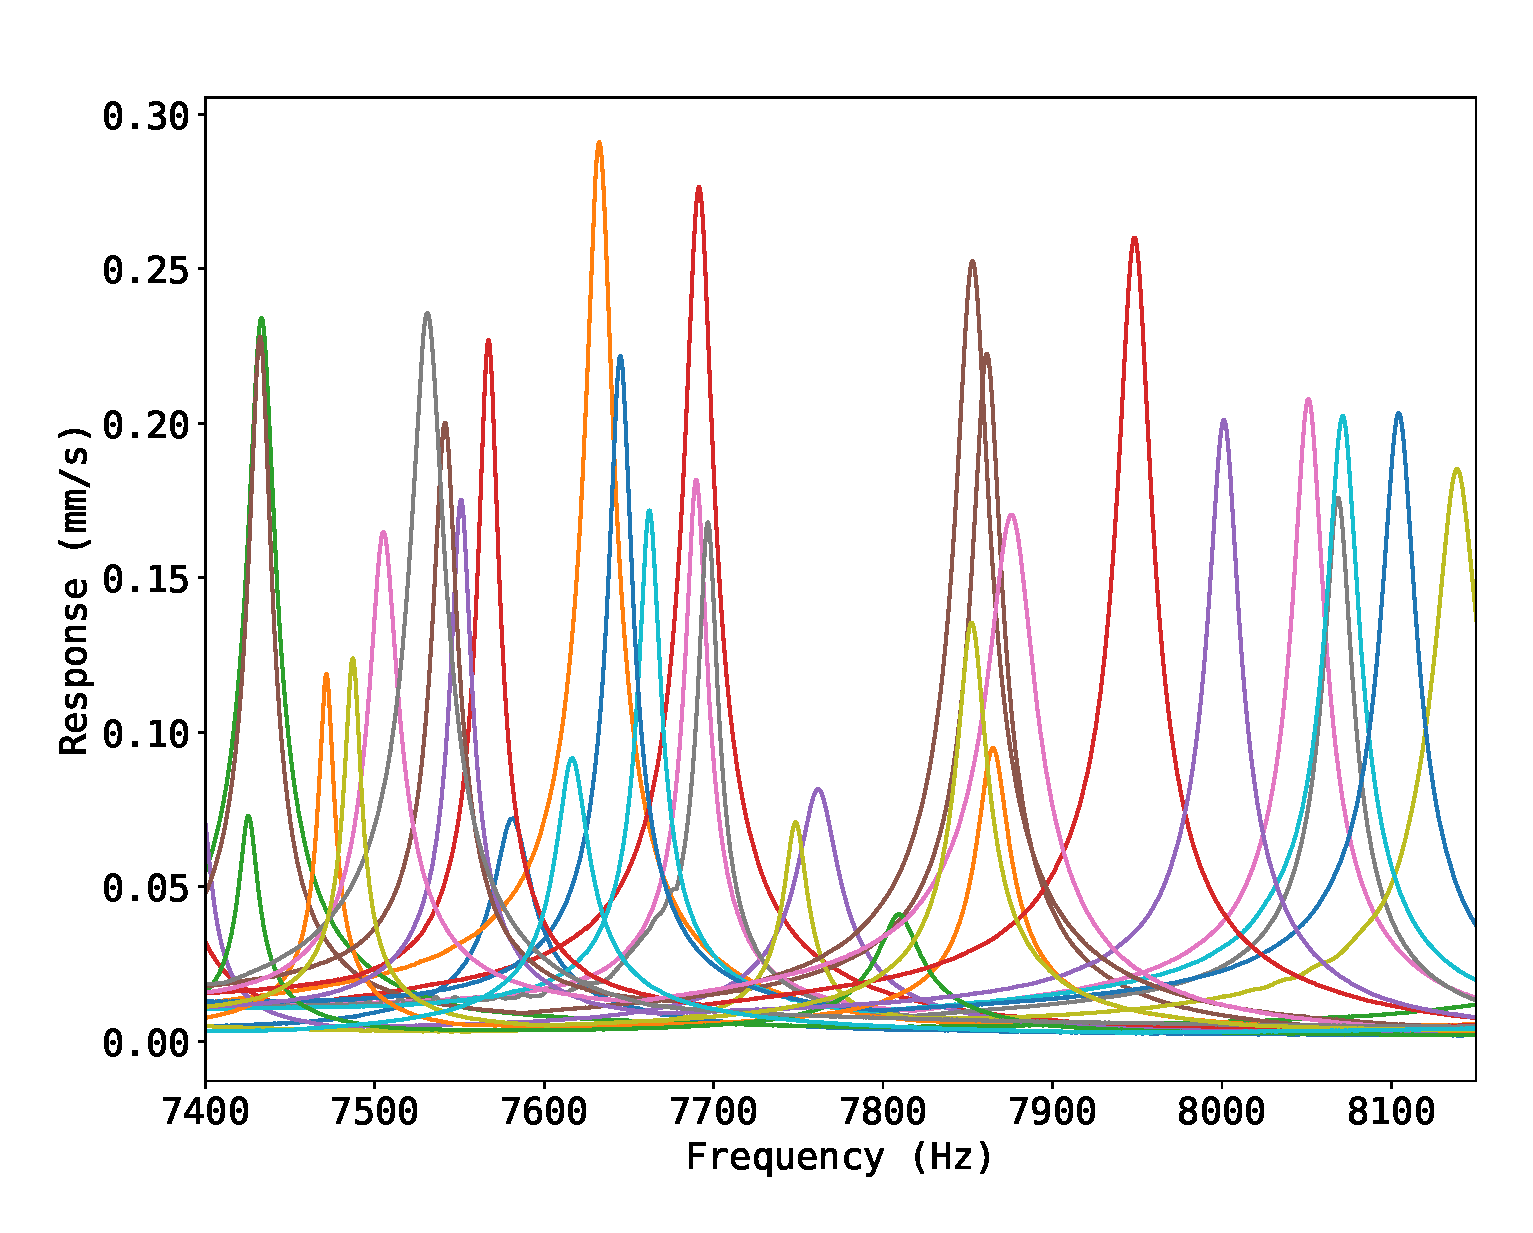
\includegraphics[width=\linewidth, trim=0 0 0 35, clip, alt = {Isolated Blade-Alone Experimental FRF - Mode 14}]{figures/auto-id-full/Figure11.eps}
    \caption{Isolated blade-alone experimental FRF -- mode 14}
    \label{fig:mode-14-frf-blades}
\end{figure}

Mode 14 shows strong agreement across all three datasets, with Figure \ref{fig:mode-14-dw} demonstrating that the sector mistuning deviations predicted by the FMM, GMM, and isolated experimental analyses are almost identical. This mode has minimal veering in its tuned system modes as calculated by FMM and the GMM, indicating that it is a blade-dominant mode with minimal disk participation, making it an excellent candidate for FMM. The sector mistuning deviations ($\Delta_\omega$) were calculated from FMM ID, experimentally obtained through blade isolation as shown in Figure \ref{fig:mode-14-frf-blades}, and analytically using isolated blade analysis at EO 10 since a free-free analysis at the highest EO resulted in a more accurate prediction of $\Delta_\omega$. Note that Figure \ref{fig:mode-14-frf-blades} contains more than 20 peaks, where the correct modes were identified from pLSRA via MAC matching, with non-matching modes reporting nearly orthogonal MACs ($0.0$). FMM operates under the assumption that mode shapes are invariant between blades, and while observations show minor variations in mode shapes, FMM still faithfully estimates $\Delta_\omega$ for this mode.

\begin{figure}[!b]
    \centering
    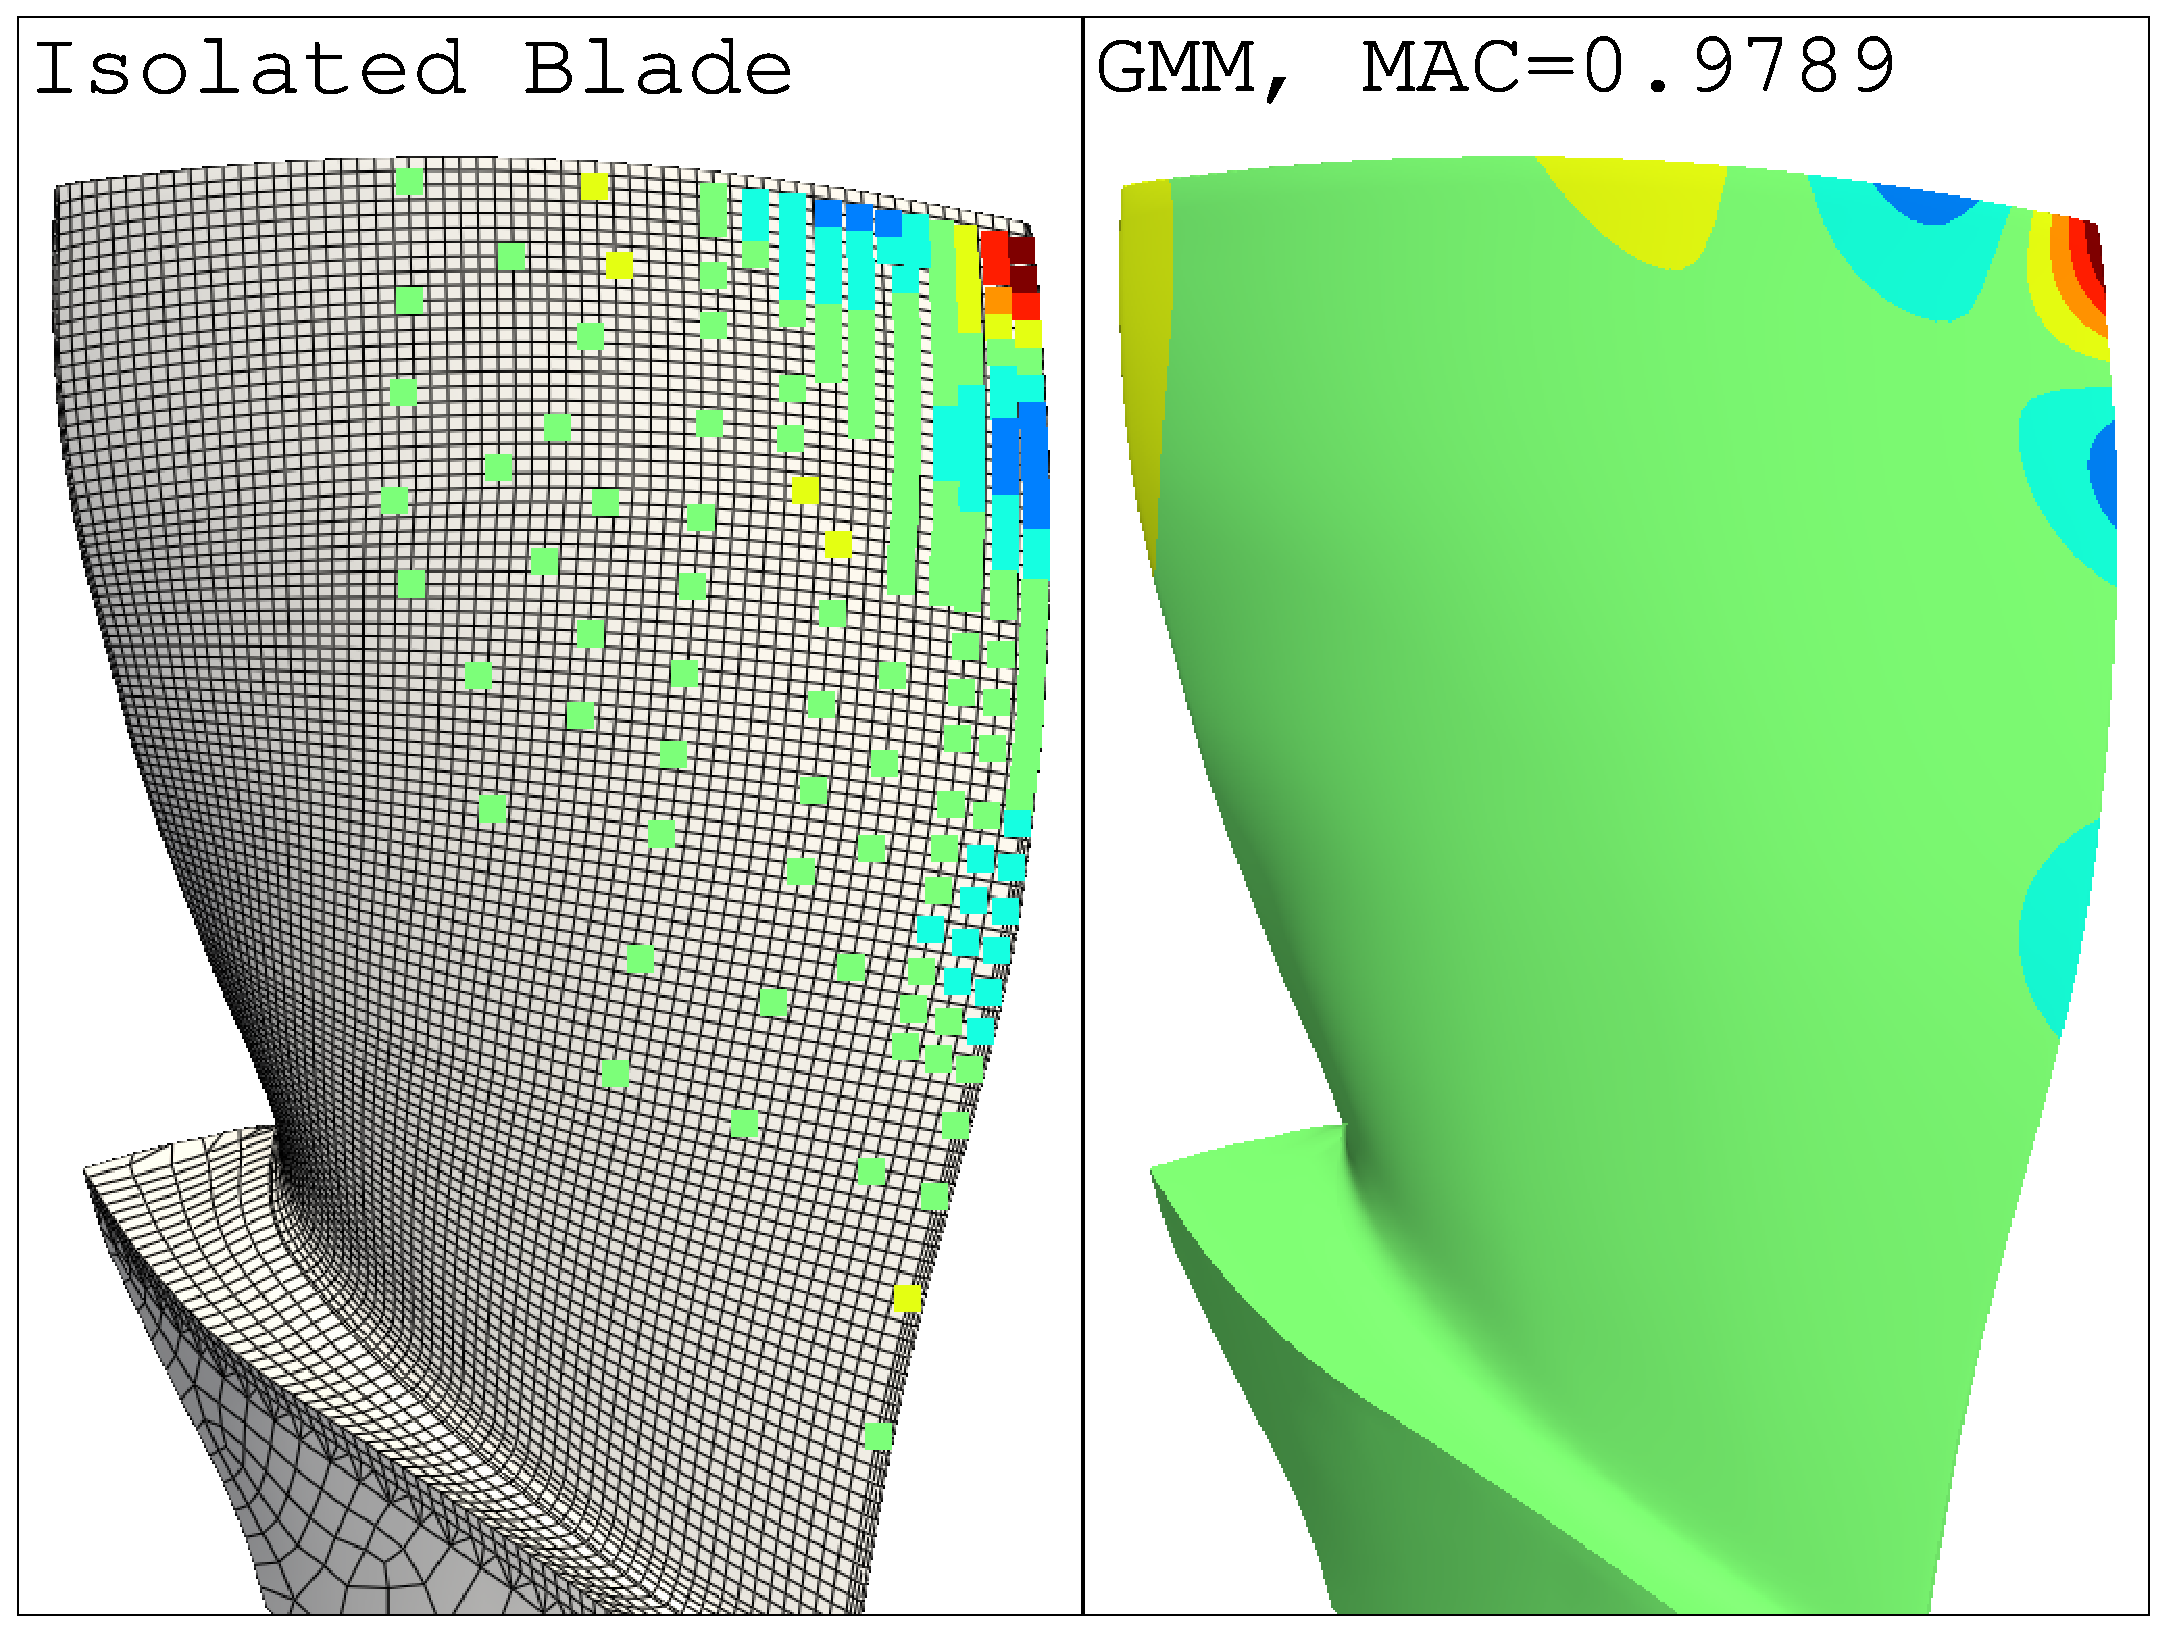
\includegraphics[width=\linewidth, alt = {Mode 14 - Mean Mode Shape}]{figures/auto-id-full/Figure12.eps}
    \caption{Mean mode shape comparison -- mode 14}
    \label{fig:mode-14-ms}
\end{figure}

Figure \ref{fig:mode-14-ms} shows the mode shape from mode 14 calculated from both the GMM and observed by the laser vibrometer in the isolated experiment. The mean mode shape from the GMM closely matches the mean mode shape of the experiment with a MAC of $0.9789$. One key question of this research is whether geometric variations can cause sector-to-sector mode shape variations, and this mode shows variation between both the analytically derived mode shapes from the GMM and from the isolated sector results. To determine the mode shape variation among a single mode, MACs were calculated between all blades within the single mode via Equation \ref{eq:mac}. In a rotor with zero mode shape variation, the entire matrix would be expected to be $1.0$, while a rotor with blade-to-blade geometric variation would have the mean of the upper triangle (excluding the diagonal) between $0.0$ and $1.0$, with a value less than $1.0$ indicating greater intra-blade mode shape variation. This value will be denoted as $\overline{\mathrm{MAC}}_{i<j}$ and defined by Equation \ref{eq:mac_upper}:

\begin{equation}\label{eq:mac_upper}
    \overline{\mathrm{MAC}}_{i<j} = \frac{2}{n(n-1)} \sum_{i<j}^{n} \mathrm{MAC}_{ij}
\end{equation}

\noindent
where $\mathrm{MAC}_{ij}$ corresponds to the MAC between blades ${i}$ and ${j}$ for a single mode, and ${n}$ is the number of blades in the rotor.

For this mode, the mean of the upper triangle of the blade-alone experimental response was $0.9348$, indicating there is some blade-to-blade mode shape variation. As for the GMM, the $\overline{\mathrm{MAC}}_{i<j}$ was $0.9643$, indicating that either the GMM predicts less mode shape variation, that there is experimental noise, or the mode shapes were not perfectly identified. Given the high mean mode shape agreement, it appears that experimental noise is the most likely reason given that the mode shapes can be compared favorably directly between each individual blade.

The third column in Table \ref{tab:iso-exp-table} shows the agreement along the diagonal of the MAC matrix between the GMM and pLSRA identified modes at common blades (i.e. GMM blade 1 and experimentally isolated blade 1). Unlike comparing across the upper triangle, by comparing the analytically predicted and observed mode shapes across the same blade indices, it can be determined if the mode shape variation is stochastic or deterministic when only modifying the geometry of the model. As shown in Table \ref{tab:iso-exp-table}, a value of $0.9702$ for $\overline{\mathrm{MAC}}_{i=j}$ for mode 14, which is both higher the value of $0.9230$ for $\overline{\mathrm{MAC}}_{i<j}$ and close to the mean mode shape MAC, indicates that geometry, and not experimental noise, plays a dominant role in mode shape variation. Furthermore, even for this blade-dominant mode family, mode shape variation is evident and can be predicted via a GMM. Figure \ref{fig:mode-14-all-ms-gmm}, in Appendix \ref{appendix:mode_shape_variation}, shows the variation for this mode from the GMM FEA, where significant variation is seen along the magnitudes of the leading edge modal deflections. This has a major implication regarding FMM: while FMM ID can accurately predict the sector-to-sector frequency variation, as it assumes consistent mode shapes between blades, it should have a greater error than the GMM when predicting sector mistuning variation. This is indeed the case, and referencing Figure \ref{fig:mode-14-dw}, the $\mathrm{MSE}$ of the FMM identification is $7.587\times10^{-6}$, four times greater than the GMM’s $\mathrm{MSE}$ of $2.167\times10^{-6}$, which is consistent with its slightly lower correlation ($r=0.9949$ versus $r=0.9985$) to the isolated blade experimental results. This demonstrates that the GMM can be used to predict both the mode shape variation and sector mistuning deviation for a blade-dominant mode family.

\subsection{Mode Swapping in the Isolated Blades}

\begin{figure}
    \centering
    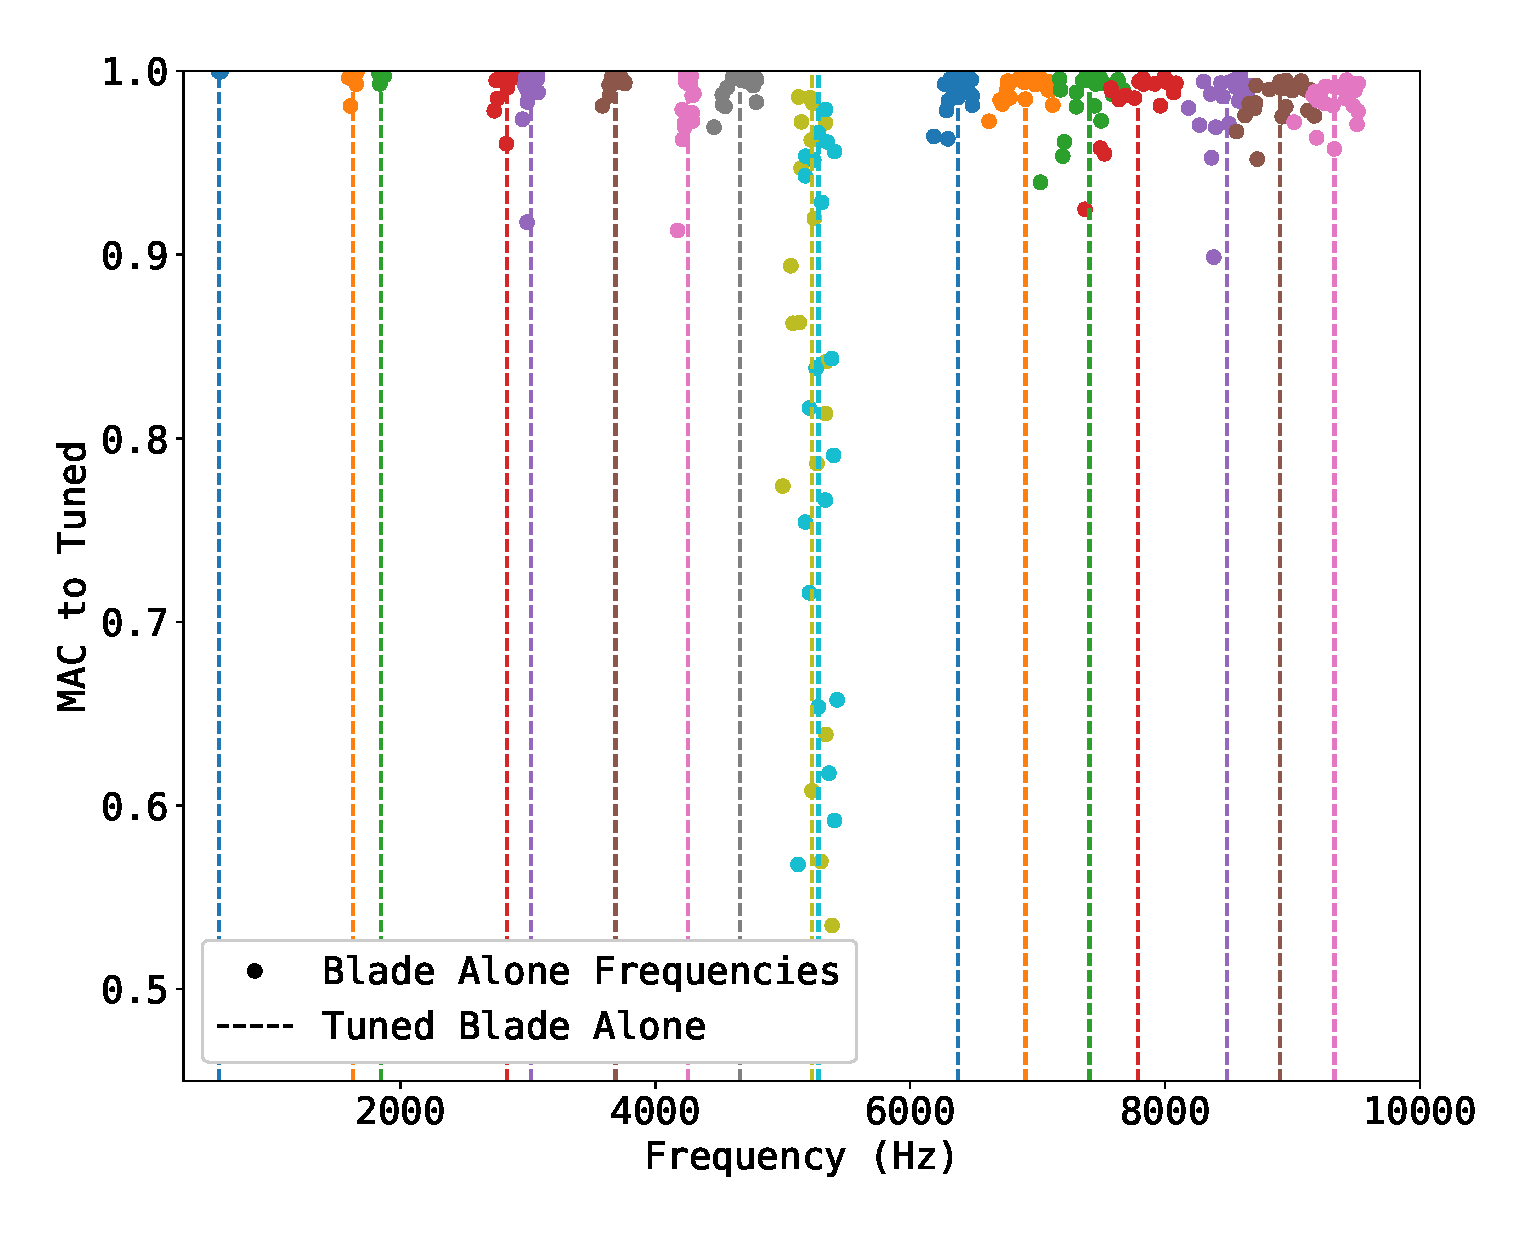
\includegraphics[width=\linewidth, alt = {GMM - Tuned to Mistuned MAC Variation}]{figures/mac-scatter/Figure13.eps}
    \caption{GMM -- tuned to mistuned MAC variation}
    \label{fig:mac-scatter}
\end{figure}

Not all modes shown in Table \ref{tab:iso-exp-table} are blade-dominant or have consistent isolated mode shapes. While the majority of the modes from Table \ref{tab:iso-exp-table} have mean upper triangle MAC scores ($\overline{\mathrm{MAC}}_{i<j}$) near or above $0.9$, 2 out of the 13 modes indicate significant mode shape variation. Modes 9 and 10 have a $\overline{\mathrm{MAC}}_{i<j}$ of $0.7071$ and $0.5737$ indicating that the mode shape varies widely between the experimentally obtained isolated blade mode shapes in a phenomenon known as mode swapping; where adjacent closely spaced mode shapes appear to exchange modal content between either individual blade modes or tuned modes. The GMM also predicts this phenomenon, and Figure \ref{fig:mac-scatter} shows that modes 9 and 10 both show substantial variation between their tuned mode shapes as calculated from the mean tuned sector analysis and their individual geometrically mistuned mode shapes. This scatter plot also shows strong agreement with Table \ref{tab:iso-exp-table}, where the first eight modes show very little variation between blades in their $\overline{\mathrm{MAC}}_{i<j}$ score and a strong MAC agreement between the tuned and mistuned mode shapes of the GMM.

\begin{figure}[b]
    \centering
    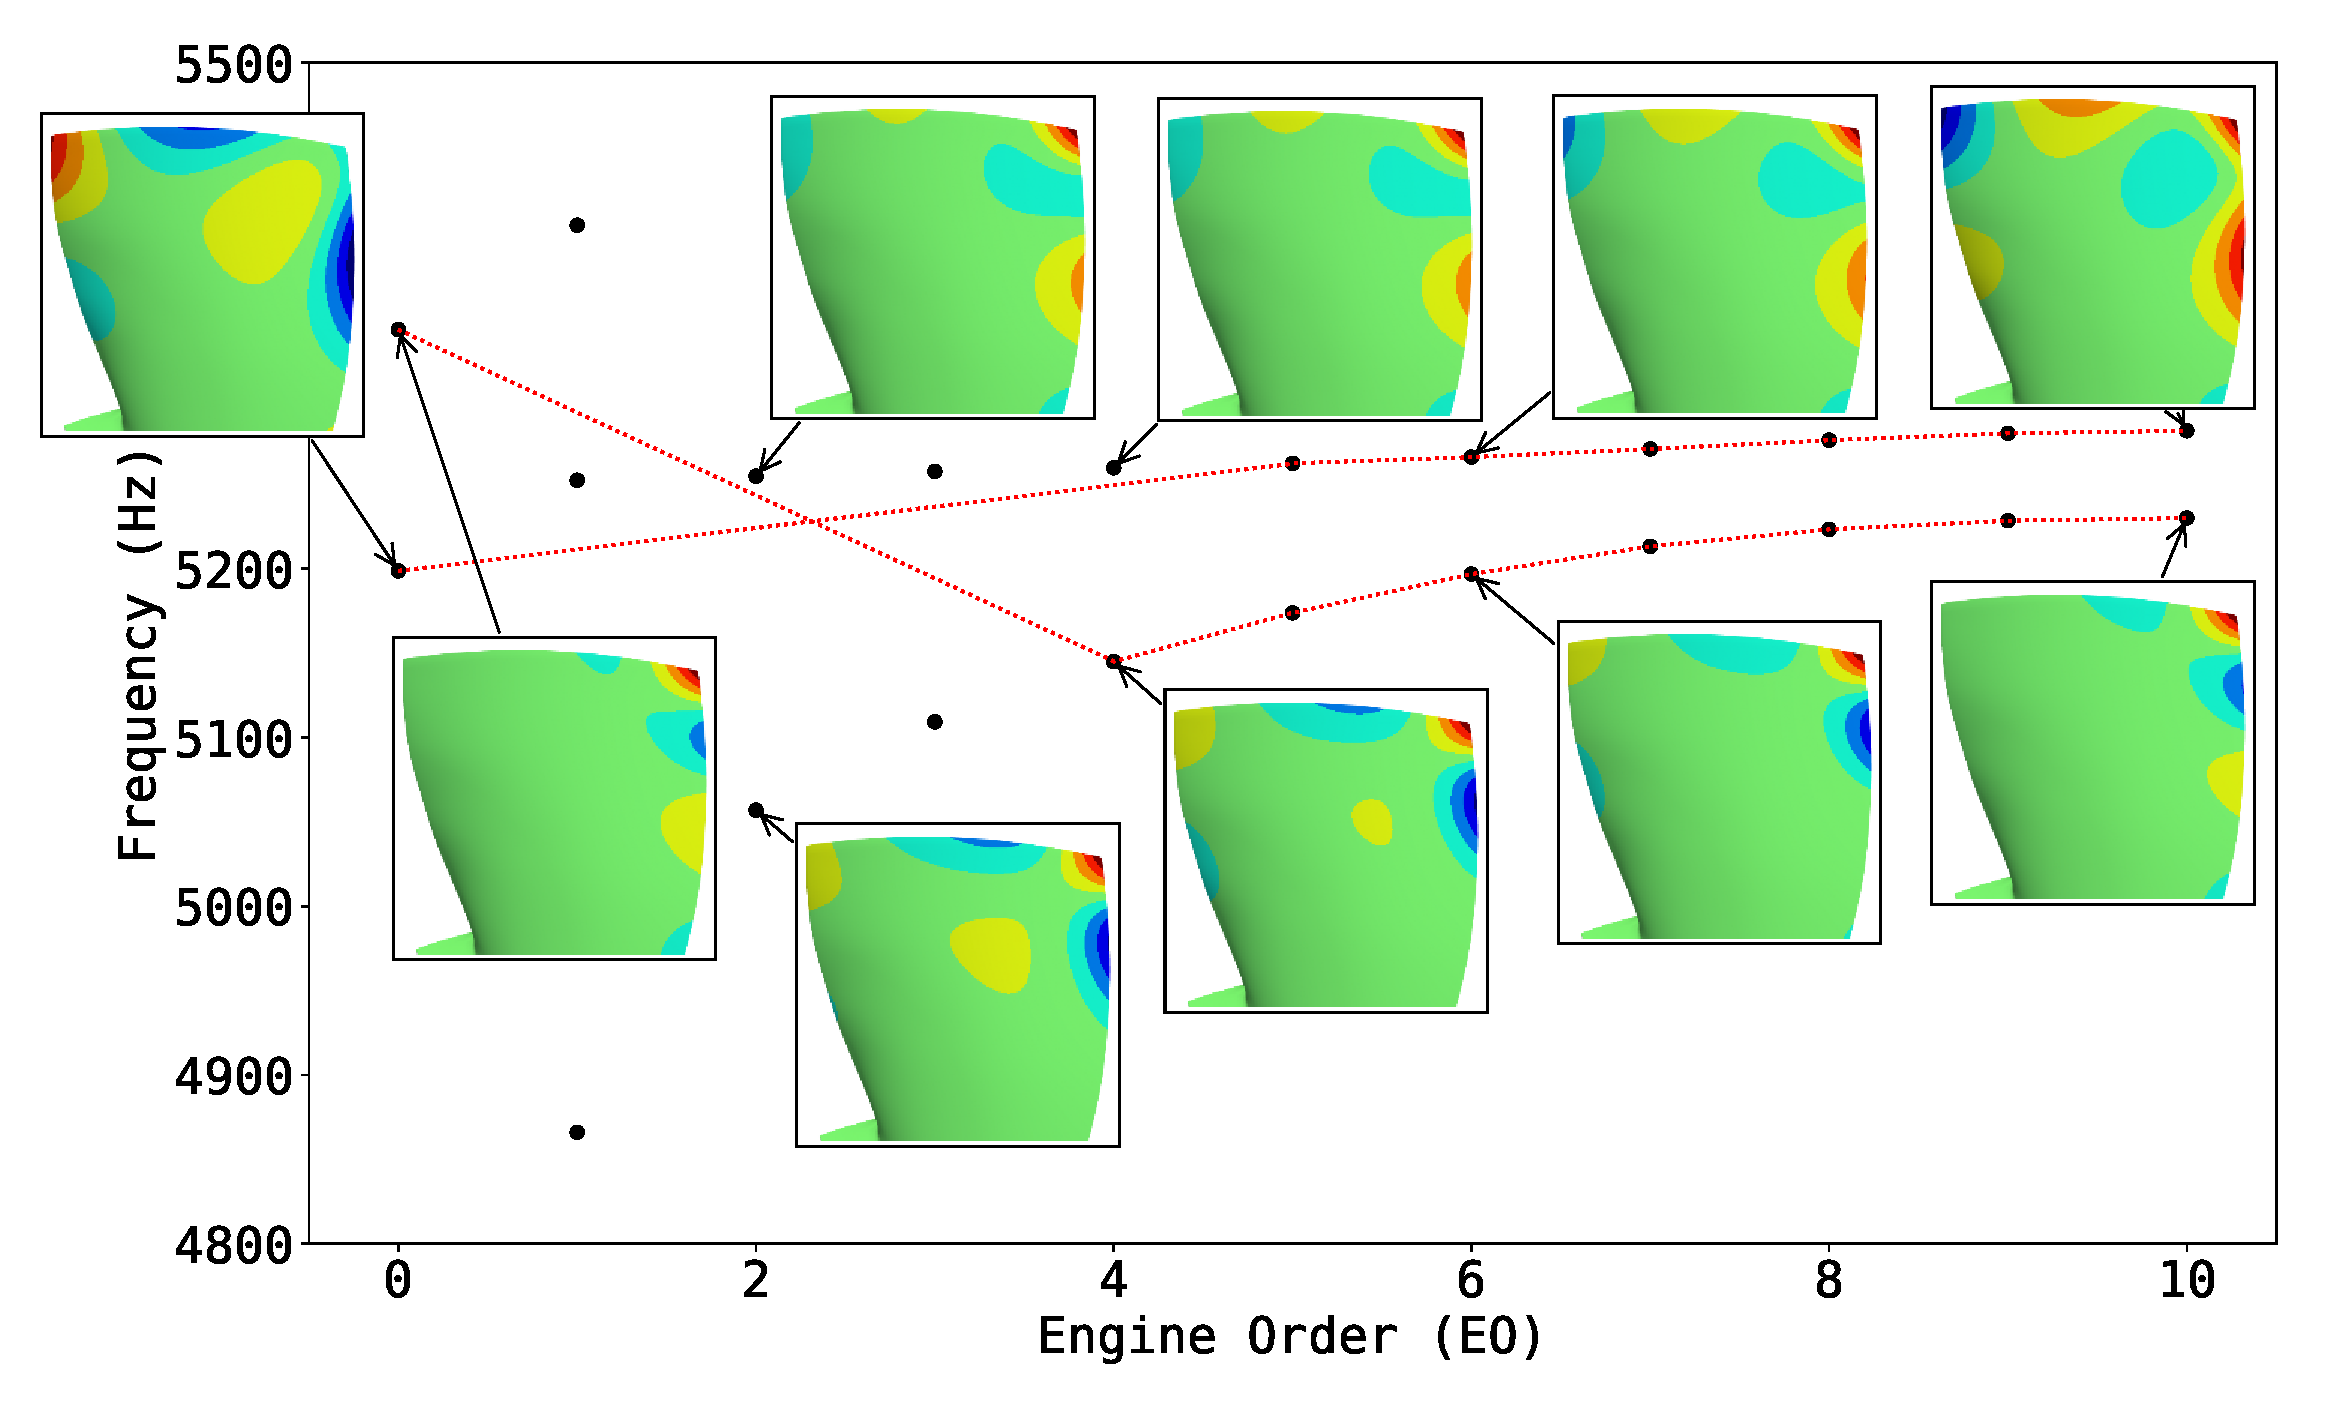
\includegraphics[width=\linewidth, alt = {GMM Modes 9 and 10 - Nodal Diameter Plot}]{figures/tuned-comparison/Figure14.eps}
    \caption{GMM nodal diameter plot -- modes 9 and 10 }
    \label{fig:nd-mode-9-10}
\end{figure}

The mode swapping between modes 9 and 10 appears to be driven both by the frequency proximity of the two mode families and their disk participation as highlighted by the annotated nodal diameter plot in Figure \ref{fig:nd-mode-9-10}. The figure highlights how the lower EO mode shapes appear to ``swap'' compared to their higher engine order counterparts. While the swap is imperfect, the red dotted line highlights how EO 0 maintains a MAC of $0.7$ with the swapped mode. While this behavior alone is insufficient to predict mode swapping in the isolated blade mode shapes, it does appear to strongly indicate that the natural frequency of the mode influences its mode shape. The GMM and isolated blade-alone sector mistuning deviations vary by as much as $\pm 3\%$, or approximately between 4,850 - 5,150 Hz, well within the tuned overlap region of the two modes shown in Figure \ref{fig:nd-mode-9-10}, and indicating mode swapping should be observed in the experiment and predicted in the GMM.

\begin{figure}
    \centering
    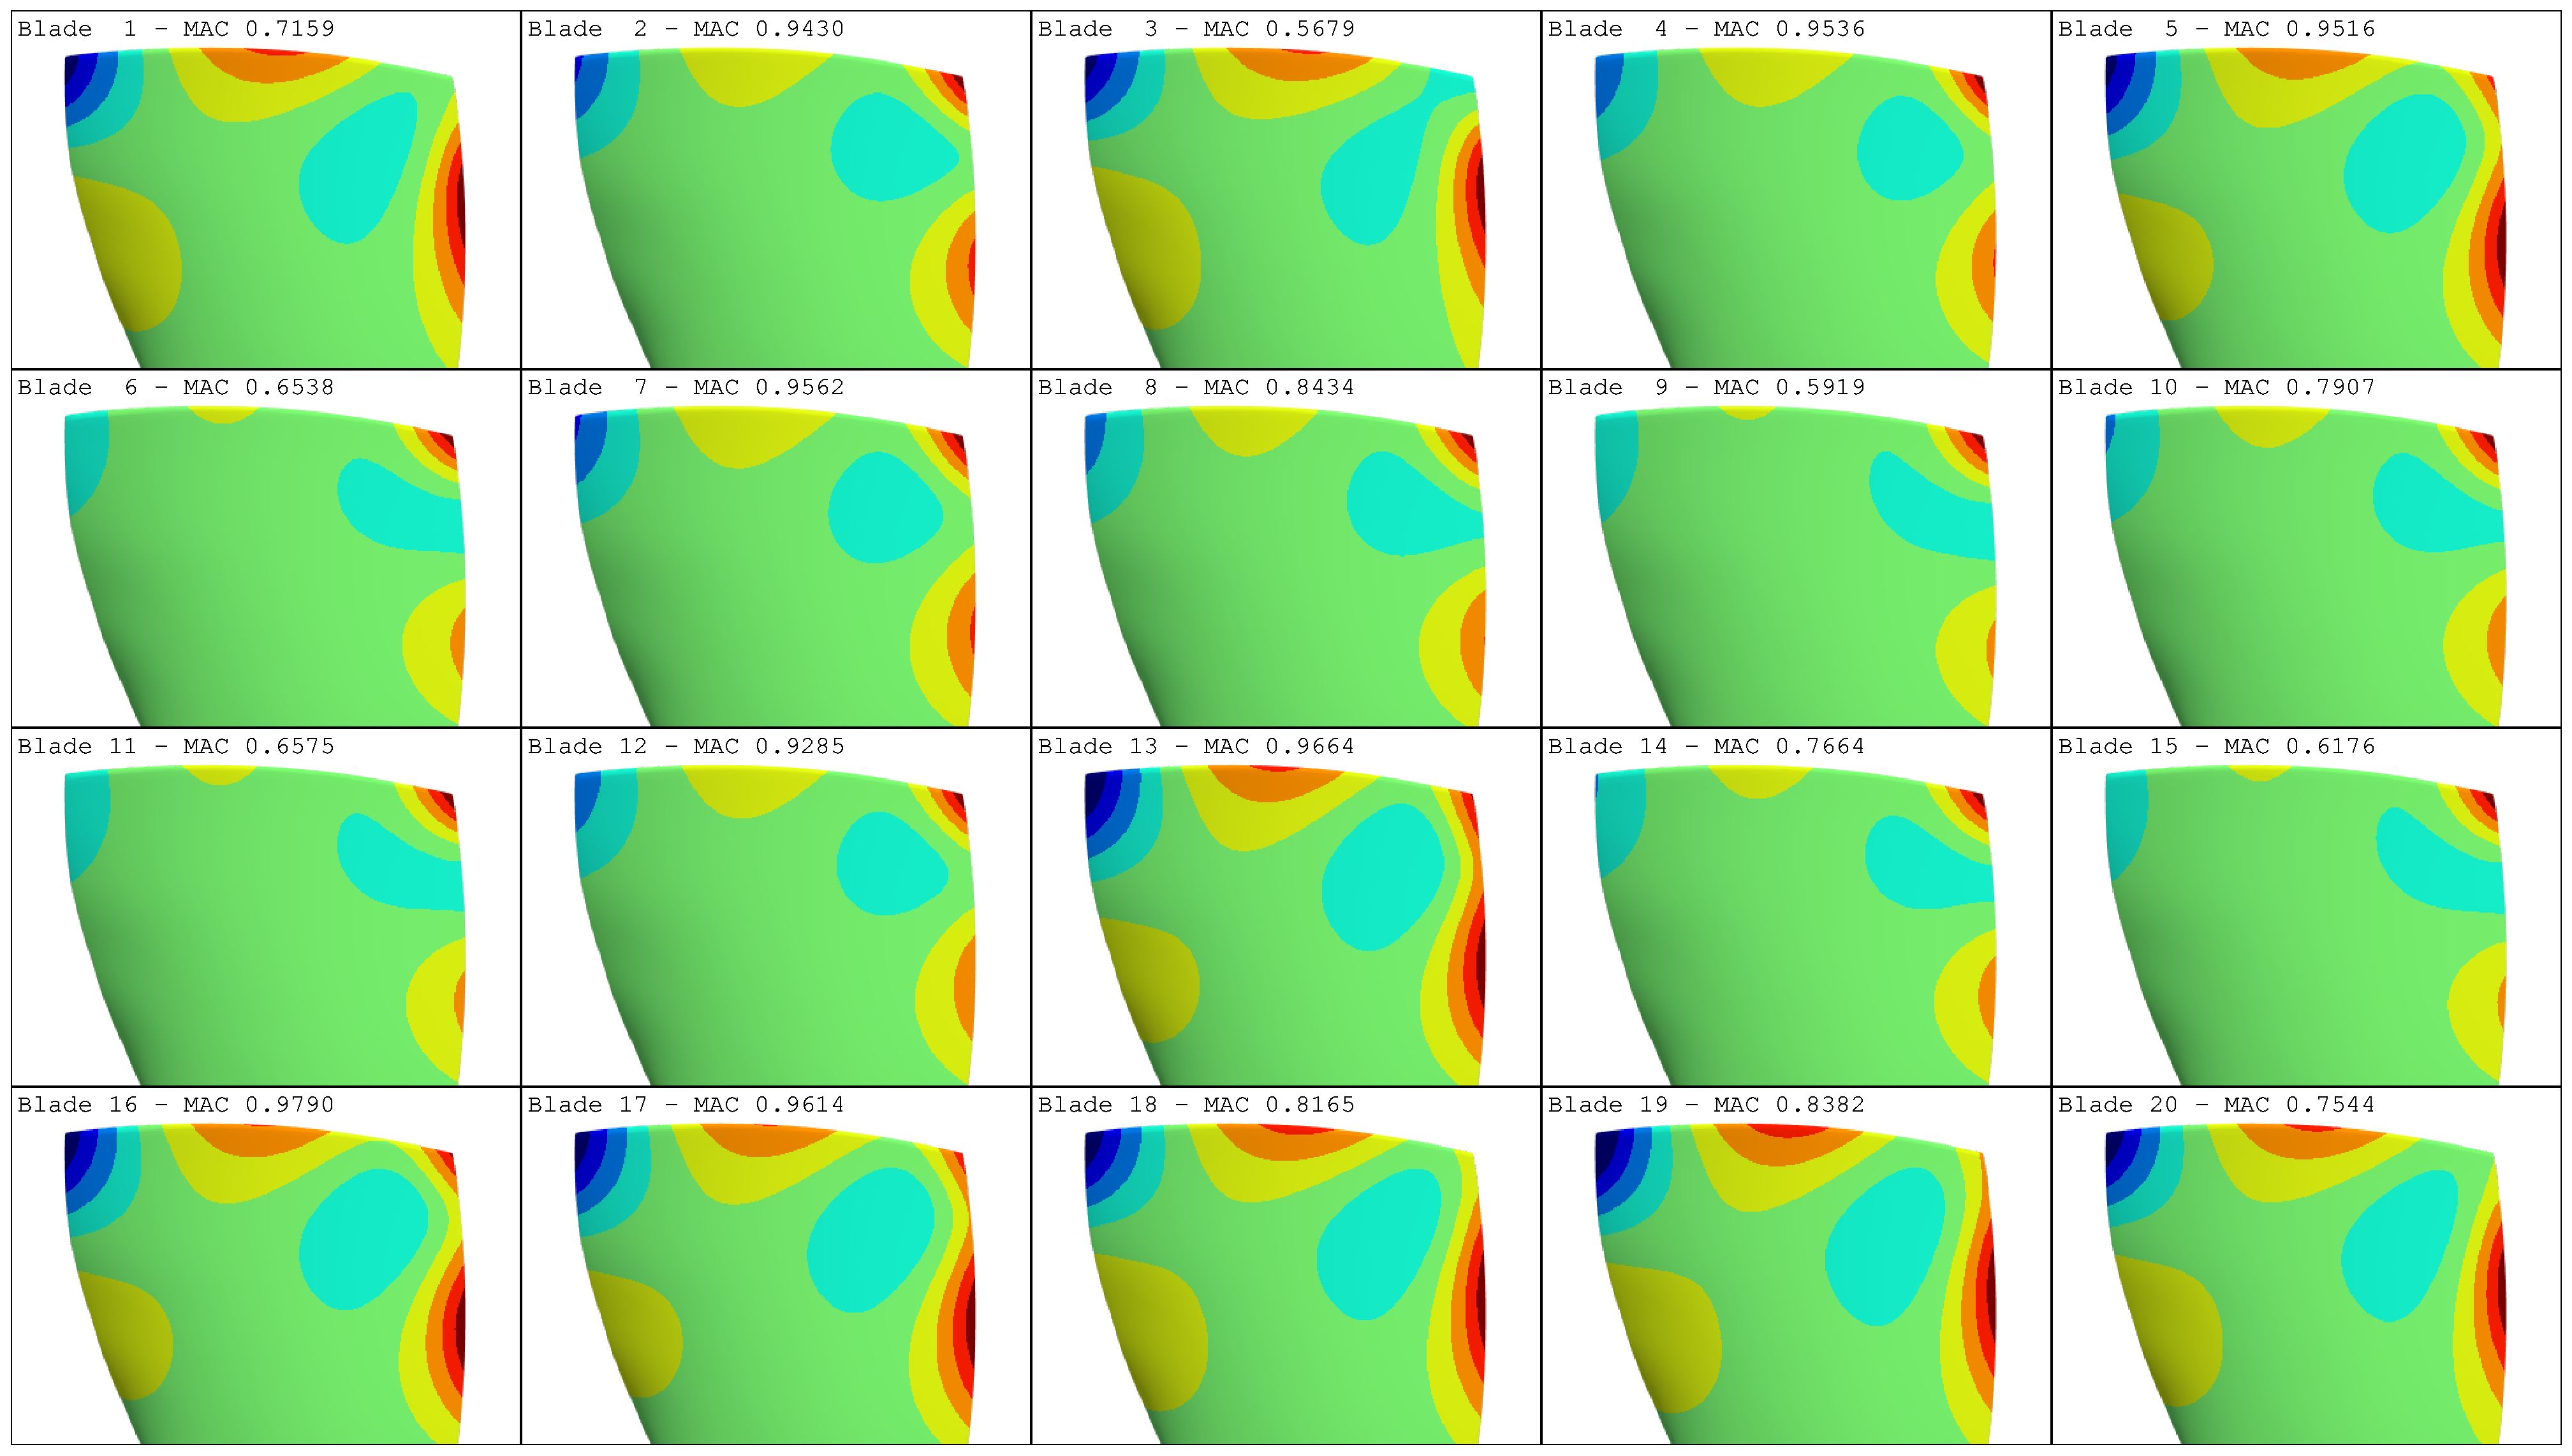
\includegraphics[width=\linewidth, alt = {Mode 10 - GMM Blade Mode Shape Variation}]{figures/mode-10-gmm-exp/Figure15.eps}
    \caption{GMM blade mode shape variation -- mode 10}
    \label{fig:gmm-mode-10}
\end{figure}

\begin{figure}
    \centering
    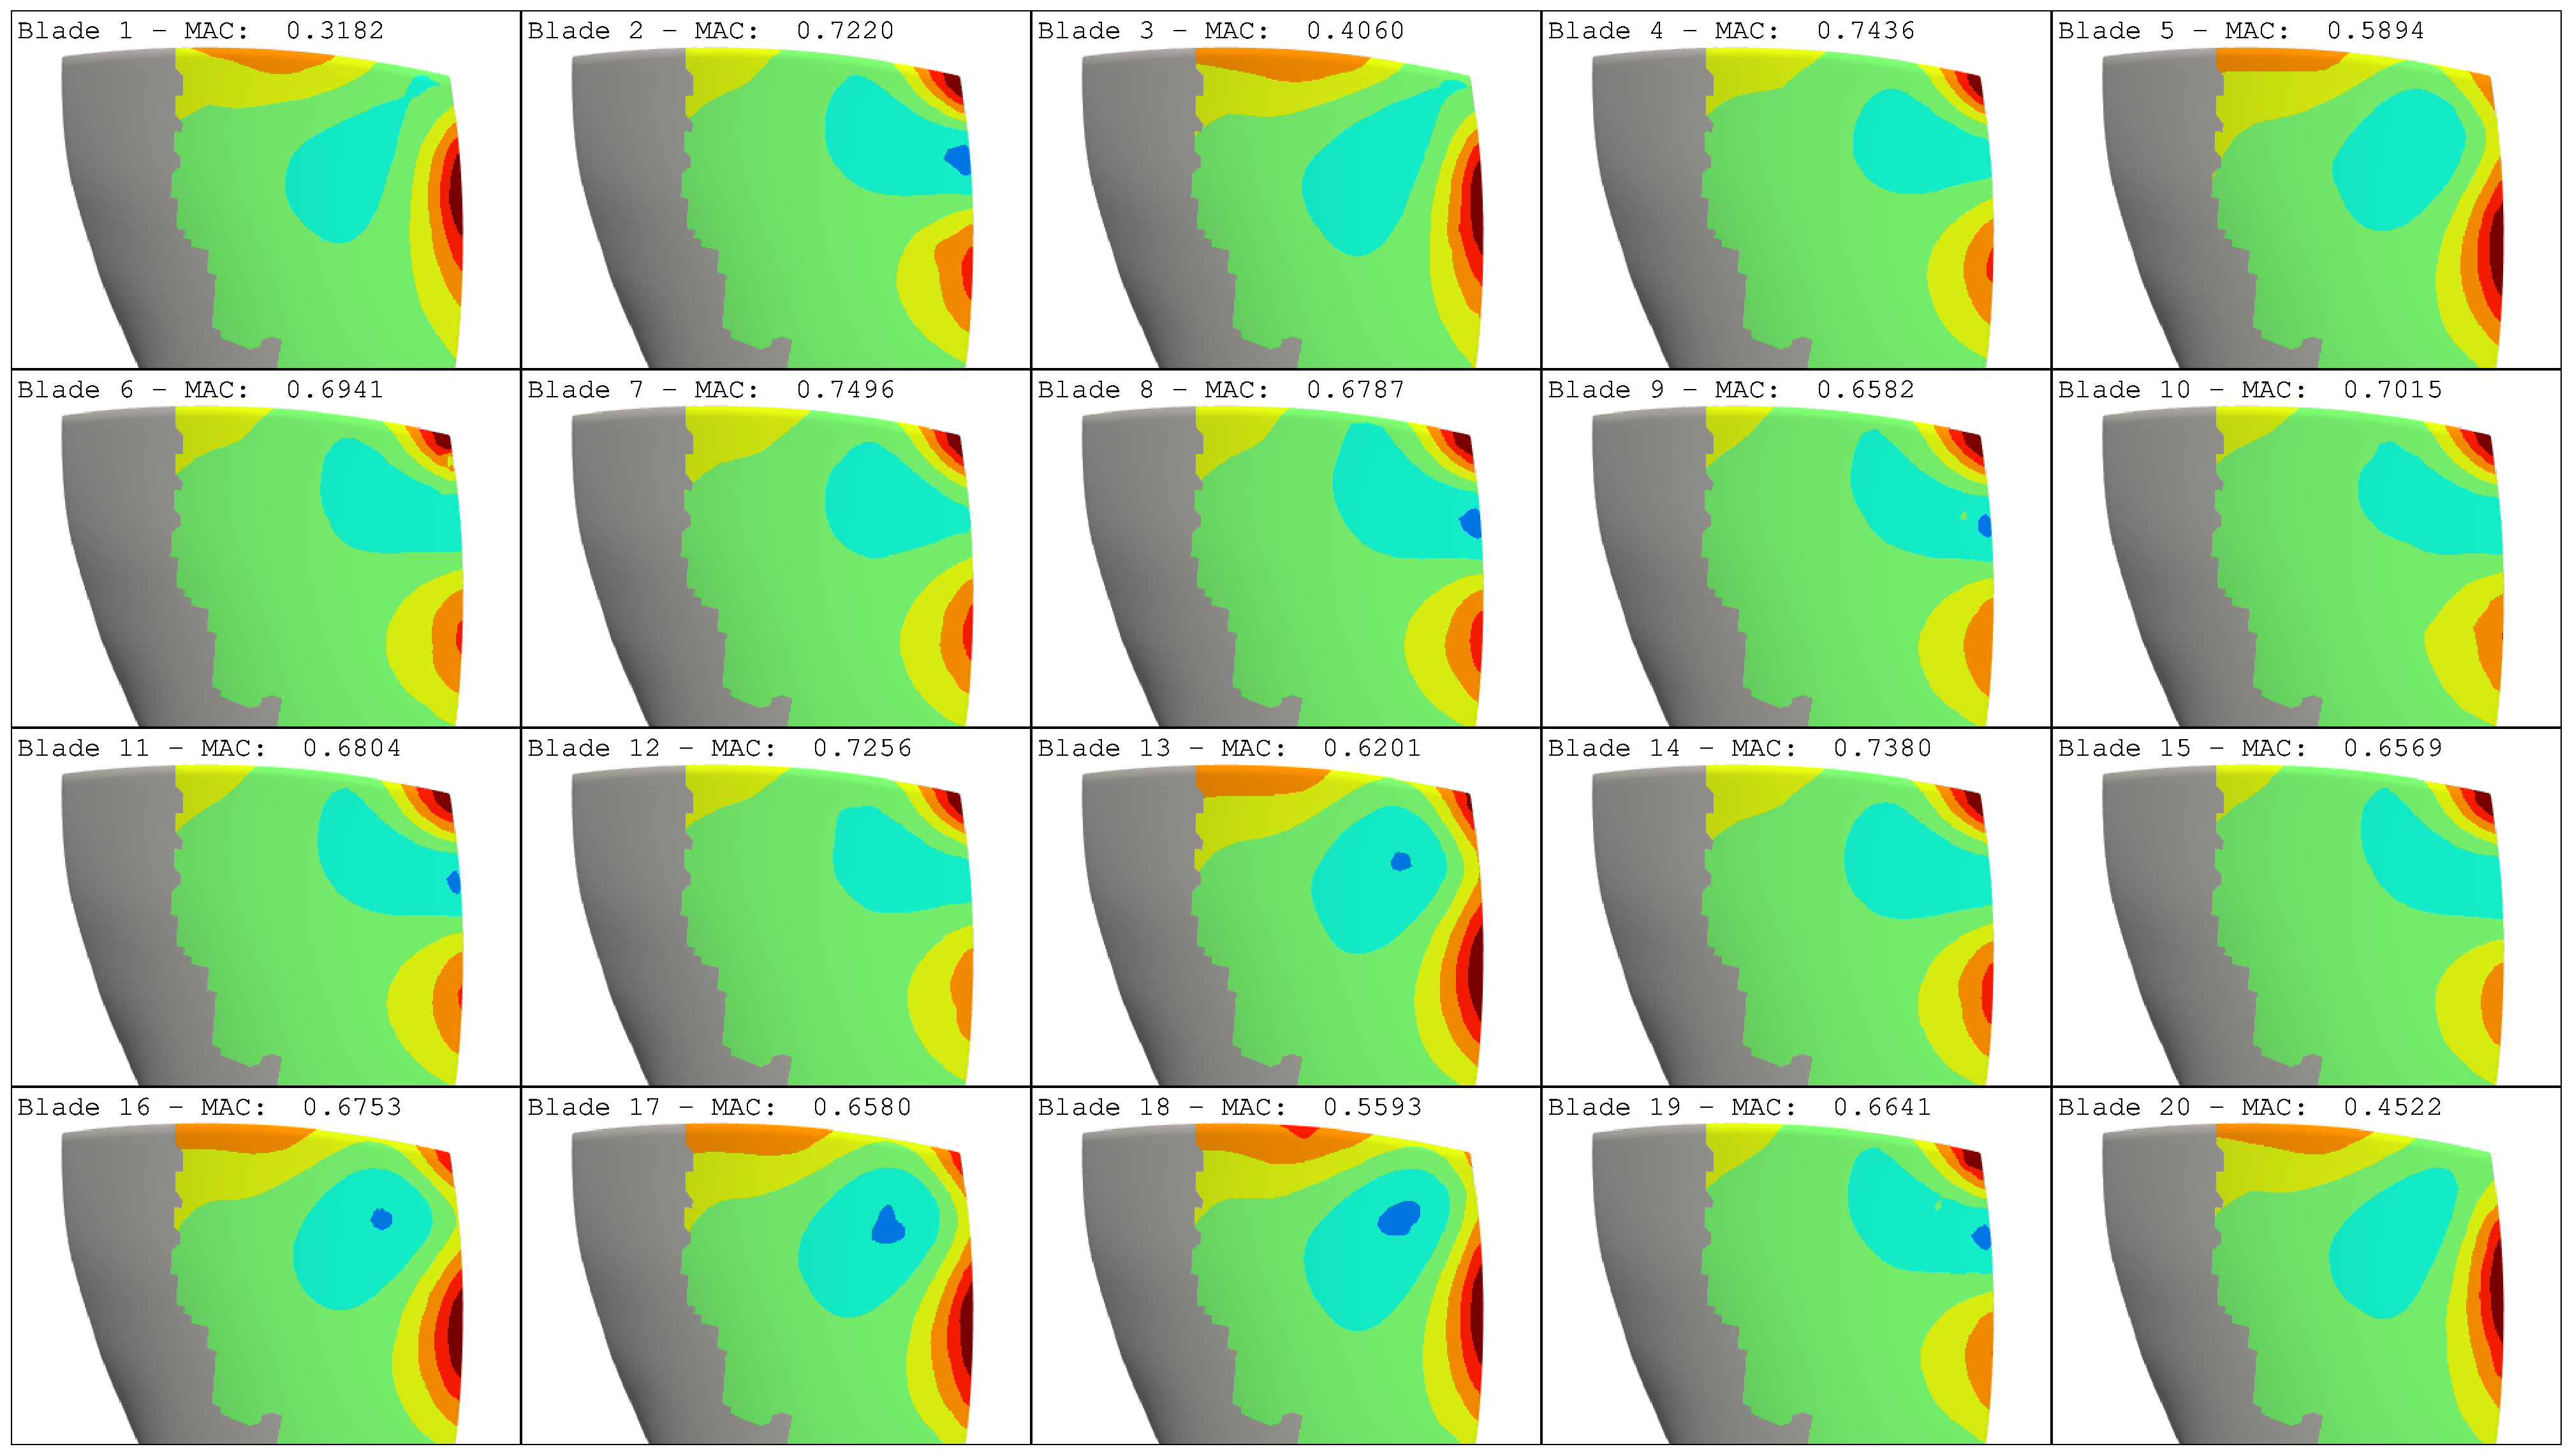
\includegraphics[width=\linewidth, alt = {Mode 10 - Experimental Blade Mode Shape Variation}]{figures/mode-10-gmm-exp/Figure16.eps}
    \caption{Mode 10 - experimental blade mode shape variation}
    \label{fig:exp-mode-10}
\end{figure}

Figures \ref{fig:gmm-mode-10} and \ref{fig:exp-mode-10} show the mode shapes for Mode 10, the mode from Table \ref{tab:iso-exp-table} with the highest value of  $\overline{\mathrm{MAC}}_{i<j}$ ($0.5737$), and therefore, the largest inter-blade mode shape variation among all observed modes. The MACs shown in the figure are between the tuned mode and the observed isolated blade mode. Despite the large mode shape variation, the GMM strongly agrees with the isolated blade mode shapes, as shown by the aforementioned figures, and also from the high diagonal MAC score between the GMM and isolated experimental results of $0.9026$. The mean diagonal blade MAC score $\overline{\mathrm{MAC}}_{i=j}$ is calculated by

\begin{equation}\label{eq:mac_diag}
    \overline{\mathrm{MAC}}_{i=j} = \frac{1}{N} \sum_{i=1}^{N} \mathrm{MAC}_{ii}
\end{equation}

\noindent
and is the mean of the MAC scores between GMM blade $i$ and experimental blade $i$ for a single mode. The value of $0.9026$ indicates that the GMM can accurately predict the mode shape of nearly all the blades despite the variation due mode swapping. The GMM failed to achieve a MAC of at least $0.83$ to the experimental blade mode shapes for only a single blade, blade 19, with a poor MAC agreement of $0.1226$ to mode 10 and also a MAC score $0.4607$ for mode 9, showing how mode swapping affects mode pairs, not just isolated modes.

There were several attempts to fully capture the mode swapping behavior for the 19\textsuperscript{th} blade. Each GMM constructed from each geometry dataset was compared to the experimental results, and the last two GMMs from the final two scans achieved the highest MAC score with the experiment, with the initial four showing excellent agreements as well, except for the mode swap pair (9 and 10). The number of reference points used on the scans was increased throughout the scanning process, with the final two scans having the highest number of reference points concentrated near the blade tips. The minor reduction in reference point deviation and improved scan accuracy improves the accuracy of the GMM and the mode swap pair. However, even with the more accurate GMM, the 19\textsuperscript{th} blade's mode shape still did not match the experimental results. Increasing the density of the FEM also did not improve the correlation within this frequency range: there was almost no difference when increasing the density of the sector model for this mode. The mode shapes from the denser GMM obtained a $\overline{\mathrm{MAC}}_{i=j}$ of $0.8886$ for mode 9 and $0.8994$ for mode 10, a slight improvement for the first and a slight reduction for the second mode.

\begin{figure}
    \centering
    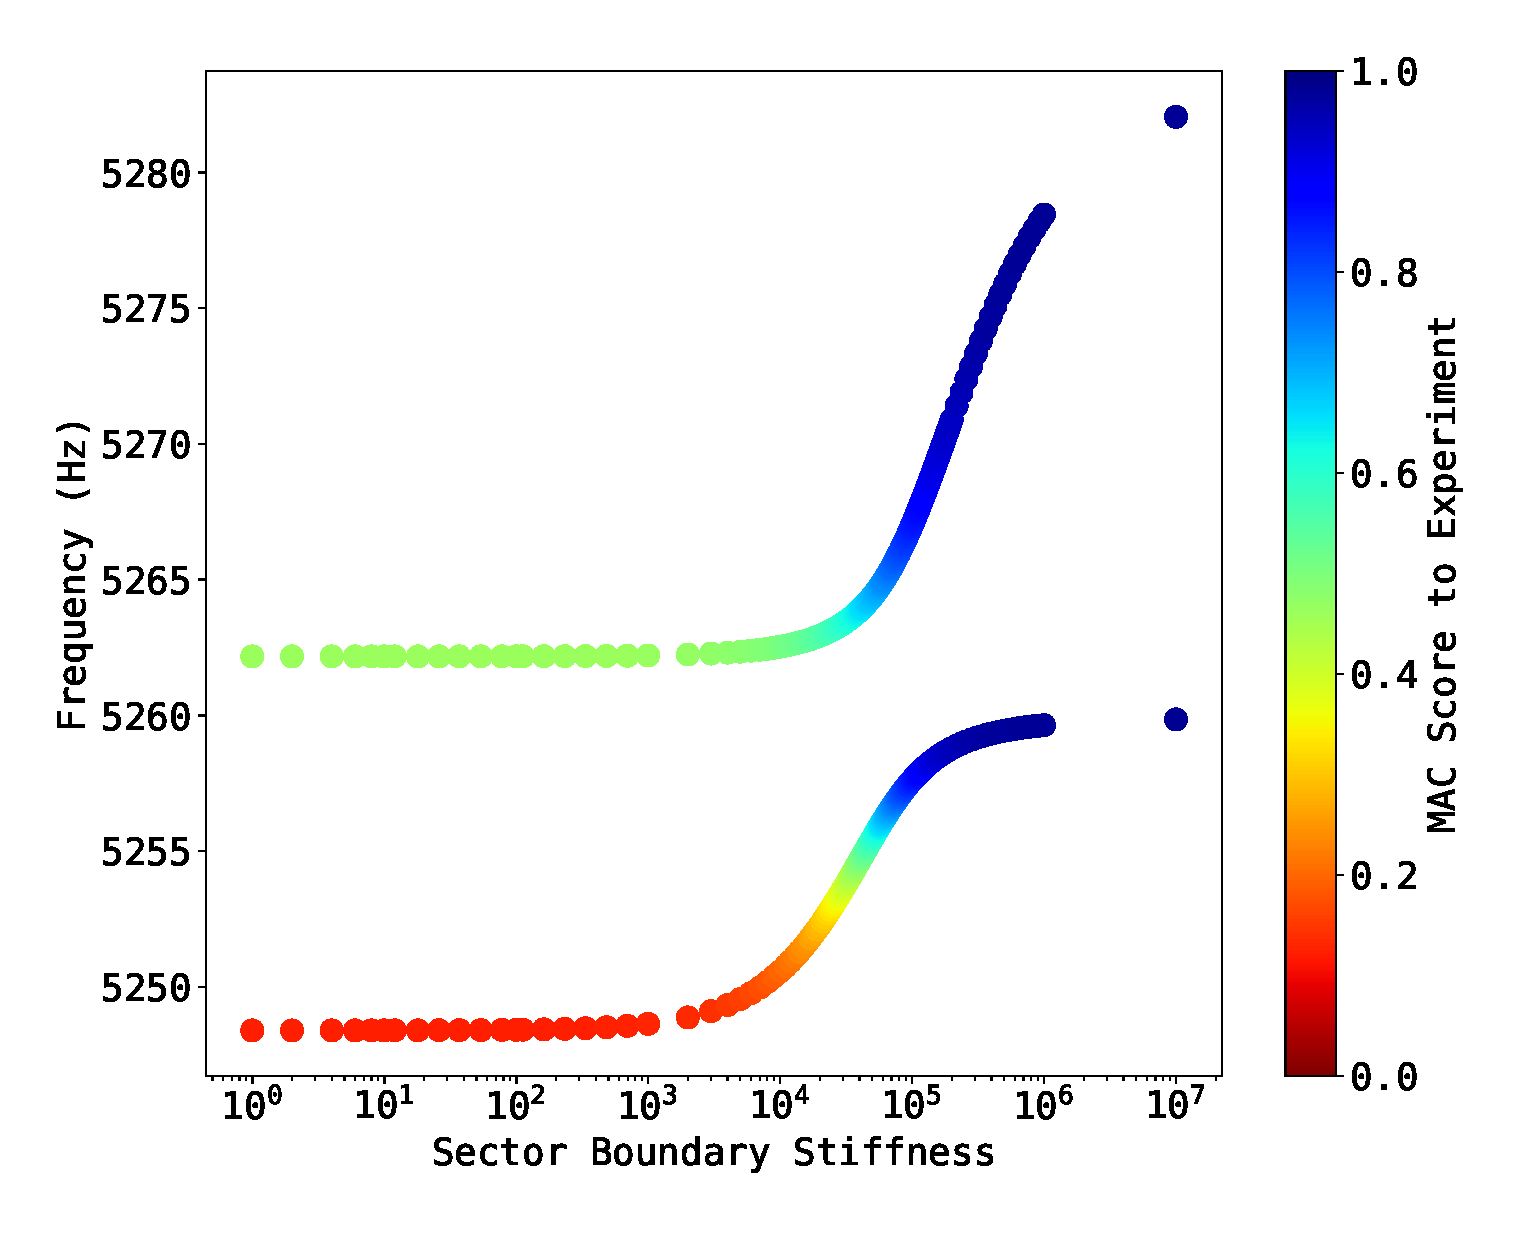
\includegraphics[width=\linewidth, alt = {Blade 19 Mode Swapping due to Sector Stiffness}]{figures/mode-swapping-stiffness-blade-19/Figure17.eps}
    \caption{Blade 19 -- mode swapping due to sector stiffness}
    \label{fig:mode-swapping-blade-19}
\end{figure}

One final attempt was made to modify the GMM to obtain better agreement for blade 19 based on the assumption that the free-free high EO cyclic analysis did not fully capture the clamping boundary condition. Within MAPDL, LINK14 elements were created at the disk boundary interface nodes to fixed nodes at 0.1$^{\circ}$ behind and 0.1$^{\circ}$ ahead of the low and high cyclic sector interfaces respectfully. The stiffness of these linear elements was varied from 1 to $1\times10^{7}$, allowing for the simulation of intermediate boundary conditions between EO 10 and fixed sector interfaces. While increasing the stiffness improved the correlation for blade 19, it decreased the correlation of the majority of the blades between the GMM and the experimental results. However, during this parameter sweep, the researchers discovered that by smoothly increasing the stiffness of the disk and effectively eliminating disk participation altogether for this mode pair, they were able to observe mode swapping for a single pair of modes for a single blade. Figure \ref{fig:mode-swapping-blade-19} shows how artificially stiffening the sector cyclic boundaries for this blade both shifted the natural frequencies of the modes upward and caused mode swapping to occur approximately at a boundary stiffness of $5\times10^{4}$, right at the inflection point for the change in natural frequency for both modes.

Since modifying the boundary condition did not globally increase the correlation to the experiment, it is assumed that the free-free boundary condition is valid and the mode swapping behavior is an artifact of slightly incorrect geometry, either due to post-scanning damage, scan noise, or, unlikely, material property variation for only blade 19. Regardless, it is observed that mode swapping for these closely spaced modes is incredibly sensitive and, at least in part, a function of disk participation.

It should be noted that this mode swapping behavior appears to be driven by the proximity in frequency of the two modes and not disk participation. The largest change in the mode shape for both modes occurred as the two modes were the closest in natural frequency. Also, note that although this mode swapping behavior should not be confused with mode family veering. In mode family veering, decreasing disk participation due to a change in apparent disk stiffness causes the frequency of the mode within a mode family to ``veer'' relative to adjacent mode families. Instead, this specific mode swapping phenomenon appears to be caused by the harmonic proximity of two modes of a single isolated blade. The researches have discovered that by artificially stiffening the sector boundary in the GMM, the mode pair can be made to undergo mode swapping, allowing the direct observation of the phenomenon in a single mode pair for a single blade.

\subsection{Mode Swapping in the Full Rotor}

The prediction and observation of mode swapping for the 5~kHz mode pair has significant implications, especially if the mode swapping also occurs within the full mistuned rotor. First, any instrumentation used for OMA or stress monitoring of the rotor cannot assume consistent mode shapes between blades of the rotor, as first identified by Gillaugh et al.\ \cite{Gillaugh2018, Gillaugh2019}. Nor can OMA be used for mode identification based on frequency alone as, at least according to the isolated blade analysis and experimental results, blade mode shapes vary even within mode families. The assumption that this behavior occurs in the full rotor GMM and experiment will be demonstrated.

\begin{figure}
    \centering
    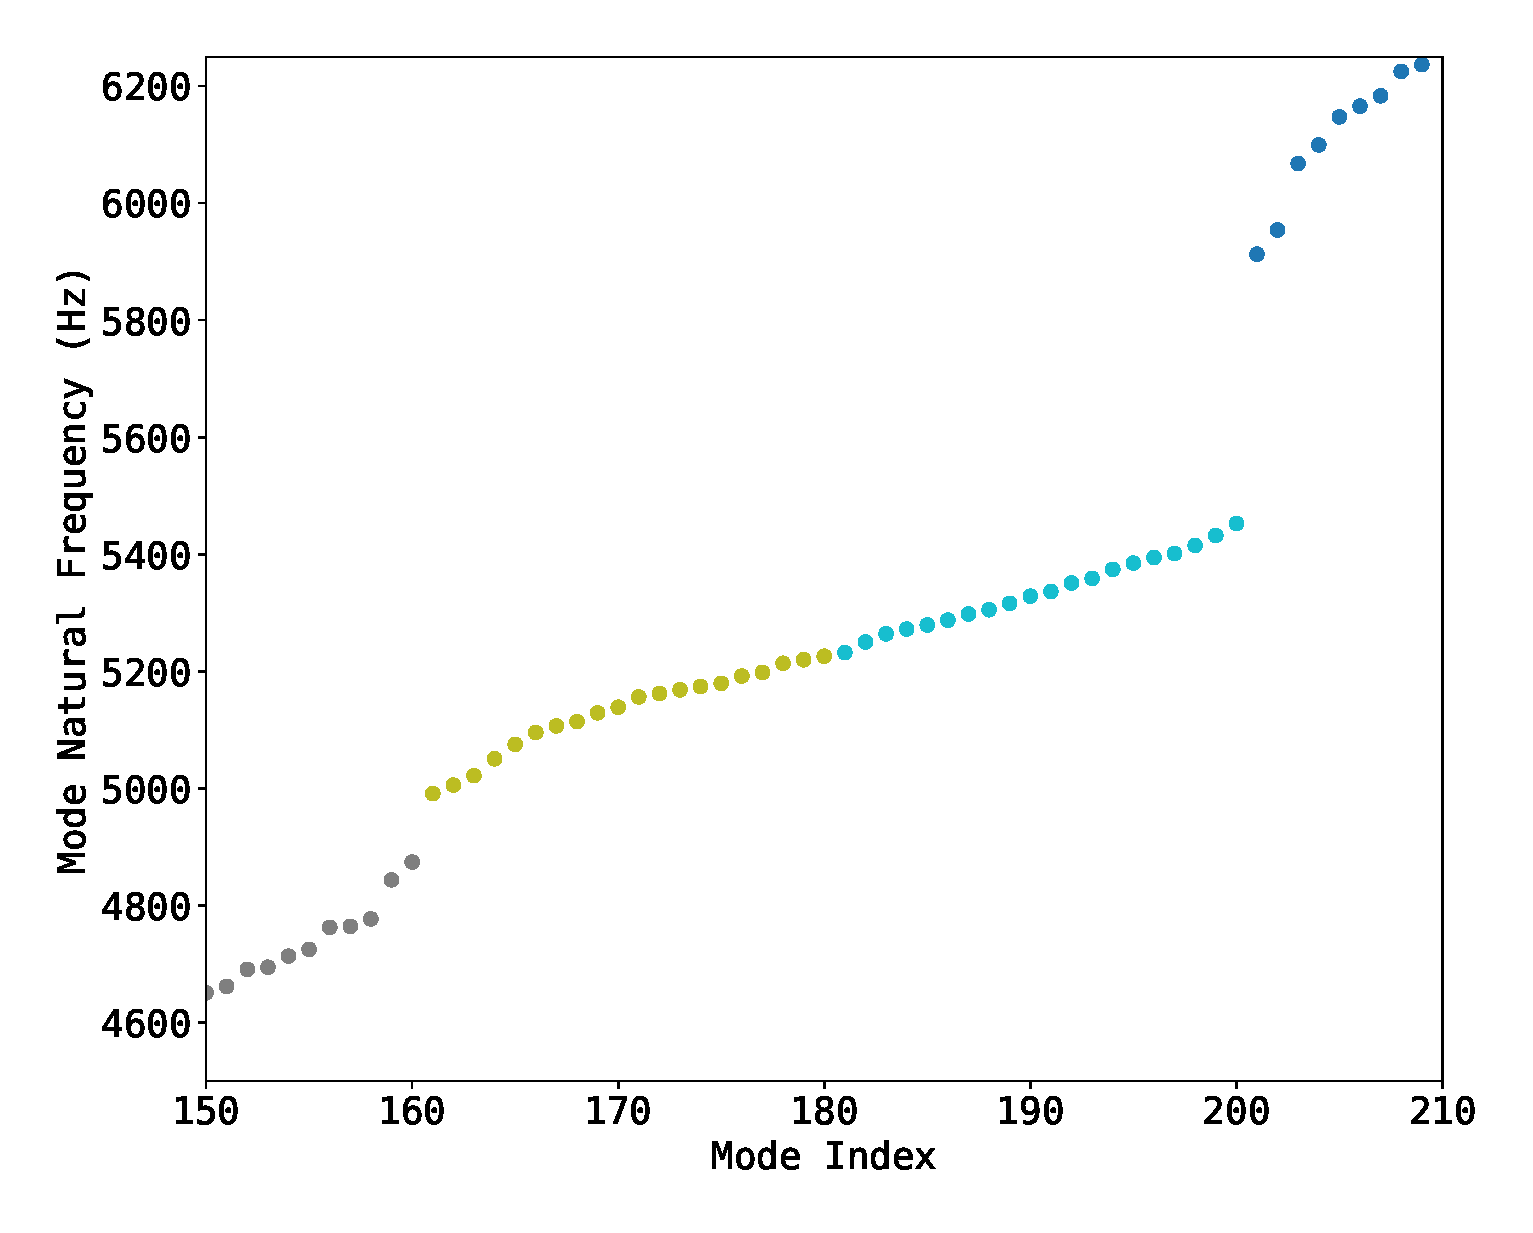
\includegraphics[width=\linewidth, alt = {Full Rotor Mode Swap Pair Groups}]{figures/full-rotor/Figure18.eps}
    \caption{Full rotor modes -- The two mode swap families are shown grouped between 5~kHz and 5.4~kHz}
    \label{fig:full-rotor-swap-pair-wn}
\end{figure}

To confirm this behavior analytically, a free-free modal analysis of the full mistuned rotor GMM (2,279,880 nodes) was performed within the frequency range of 0.5~Hz to 10~kHz, and the first 400 full rotor modes were collected. Figure \ref{fig:full-rotor-swap-pair-wn} colors the natural frequencies of the modes by groups of 20, and the two middle groups representing modes 161 to 200 are clearly separate from their adjacent neighboring mode families while showing no separation between the two ``swap'' mode families. Typical tuned full rotor mode families might display this behavior for close, even overlapping modes, but each full mode would only be expected to contain a single mode shape. Instead, due to isolated blade mode swapping it is expected that the modes of the full mistuned rotor would express a combination of the swapped modes simultaneously.

\begin{figure}[bp]
    \centering
    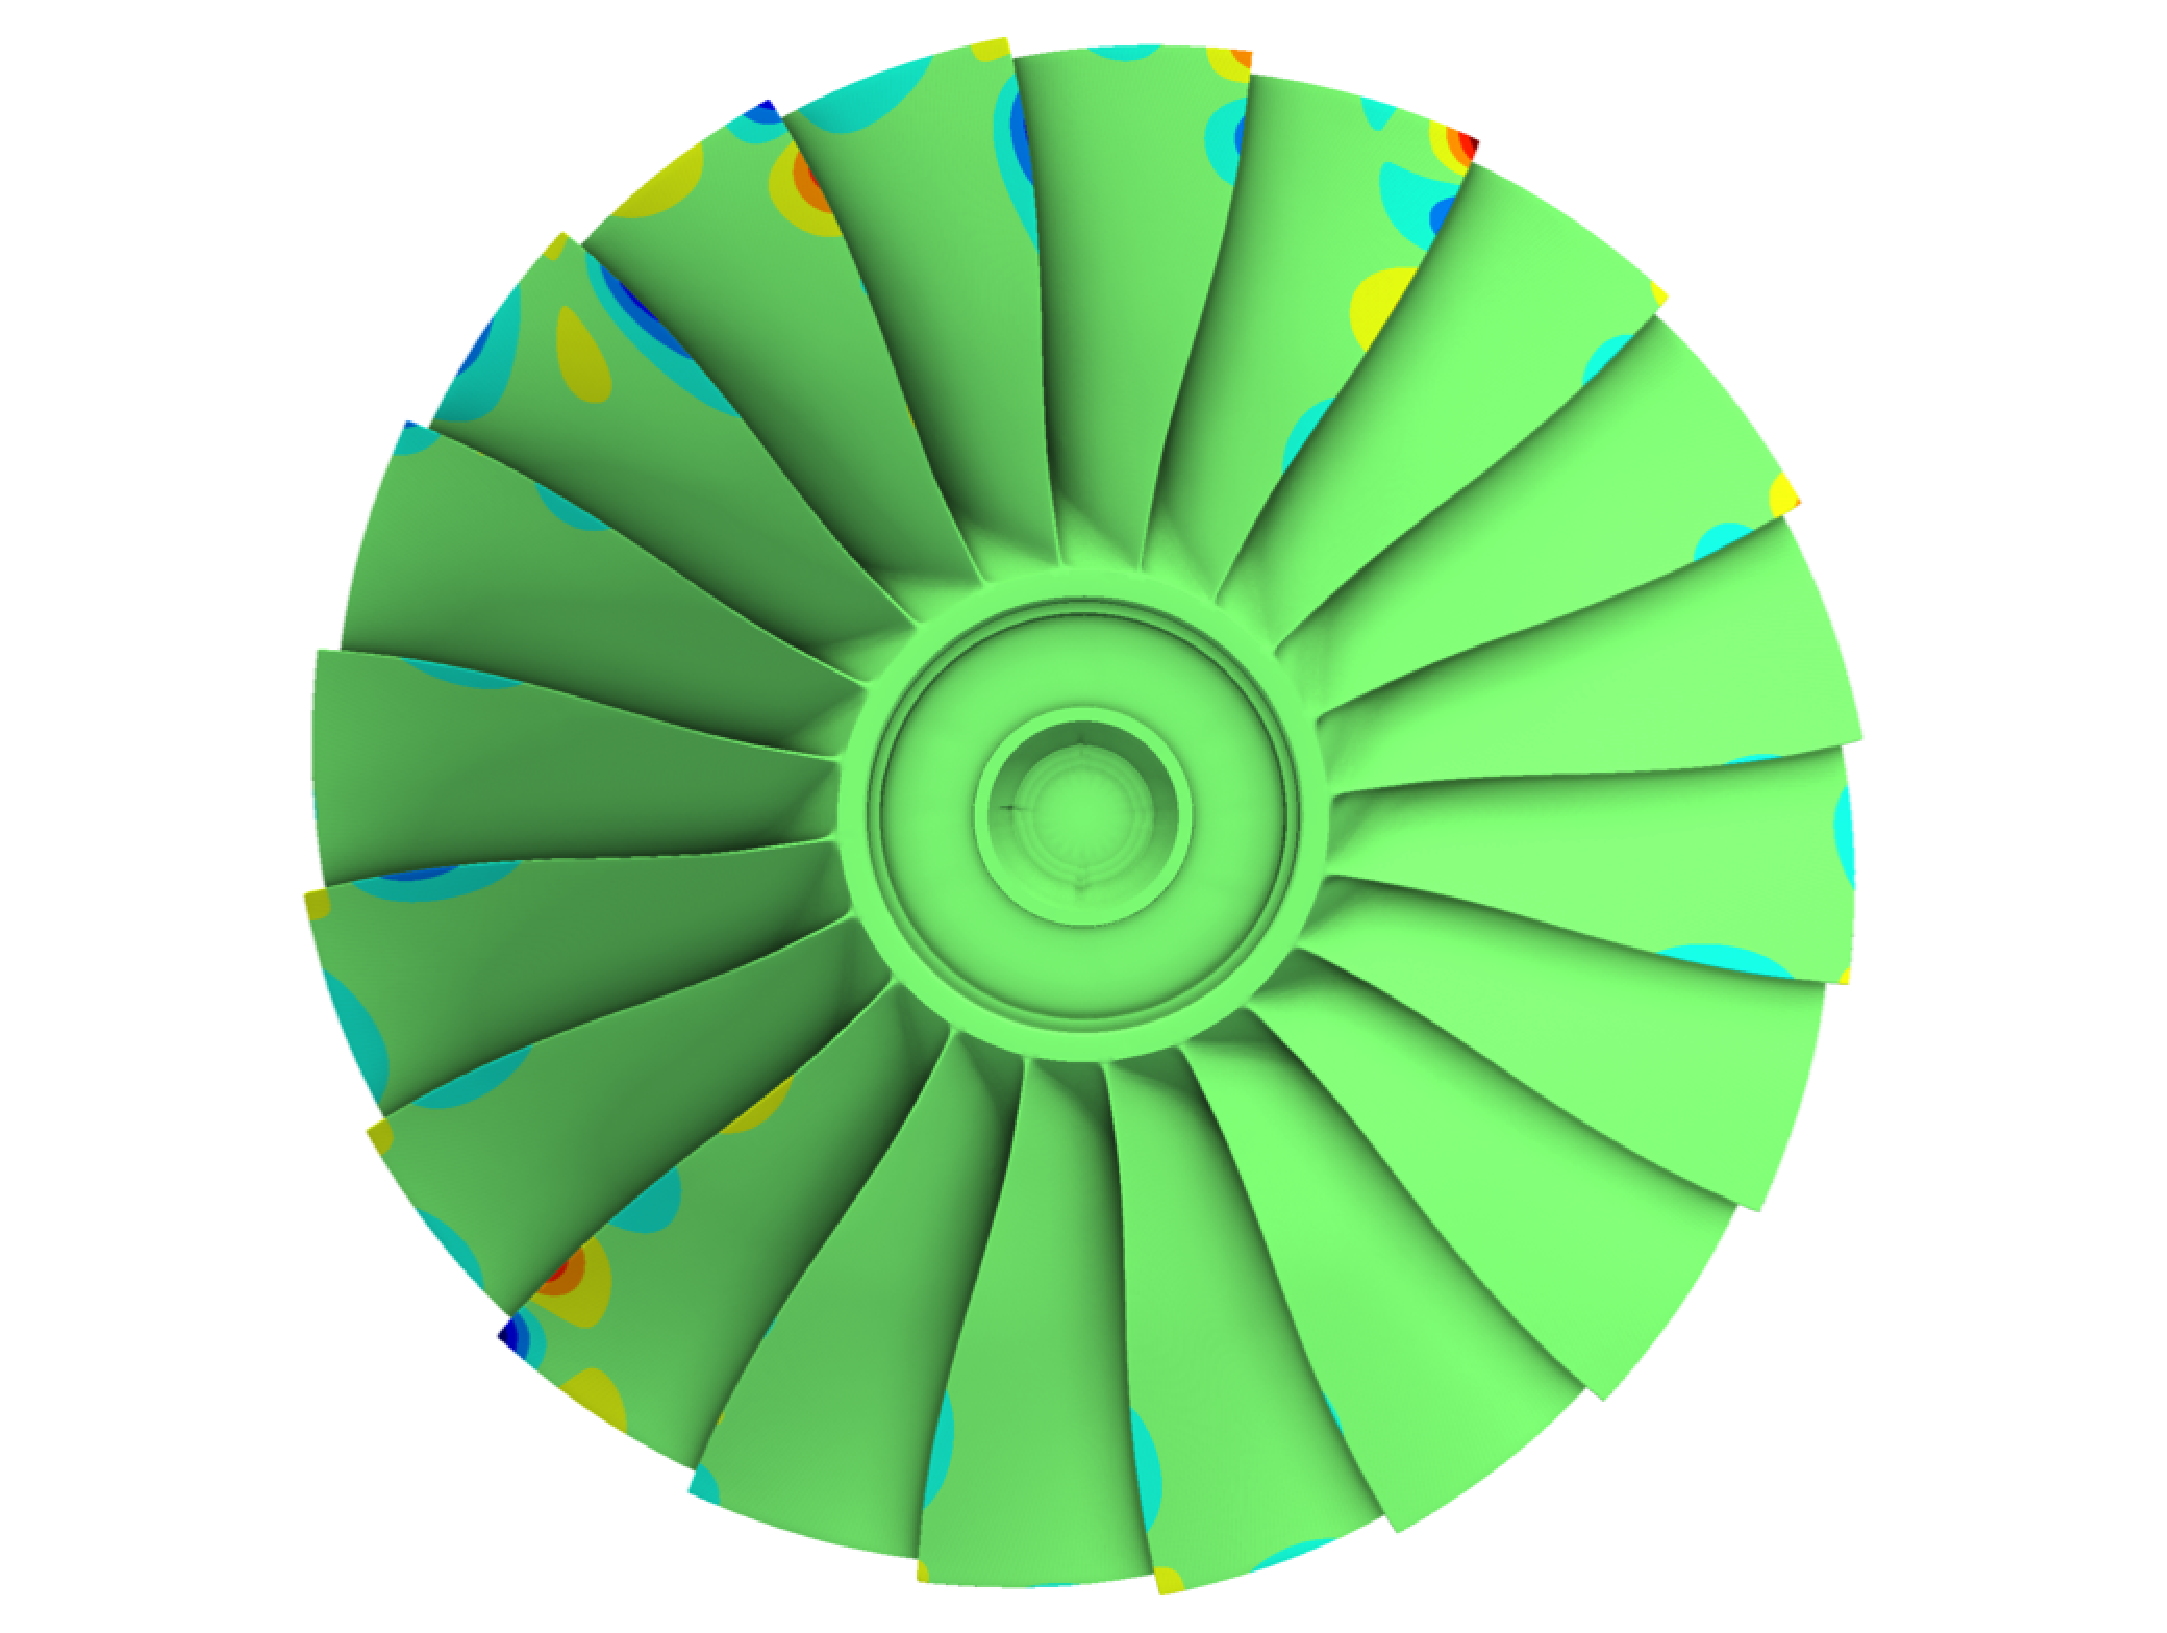
\includegraphics[width=0.5\linewidth, trim=140 0 120 0, clip]{figures/full-rotor/Figure19a.eps}%
    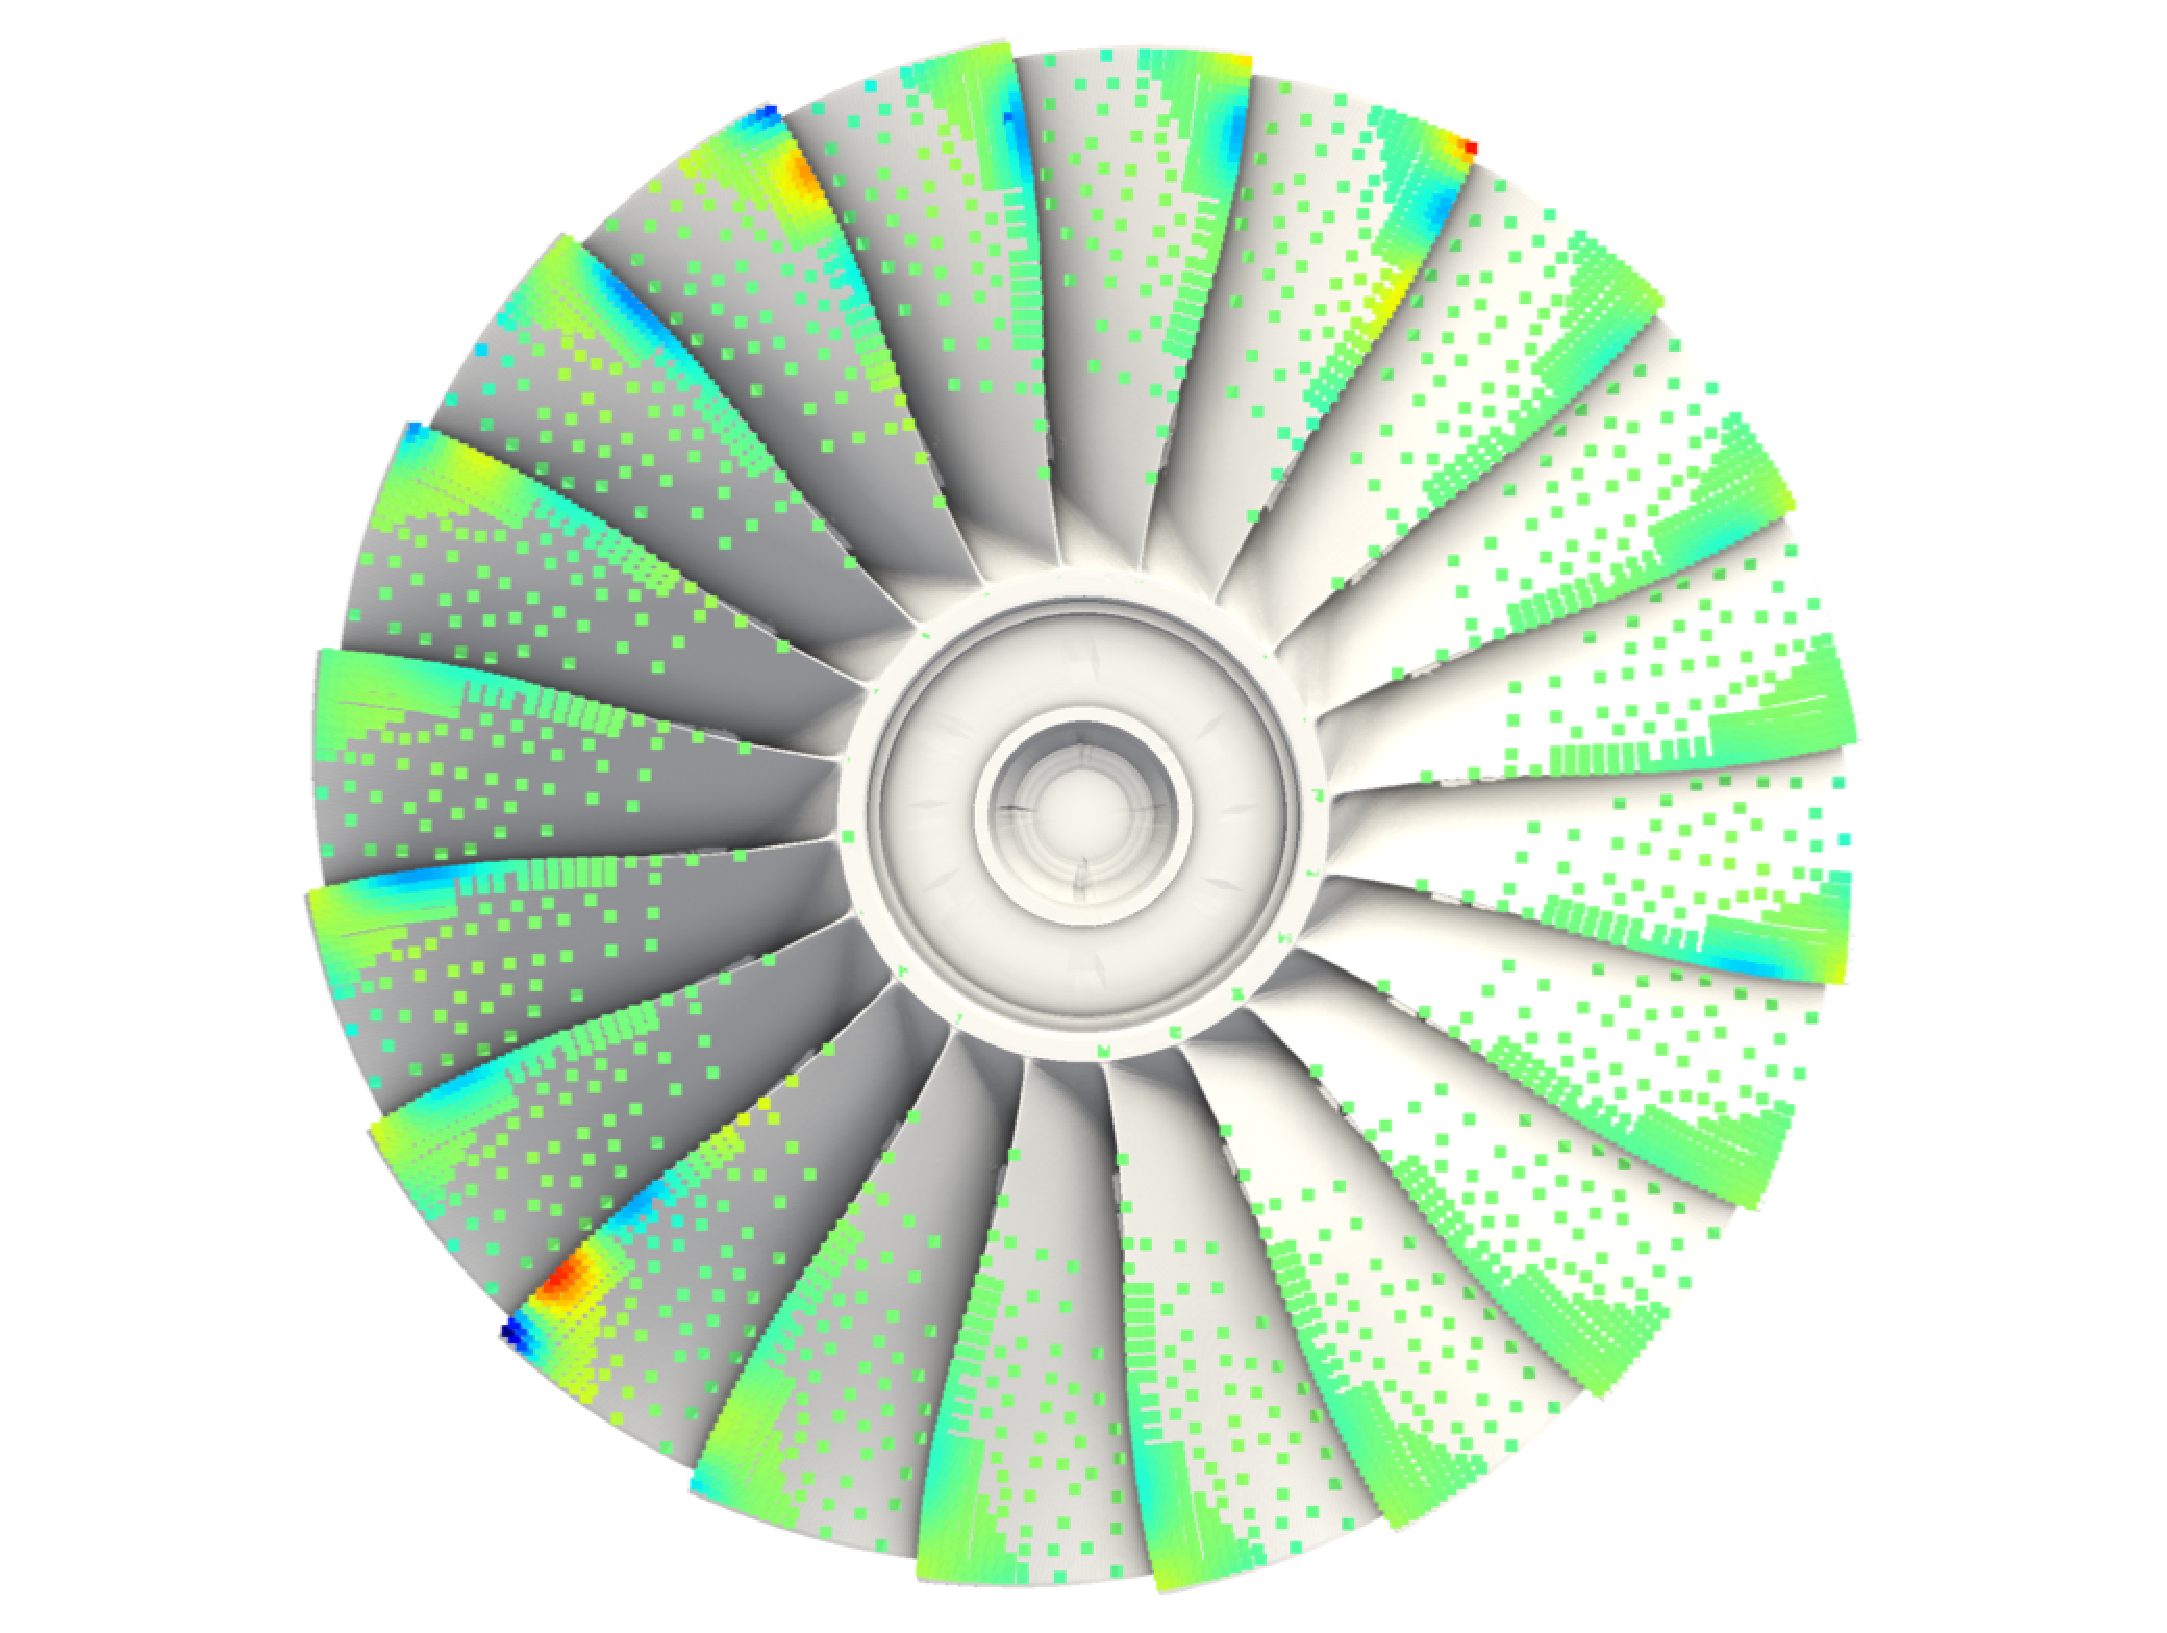
\includegraphics[width=0.5\linewidth, trim=120 0 140 0, clip]{figures/full-rotor/Figure19b.eps}
    \caption{Full rotor mode 176 -- GMM prediction (left) vs. mode from TWE (right)}
    \label{fig:full-rotor-mode-176-comparison}
\end{figure}

Nearly all of the full modes from the two families (modes 161 to 200) exhibit some degree of mode swapping. Mode 176 at $5191.91$ Hz exhibits both this behavior and the modal energy confinement expected from a mistuned mode and is shown on the left of Figure \ref{fig:full-rotor-mode-176-comparison}. This mode was chosen for its relatively low mistuning amplification and to show both mode families 9 and 10 simultaneously in a single full mistuned mode. This behavior also occurs for modes with high mistuning amplification, such as mode 192 at $5350.97$ Hz and shown on the left of Figure \ref{fig:full-rotor-mode-192-comparison}, where the majority of the energy is concentrated within blades 8, 9, and 10 (with blade 1 starting at the 12 o'clock position). Given the ability of the GMM to accurately predict the isolated blade mode shapes and full rotor sector mistuning deviations, it is expected that these predicted mode shapes will be observed in the full experimental response (shown in the right of Figures \ref{fig:full-rotor-mode-176-comparison} and \ref{fig:full-rotor-mode-192-comparison}).

\begin{figure}
    \centering
    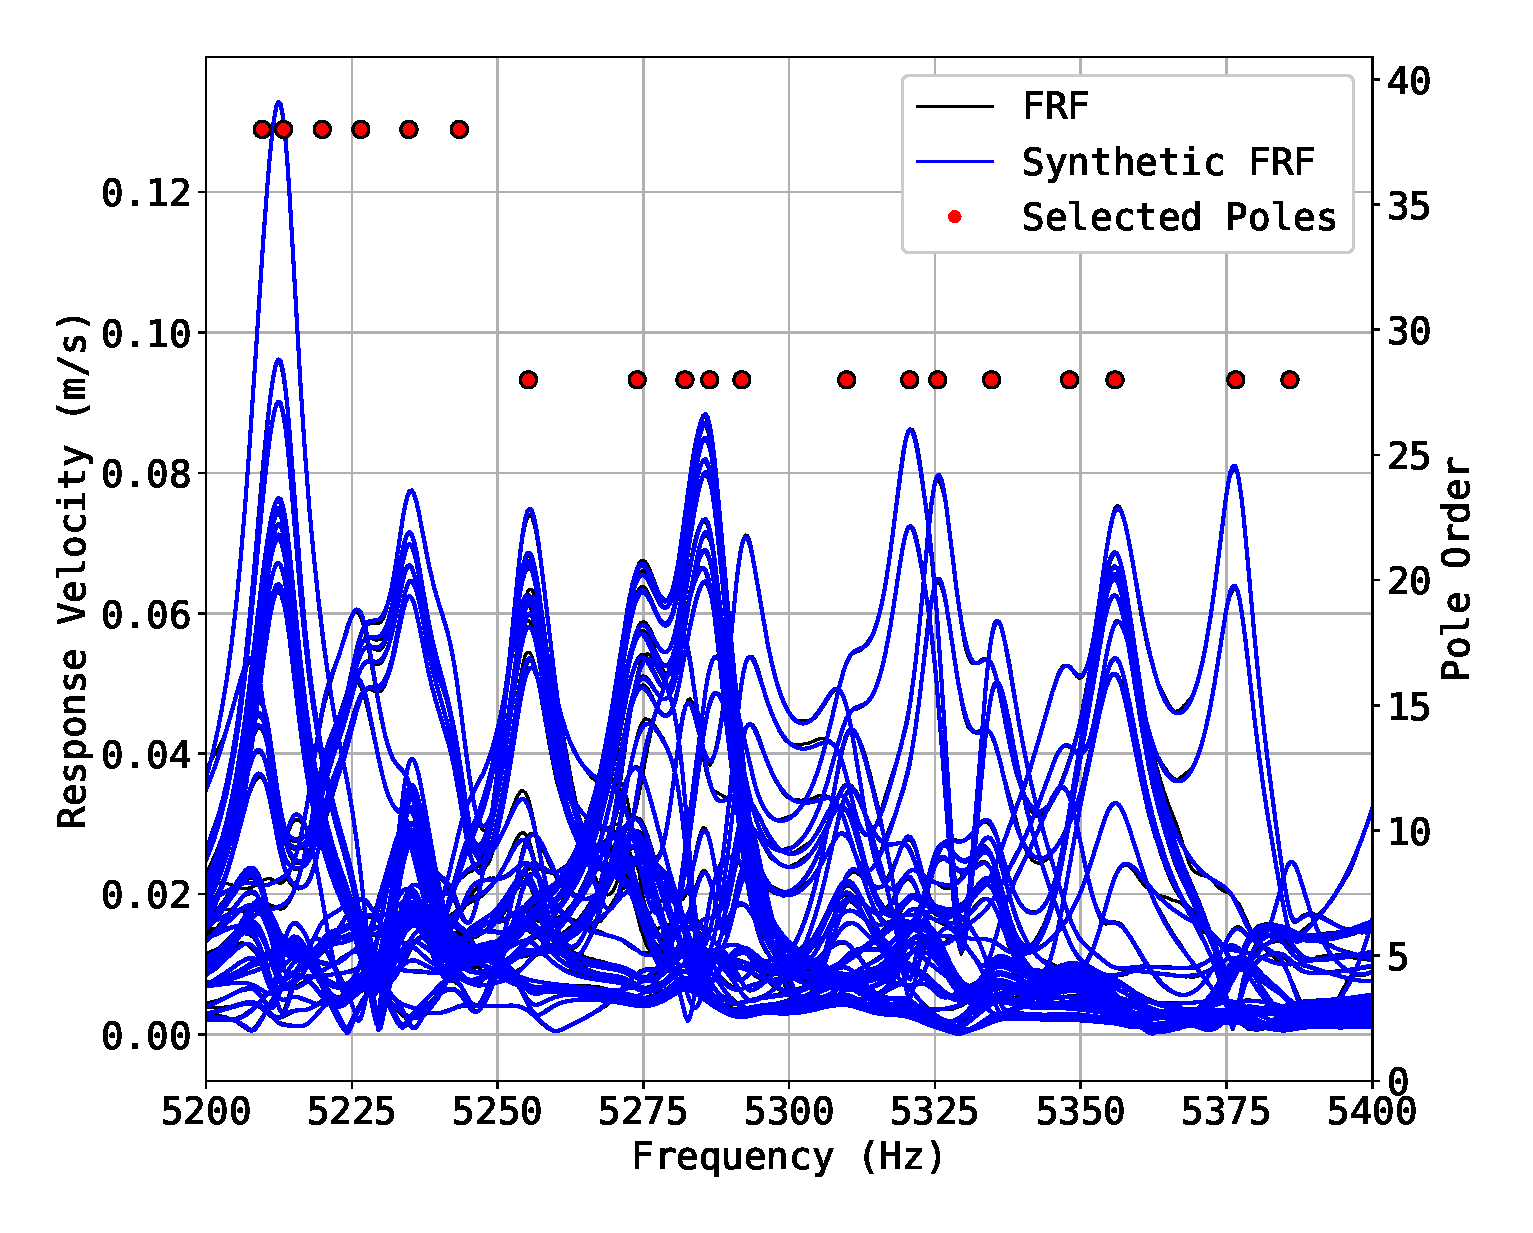
\includegraphics[width=\linewidth, trim=20 0 20 0, clip, alt = {pLSRA Applied to the Full Rotor}]{figures/full-rotor/Figure20.eps}
    \caption{Full rotor experimental and synthetic (pLSRA) FRF}
    \label{fig:twe-frf-selected-poles}
\end{figure}

A set of 40 modes was extracted from the experimental full rotor EO 5 and EO 7 TWE results using the same pLSRA algorithm used in the isolated blade experiment. As in the full GMM analysis, the modes from the two mode families of interest were concentrated within a narrow frequency range ($5042.3$--$5496.7$~Hz), with an average of $11.6$~Hz between modes, making accurate mode shape extraction challenging. However, collecting 3700 individual frequency responses over the entire rotor vastly improves the accuracy of pLSRA, and as Figure \ref{fig:twe-frf-selected-poles} shows, there is virtually no difference between the synthesized FRF and the experimental FRF with a FRAC of $0.9998$. This demonstrates pLSRA's effectiveness in extracting mode shapes despite the tightly spaced modes and modal energy confinement observed in this mistuned system.

\begin{figure}[h]
    \centering
    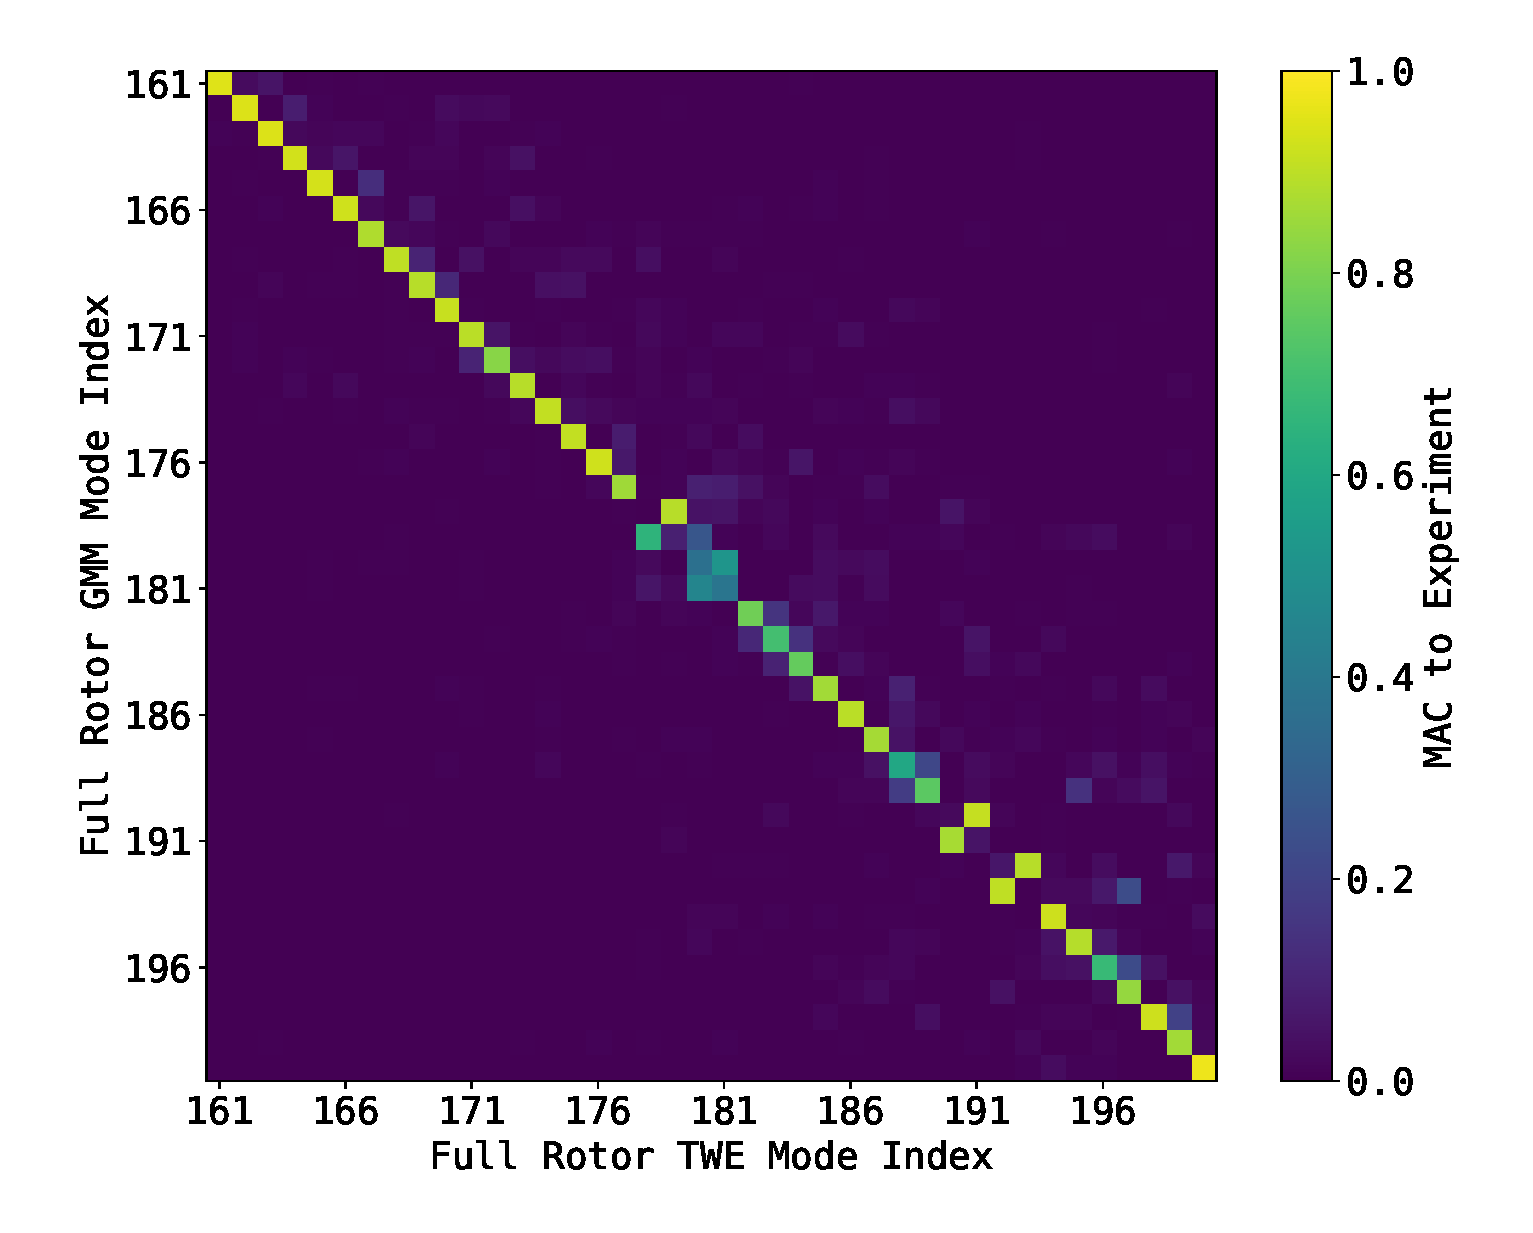
\includegraphics[width=\linewidth, trim=20 0 20 0, clip, alt = {TWE - Full Rotor Mode 176}]{figures/full-rotor/Figure21.eps}
    \caption{MACs of GMM to TWE -- Modes 161--201}
    \label{fig:gmm-exp-full-macs}
\end{figure}

Figure \ref{fig:gmm-exp-full-macs} shows the MAC scores between the predicted full rotor GMM and the observed TWE modes 161--201, showing the agreement in individual blade mode shape variation as well as mistuning amplification for the PBS Rotor 5. The MACs range from $0.4563$ to $0.9728$ with a high mean MAC of $0.8462$ along the diagonal despite the sensitivity of both modal energy confinement and mode swapping. Outliers include experimental modes 180 and 181, which have a MAC between them of $0.825$, indicating that these are duplicates rather than distinct modes. Additionally, there are three pairs of modes in the GMM whose order has been swapped relative to the experiment, all with 0.5--9.45~Hz between them. This helps to indicate how sensitive these modes are to even slight geometric variations within the GMM. Regardless, Figure \ref{fig:gmm-exp-full-macs} shows that the GMM can robustly predict the mistuned response of the PBS Rotor 5, despite the observed mode swapping between these two mode families.

\begin{figure}[b]
    \centering
    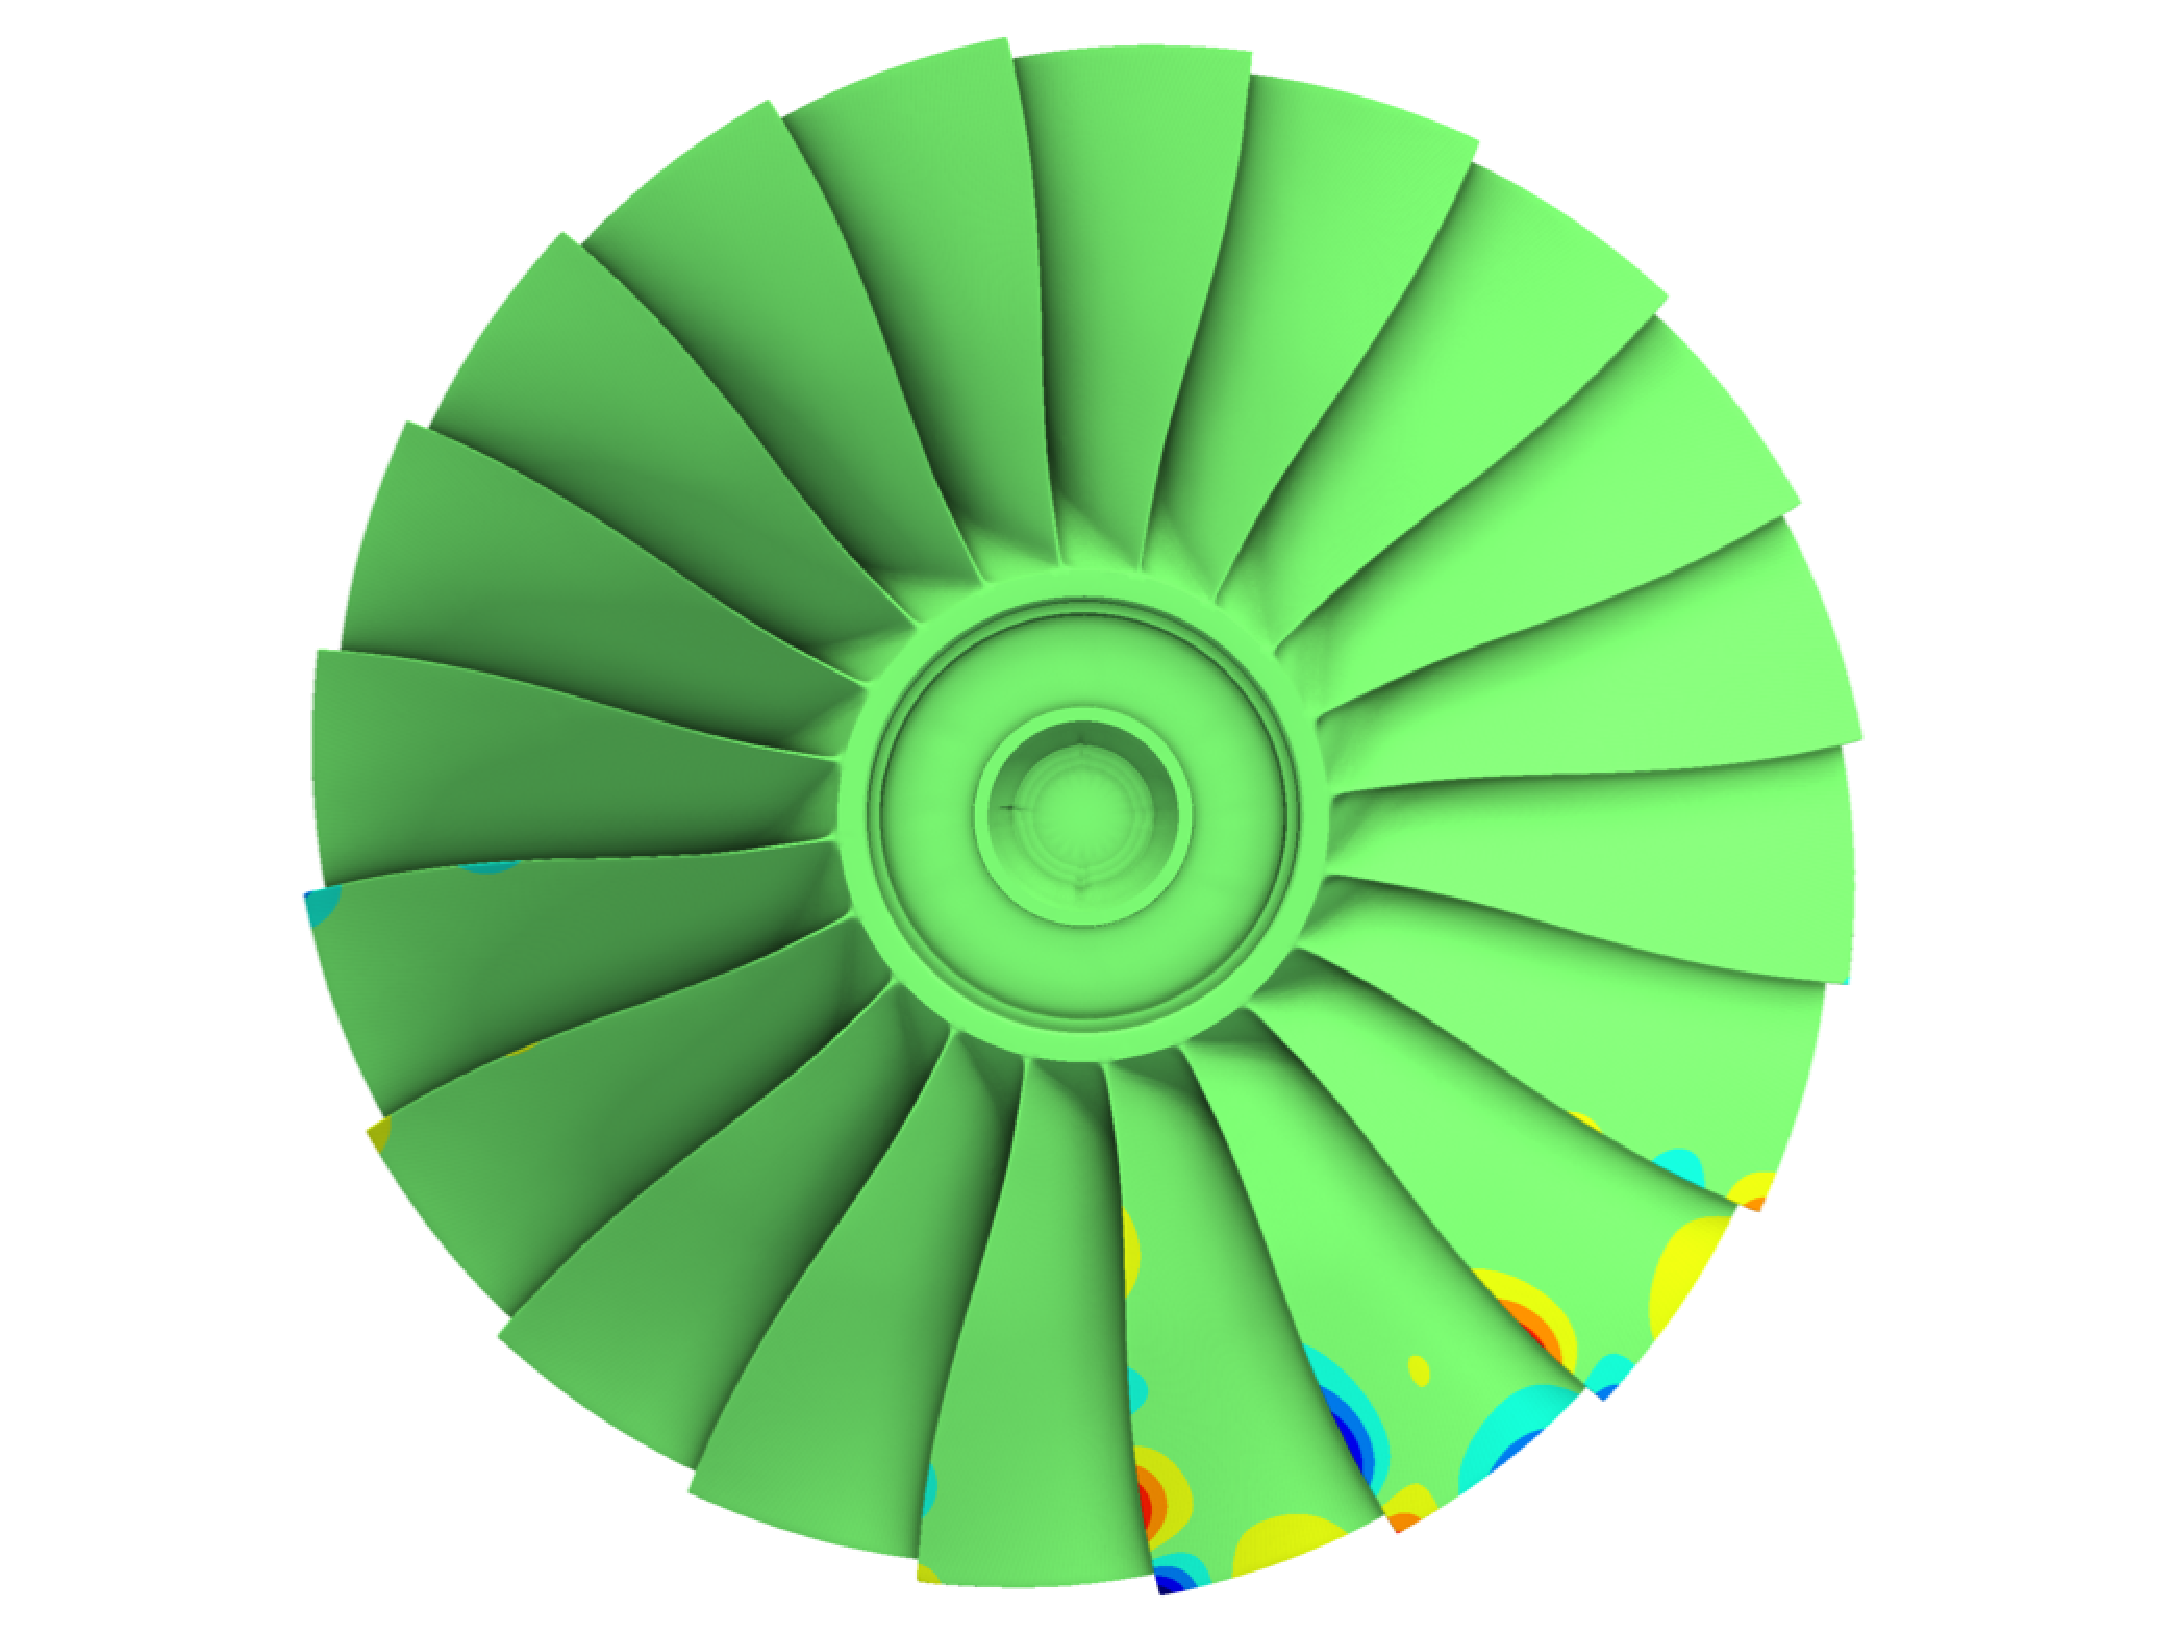
\includegraphics[width=0.5\linewidth, trim=140 0 120 0, clip]{figures/full-rotor/Figure22a.eps}%
    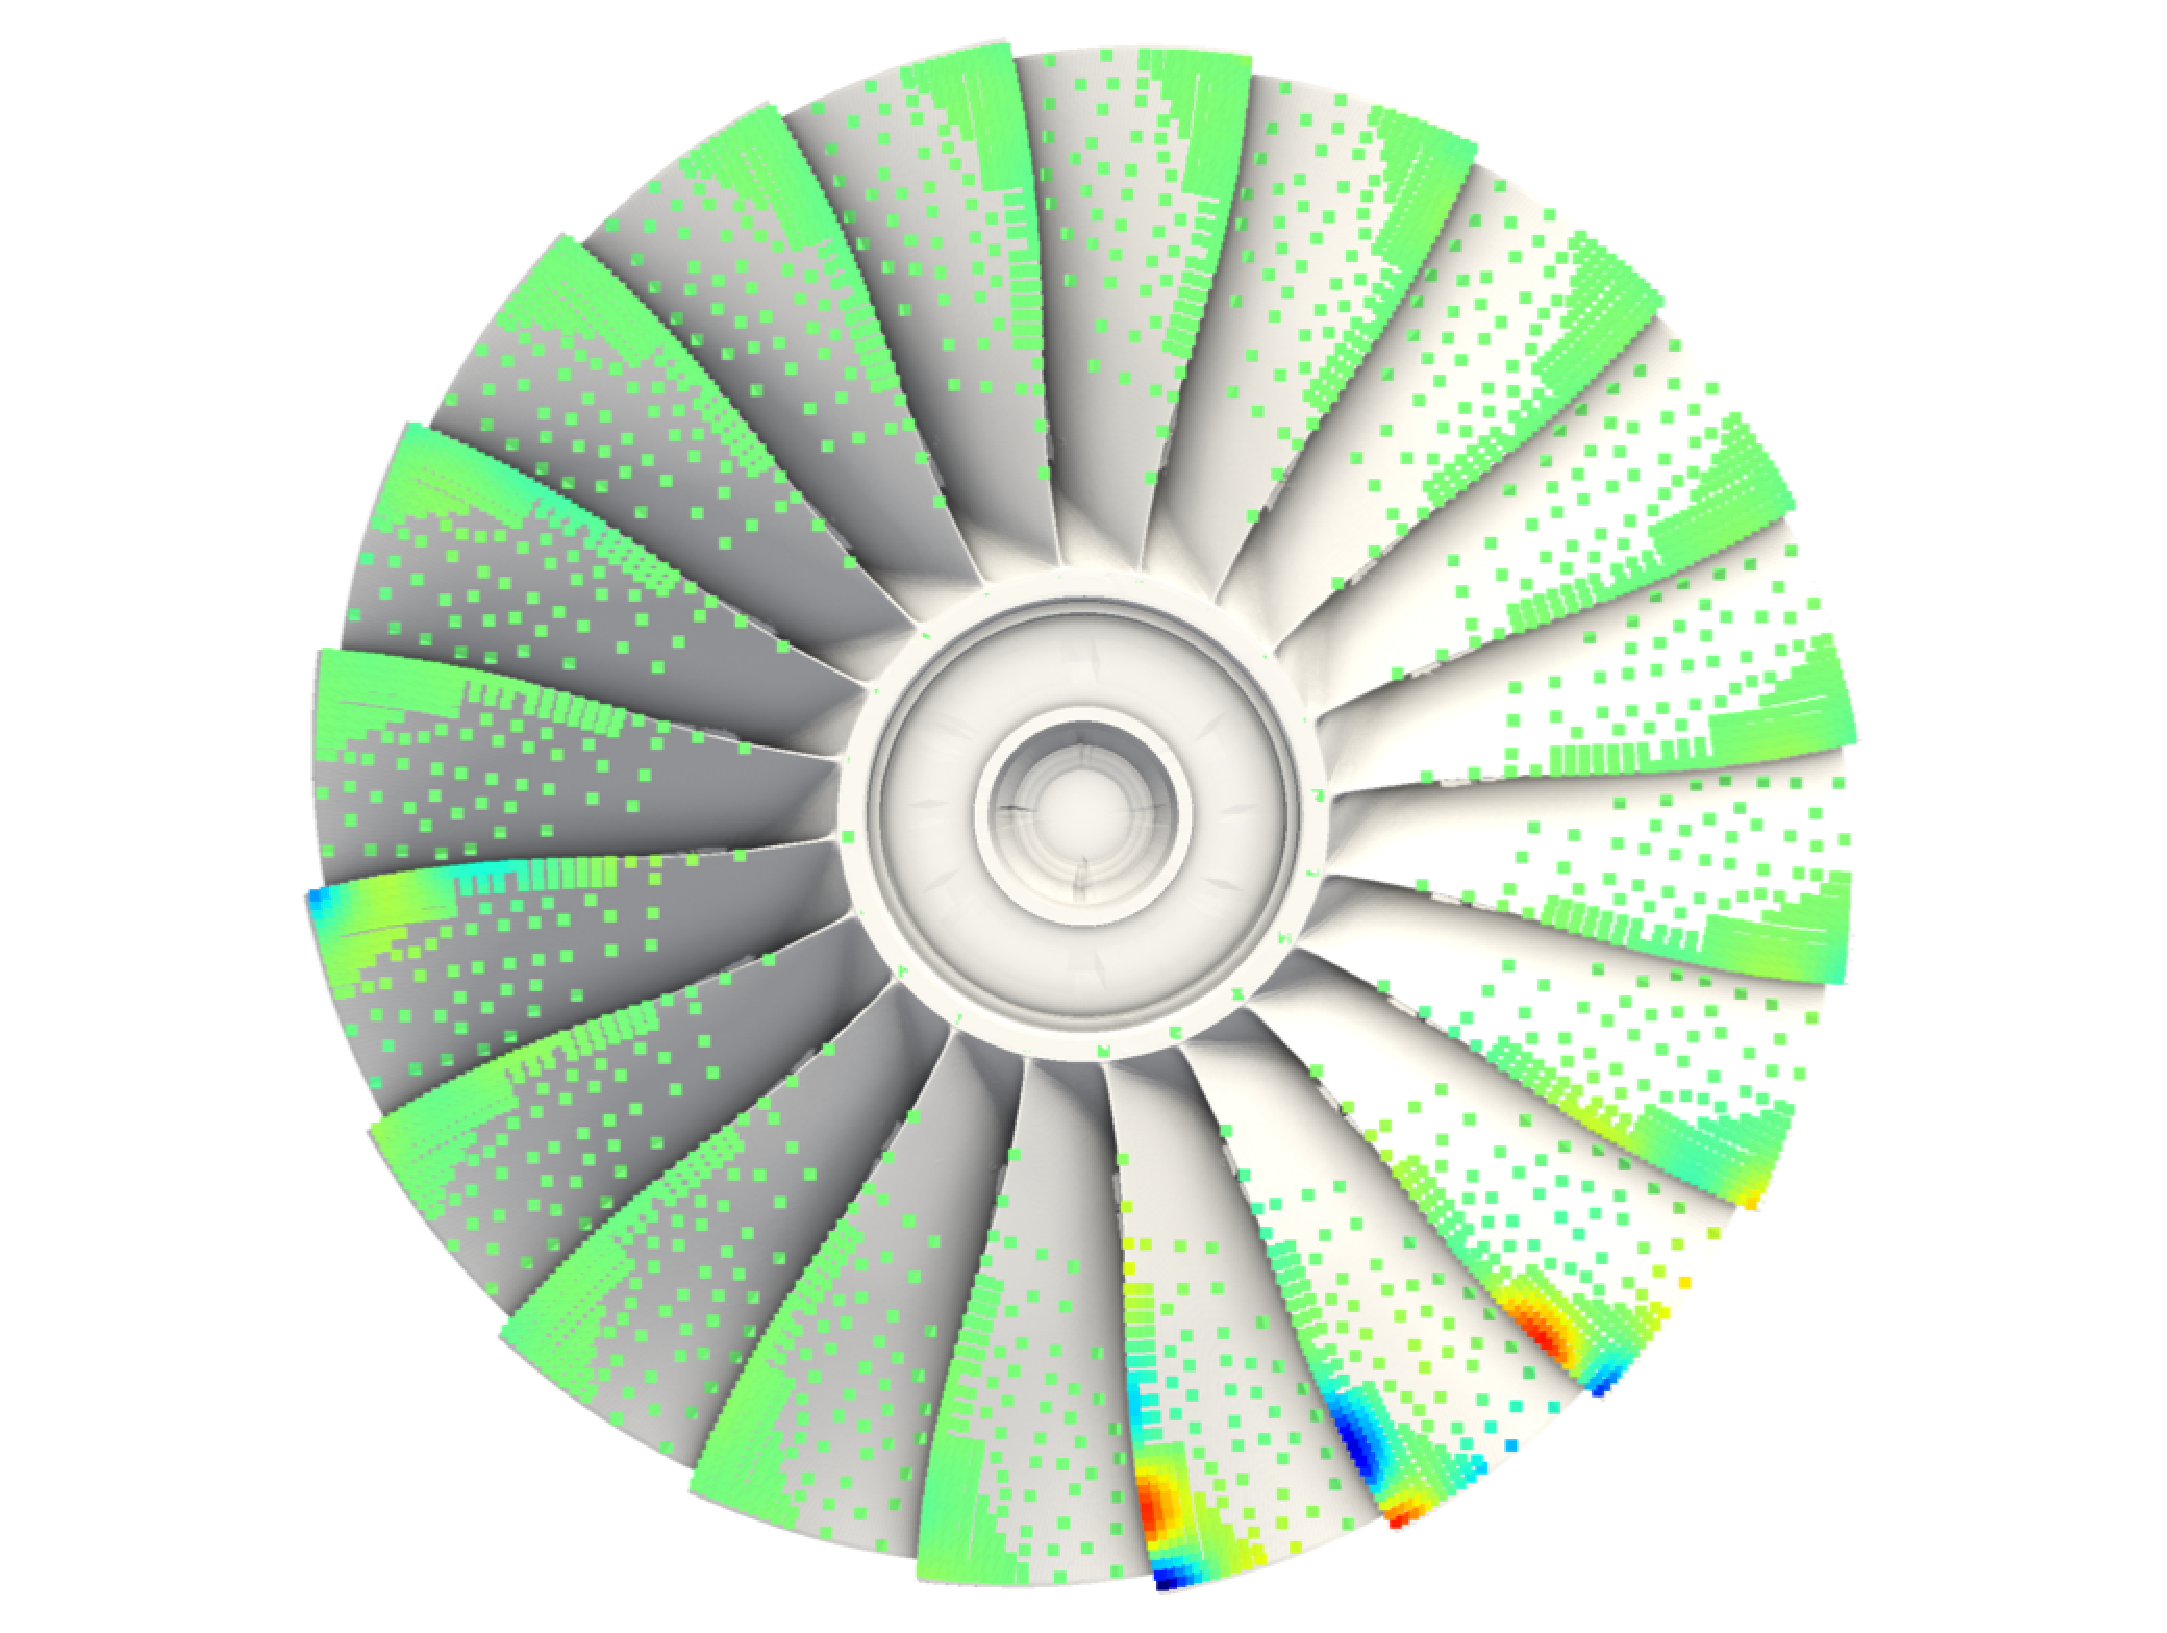
\includegraphics[width=0.5\linewidth, trim=120 0 140 0, clip]{figures/full-rotor/Figure22b.eps}
    \caption{Full rotor mode 192 -- GMM prediction (left) vs. mode from TWE (right)}
    \label{fig:full-rotor-mode-192-comparison}
\end{figure}

Figures \ref{fig:full-rotor-mode-176-comparison} and \ref{fig:full-rotor-mode-192-comparison} show modes 176 and 192, with MACs of $0.9275$ and $0.9042$ between the predicted (GMM) and experimentally observed (TWE) modes. Both the relative blade amplitude and individual blade mode shapes closely match the predicted full rotor GMM mode shapes. While not all modes showed this strong of an agreement, outside of the duplicate experimental modes, both the amplitude and individual blade mode shapes from the GMM strongly agree with the experiment despite the highly sensitive mode swap families. These results indicate that the predicted mistuning amplification and mode localization effects are reliable enough to predict mode swapping, and in the case of this mode pair, predict even full mistuned mode shapes. While the authors believe that the stochastic nature of mistuning prohibits reliable and precise prediction of mistuning amplification at low amplification factors ($< 2.5\times$), the modal analysis from the GMM and subsequent experimental validation demonstrate that GMMs can be used to robustly predict when and how mode swapping should occur.

\section{Conclusion}
The present work contributes new processes and the validation of part-specific modeling of mistuned rotors with an emphasis on blade mode shape variations. An accurate part-specific FEM is created through mesh morphing to optical scan data generated from an iterative process, which enables measurement error reduction. The results of this model are compared to experimental data generated by a traveling wave excitation system and LDV measurements of 185 measurement points per airfoil of the 20-bladed test rotor. The dense pattern of blade vibration measurements is used to validate a part-specific model's ability to predict inter-blade mode shape variations with a focus on extreme variation of a closely spaced mode pair. Experimental data is collected for both the mistuned rotor and isolated blades by using mass detuning and blade damping. Mistuned system identification based on FMM ID is used to extract blade mistuning parameters, and pLSRA is used to identify both blade test frequencies and mode shapes for isolated and full rotor experimental TWE results.

The results show that optical measurement data can be used to create GMMs that have high correlation with both isolated airfoil and full mistuned system response. The pLSRA approach was further found to perform well for isolated blade and full rotor testing configurations. The complex dynamics of closely coupled mode families were experimentally characterized, and the GMM was effective even in this nonlinear region. This work gives further confidence in the use of GMMs as an effective method to design and manage modern IBRs.

\section*{Acknowledgments}

PyVista \cite{Sullivan2019} was used for 3D visualization, figure generation, and 3D model analysis in this research.

\bibliographystyle{asmeconf}
{\footnotesize
    \bibliography{references}
}

\raggedbottom

\pagebreak

\appendix

\section[Mode Comparison Table]{Mode Comparison Table of Identified vs. GMM Modes}\label{appendix:mode_comparison}

Table~\ref{tab:appendix-mode-comparison} (at the end of the paper) shows the correlation between the experimentally identified sector mistuning deviations ($\Delta_{\omega}$) and the GMM-predicted values. The high correlation and matching frequency ranges show that the GMM accurately predicts the full mistuned system.

\section[Standard Deviation of FMM ID Mode Families]{Standard Deviation of FMM ID Mode Families}\label{appendix:fmm_std_dw}

Table~\ref{tab:appendix-fmm-std} (at the end of the paper) shows the standard deviation of the FMM ID sector mistuning deviations ($\Delta_{\omega}$) for the mode families of interest. The mean standard deviation of the sector mistuning deviations from FMM ID is $0.016853$.

\section[Mode Figures]{Mode Shape Variation -- Mode 14}\label{appendix:mode_shape_variation}

\renewcommand{\thefigure}{B\arabic{figure}}%
\renewcommand{\theHfigure}{\thefigure}%
\setcounter{figure}{0}%
\begin{figure}
    \centering
    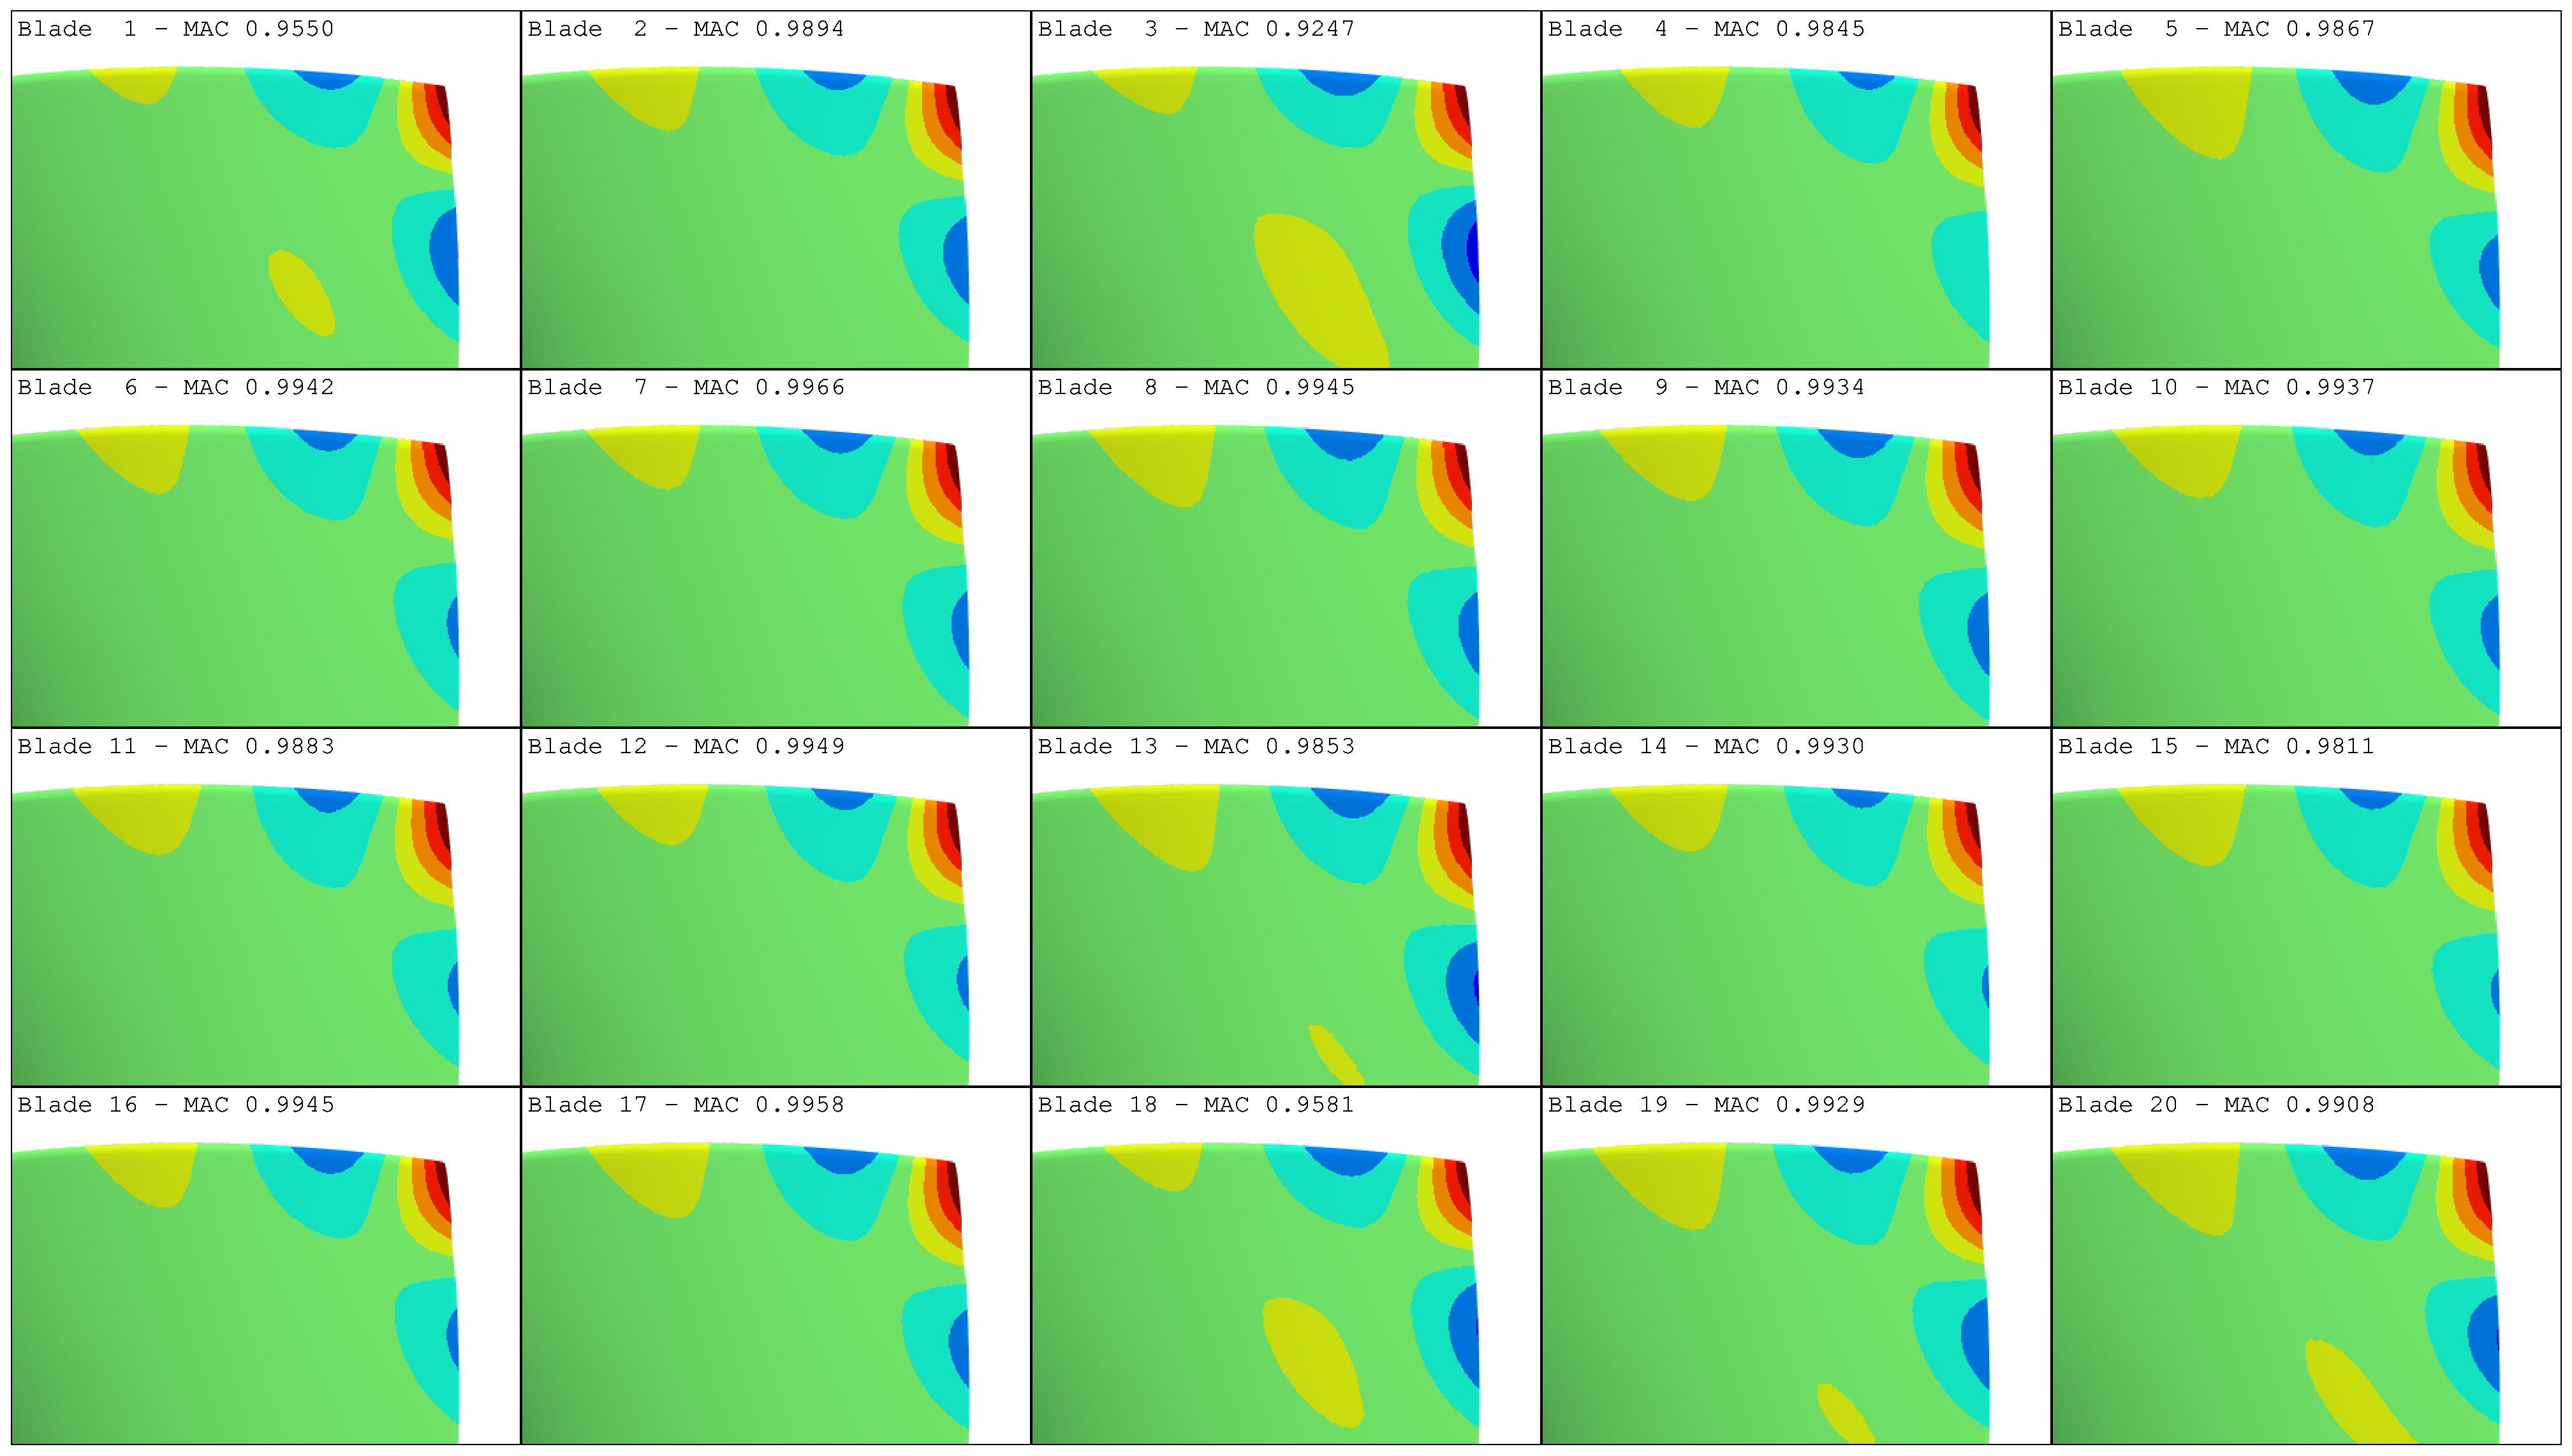
\includegraphics[width=\linewidth, alt = {Mode shape of all blades of mode 14 for the GMM}]{figures/mode-14-gmm/FigureB1.eps}
    \caption{Blade mode shape from GMM -- mode 14}
    \label{fig:mode-14-all-ms-gmm}
\end{figure}

Figure \ref{fig:mode-14-all-ms-gmm} shows the mode-to-mode shape variation for Mode 14 from the GMM. MAC values within the figure are between the tuned mode shape and the individual blade mode shapes as shown in each square. It should be noted that this mode, according to Figure \ref{fig:mac-scatter} and Table \ref{tab:iso-exp-table}, still shows significant mode shape variation despite not exhibiting mode swapping with adjacent modes. Figure \ref{fig:mode-14-le-disp} shows the normalized mode shape across the leading edge of mode 14.

\begin{figure}
    \centering
    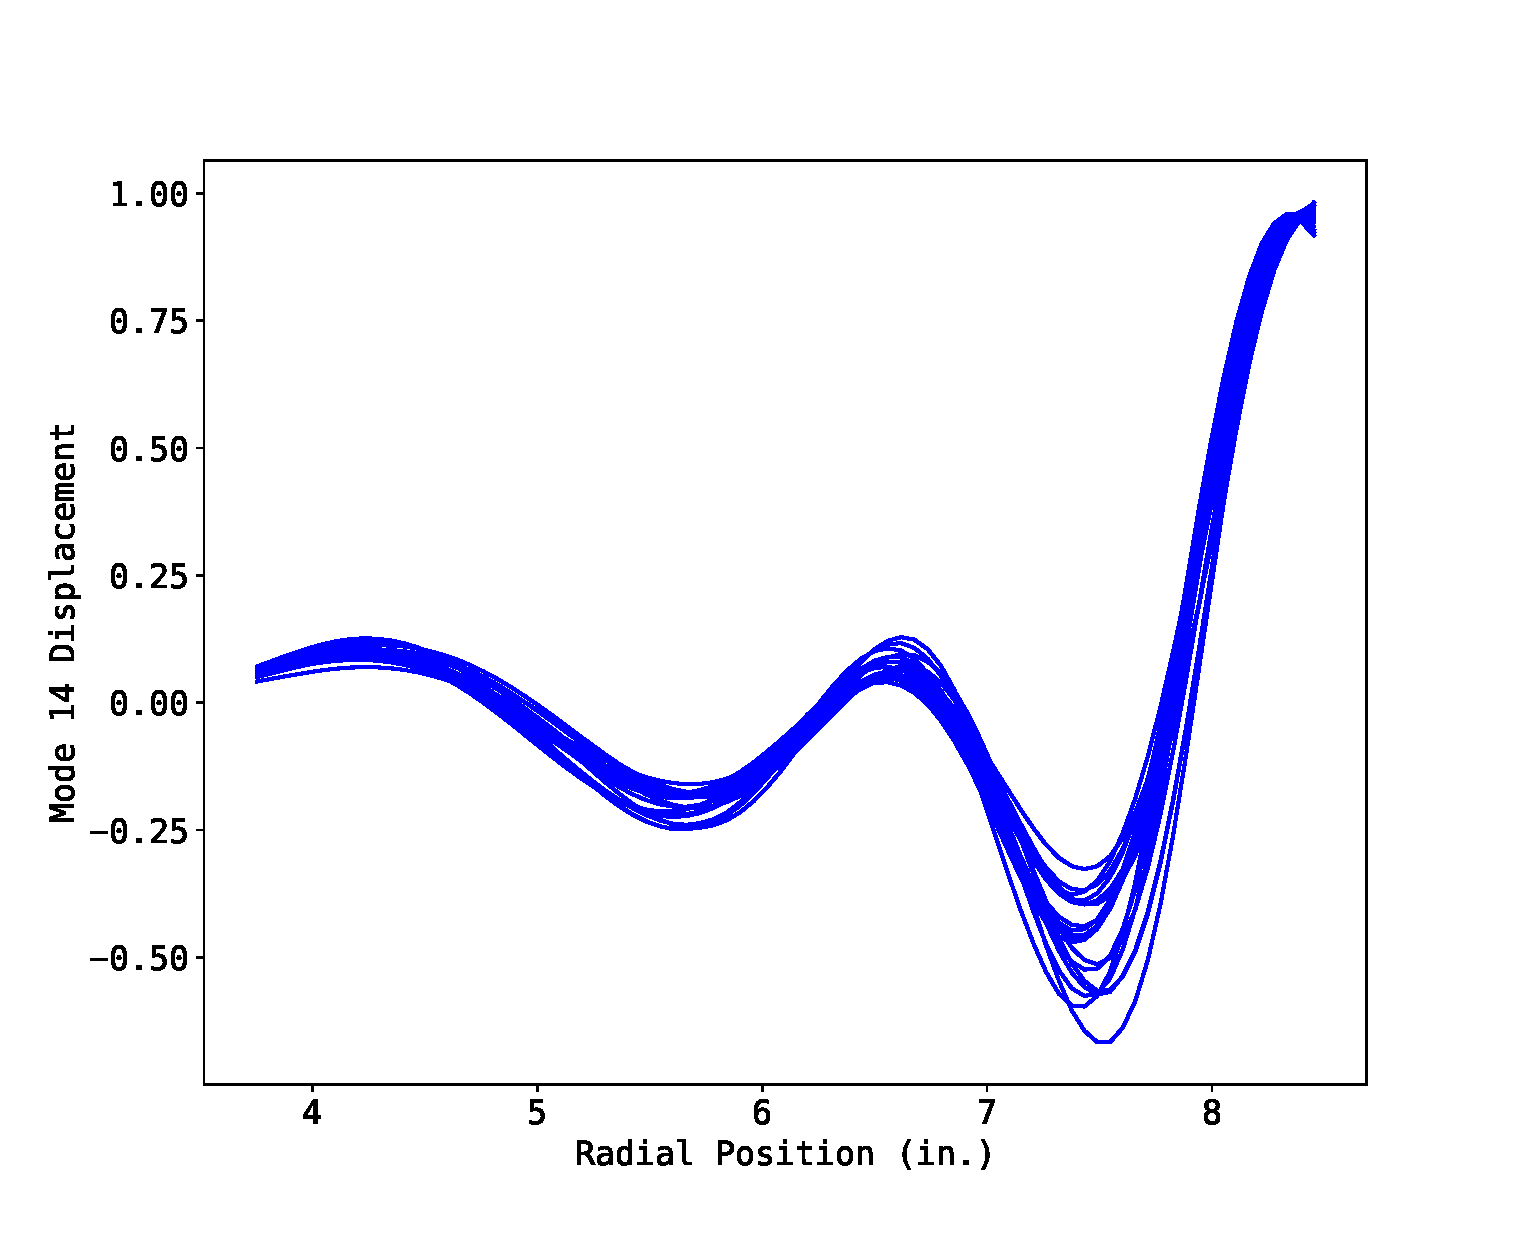
\includegraphics[width=\linewidth, alt = {Mode shape of all blades of mode 14 for the GMM}]{figures/mode-14-gmm/FigureB2.eps}
    \caption{Leading edge mode shape from GMM -- mode 14}
    \label{fig:mode-14-le-disp}
\end{figure}

\clearpage
\onecolumn

\renewcommand{\listfigurename}{Figure Captions}
\listoffigures

\clearpage
\listoftables

\clearpage
\begin{center}
    \captionof{table}{Isolated sector correlation between experimental, GMM, and FMM results (second and third columns) and intrablade MAC scores for the experimentally identified isolated blade mode shapes (fourth and fifth columns)}
    \label{tab:iso-exp-table}
    \begin{tabular}{rrrrr}
    \hline
    $\omega_i$ & $r_{\Delta_{\omega}{\text{ISO},\text{GMM}}}$ & $r_{\Delta_{\omega}{\text{ISO},\text{FMM}}}$ & $\overline{\mathrm{MAC}}_{i=j}$ & $\overline{\mathrm{MAC}}_{i<j}$ \\
    \hline
    1          & 0.9654                                       & 0.9526                                       & 0.9971                          & 0.9968                          \\
    2          & 0.9914                                       & 0.9923                                       & 0.9969                          & 0.9927                          \\
    3          & 0.9682                                       & 0.9920                                       & 0.9980                          & 0.9961                          \\
    4          & 0.9929                                       & 0.9919                                       & 0.9834                          & 0.9690                          \\
    5          & 0.9619                                       & 0.9527                                       & 0.9365                          & 0.9061                          \\
    8          & 0.9944                                       & 0.9990                                       & 0.9644                          & 0.9629                          \\
    9          & 0.9816                                       & 0.9670                                       & 0.8948                          & 0.7071                          \\
    10         & 0.9915                                       & 0.9562                                       & 0.9026                          & 0.5737                          \\
    12         & 0.9986                                       & 0.9985                                       & 0.9776                          & 0.9515                          \\
    13         & 0.9968                                       & 0.9937                                       & 0.9721                          & 0.9367                          \\
    14         & 0.9985                                       & 0.9949                                       & 0.9702                          & 0.9230                          \\
    15         & 0.9962                                       & 0.9952                                       & 0.9346                          & 0.8977                          \\
    16         & 0.9986                                       & 0.9900                                       & 0.9788                          & 0.9373                          \\
    \hline
\end{tabular}

\end{center}

\clearpage
\renewcommand{\thetable}{A\arabic{table}}%
\renewcommand{\theHtable}{\thetable}%
\setcounter{table}{0}%
\begin{center}
    \captionof{table}{Mode comparison of experimentally identified versus GMM-predicted modes and the correlation of their sector mistuning deviations}
    \label{tab:appendix-mode-comparison}
    \begin{tabular}{rllr}
\hline
   $\omega_i$ & Experiment          & GMM                 &   $r_{\Delta_{\omega}{\text{FMM},\text{GMM}}}$ \\
\hline
             1 & 566 -       666 Hz  & 569 -       729 Hz  &       0.9794 \\
             2 & 1553 -      1756 Hz & 1567 -      1687 Hz &       0.9881 \\
             3 & 1821 -      1921 Hz & 1808 -      1873 Hz &       0.9731 \\
             4 & 2617 -      2953 Hz & 2734 -      2931 Hz &       0.9924 \\
             5 & 3012 -      3241 Hz & 2920 -      3231 Hz &       0.9859 \\
             6 & 3575 -      3812 Hz & 3513 -      3833 Hz &       0.9583 \\
             7 & 3989 -      4278 Hz & 4027 -      4283 Hz &       0.9329 \\
             8 & 4424 -      4815 Hz & 4412 -      4776 Hz &       0.9942 \\
             9 & 4944 -      5624 Hz & 4982 -      5412 Hz &       0.9884 \\
            10 & 5074 -      5471 Hz & 5086 -      5400 Hz &       0.9428 \\
            11 & 5809 -      6503 Hz & 5912 -      6468 Hz &       0.9922 \\
            12 & 6597 -      7193 Hz & 6600 -      7114 Hz &       0.9622 \\
            13 & 7237 -      7842 Hz & 7016 -      7671 Hz &       0.8899 \\
            14 & 7301 -      8215 Hz & 7355 -      8075 Hz &       0.9962 \\
            15 & 7950 -      8800 Hz & 8153 -      8653 Hz &       0.9968 \\
            16 & 8640 -      9255 Hz & 8530 -      9173 Hz &       0.9926 \\
            17 & 9132 -      9851 Hz & 8977 -      9601 Hz &       0.9188 \\
\hline
\end{tabular}

\end{center}

\clearpage
\begin{center}
    \captionof{table}{Standard deviation of the FMM ID sector mistuning deviations by mode family}
    \label{tab:appendix-fmm-std}
    \begin{tabular}{rr}
    \hline
    $\omega_i$ & $\sigma_{\Delta_{\omega}, \text{FMM}}$ \\
    \hline
    1          & 0.0090                                 \\
    2          & 0.0106                                 \\
    3          & 0.0053                                 \\
    4          & 0.0157                                 \\
    5          & 0.0121                                 \\
    8          & 0.0207                                 \\
    9          & 0.0198                                 \\
    10         & 0.0170                                 \\
    12         & 0.0214                                 \\
    13         & 0.0238                                 \\
    14         & 0.0260                                 \\
    15         & 0.0161                                 \\
    16         & 0.0216                                 \\
    \hline
\end{tabular}

\end{center}

\end{document}
